\chapter{Qu'est ce qu'un angle\,?}
\label{chap_angle}
% je remets ça là pour pas avoir les mêmes numéros d'axiomes dans différentes parties.
\newcounter{serieaxiom}
\setcounter{serieaxiom}{1}
\newcounter{axinum}
\setcounter{axinum}{1}
\renewcommand{\theaxi}{\Alph{serieaxiom}.\arabic{axi}}


%\initial{L}{'angle} est comme tout ce qui semble évident, plutôt laborieux à définir. Dans son acception ancienne l'angle représente une portion de plan entre deux demi-droite, le secteur d'angle, alors qu'aujourd'hui elle se confond souvent avec la mesure de l'angle. Ces représentations ne sont pas fondamentalement en désaccord une fois déployé l'ensemble les distinctions et relations qui les lient. 

%\remarquehistoireimage{On sait peu de chose de la vie d'Euclide sinon qu'il aurai vécu autour du \Romanbar{3}\iemes siècle avant notre ére. Son ouvrage : \href{http://promenadesmaths.free.fr/telecharger/euclide_elements_1804.pdf}{Éléments} contient une tentative quasiment aboutit de construction d'une géométrie axiomatique. Il contient de nombreux théorème et leurs démonstrations. Il connue de nombreuses éditions et les copies successives contiennent des ajouts ou modifications de ceux qui les produire de sorte que le texte qui nous est parvenue n'est pas tout a fait le texte produit par Euclide. On peut néanmoins supposer que ces modifications respectent l'esprit d'Euclide. Son contenue reste au centre de l'enseignement de la géométrie du secondaire.}{image/EuclideGravure.jpg}

%Une tentative de construction des ces axiomes fut pour la première fois établis par Euclide dans ses \href{http://promenadesmaths.free.fr/telecharger/euclide_elements_1804.pdf}{Éléments}. En 1899, les << \'Eléments >> d'Euclide ne satisfont plus les mathématiciens. Non pour ses éventuelles limitations, mais parce que justement le système d'axiome proposé par Euclide est lacunaire. Plusieurs fois, dans la lecture des \emph{éléments}, on remarque que certains résultats, implicitement considérés comme vrai, sont utilisés sans avoir fait l'objet de démonstrations. Et pour cause, avec les axiomes présents, ils sont indémontrable. Le but de la relecture par Hilbert est de proposer un système d'Axiome suffisant, respectant l'esprit de la construction Euclidienne et permettant d'aboutir à la même géométrie. Il publiera les résultats de ses travaux dans un livre : <<\href{https://www.pedagogie.ac-aix-marseille.fr/upload/docs/application/pdf/2019-11/principes_fondamentaux_geometrie_-_david_hilbert.pdf}{Les principes fondamentaux de la géométrie}>> qui sera traduit et publié en français en 1900. C'est dans l'esprit axiomatique de Hilbert que nous présenterons dans cette sections 

%\remarquemargehistoireimage{David Hilbert (1862-1942) est un mathématicien Allemand ayant travaillé principalement a l'université de Göttingen. Il est connue pour sa ré-axiomatisation de la géométrie d'Euclide mais aussi ses traveaux autour des espace di de Hilbert, \cad des espaces vectoriels (réels où complexe) sur lequel est définie un produit scalaire et complet pour la distance issue du produit scalaire. Il vivra très difficilement l'exclusion de ses collègue juifs loirs de la période nazi et lorsque la ministre nazi lui demandera : \og Comment se trouvent les mathématiques à Göttingen maintenant qu'elle est libre de l'influence juive ? \fg Hilbert répliquera : \og Des mathématiques à Göttingen ? Il n'y en a plus guère \fg. Sur sa tombe est gravé \og Wir müssen wissen, wir werden wissen \fg : soit \og Nous devons savoir, nous saurons\fg. }{image/Hilbert.jpg}{15cm}

    %\section{Notion première}\label{subsec-notionpremiere}
    
    %\section{Pourquoi reprendre aux niveaux des axiomes?}
\begin{quote}
    Le bien connu en général, pour la raison qu'il est bien connu, n'est pas connu. C'est la façon la plus commune de se tromper et de tromper les autres, à propos du connaître, que de présupposer quelque chose comme bien connu.

    Georg Wilhelm Friedrich Hegel, \emph{Phénoménologie de l’esprit.}
\end{quote}
%\epigraph{Le bien connu en général, pour la raison qu'il est bien connu, n'est pas connu. C'est la façon la plus commune de se tromper et de tromper les autres, à propos du connaître, que de présupposer quelque chose comme bien connu.}{Georg Wilhelm Friedrich Hegel, Phénoménologie de l’esprit}

%\addlb{Commentaire général\,: tu pars beaucoup trop dans tous les sens en évoquant plein de notions avancées qui ne sont pas abordées dans le texte (ex : séries entières). Donc la majorité de ton intro est hors sujet et illisible. Seul le dernier paragraphe, dans lequel tu annonces l'objectif du chapitre, est vraiment pertinent. Ton introduction historique suppose déjà une connaissance assez solide des mathématiques, et est donc illisible pour notre public. Il faut quasiment tout récrire.}

\initial{S}{i} la construction axiomatique de la géométrie a été pour la première fois portée par Euclide, la liste d'axiomes qu'il propose est incomplète. Certains résultats, implicitement considérés comme vrai, sont utilisés sans avoir fait l'objet de démonstrations. Et pour cause, avec les axiomes présents, ils sont indémontrable. On se placera par conséquent d'avantage dans la formulation faite par Hilbert \cite{HilbertLesPF}. 
% \guil{\href{https://www.pedagogie.ac-aix-marseille.fr/upload/docs/application/pdf/2019-11/principes_fondamentaux_geometrie_-_david_hilbert.pdf}{Les principes fondamentaux de la géométrie}}. 

%qu'on peut qualifier d'axiomatique synthétique.

Les axiomatiques d'Euclide et de Hilbert ont ceci en commun qu'elles s'appuient toutes deux sur les notions premières de points, de droite, de plan, d'appartenance, d'union et d'intersection. On parle d'axiomatique synthétique. Cette notion d'axiomatique synthétique où de géométrie synthétique est apparue au cours du \Rom{19} $^\e$ siècle par opposition a la géométrie analytique, celle qui repose sur les nombres, le calculs. Dans la pratique vraiment concrète des mathématiques cette opposition est une précieuse ridicule typique des querelles de mathématiciens. Jean Dieudonné qualifiera cette opposition de \guil{grotesques querelles des géomètres "synthétiques" et des géomètres "analytiques", aussi incompréhensibles pour nous que les discussions byzantines sur le sexe des anges, ont rempli des volumes au XIX$^\e$ siècle}. Euclide \cite{euclidelements} ne s'embarrasse pas d'une telle opposition\,: dès les axiomes de ses \guil{\href{http://promenadesmaths.free.fr/telecharger/euclide_elements_1804.pdf}{éléments}}, sa construction de la géométrie mélange axiomes synthétiques et axiomes analytiques. Néanmoins à mesure que se développe l'exposé de résultats majoritairement synthétiques (par exemple nombre de points dans l'intersection de deux droites), on passe à une majorité de résultats qu'on pourrait qualifier d'analytiques (Théorème de l'angle extérieur, Thalès ou encore Pythagore). Bref, à mesure que se déploie la géométrie chez Euclide ou même à travers l'histoire, les mathématiciens partent d'objets géométriques (synthétiques) pour en déduire des propriétés analytiques qui leurs sont attachées (Al-Kashii, volume du cône, surface sous la parabole, volume d'une sphère). Les résultats analytiques furent si nombreux que dès Pythagore, nombreux sont ceux qui pensèrent que \guil{tout est nombre}. Ce n'est cependant qu'après assimilation de la notion de repère Cartésien (présenté par Descartes dans \guil{\href{http://www.ffn.ub.es/luisnavarro/nuevo_maletin/Descartes\%20(1637)_Geometrie.pdf}{La géométrie, livre premier}} \cite{descartesgeometrie} \footnote{Disponible ici \url{http://www.ffn.ub.es/luisnavarro/nuevo_maletin/Descartes\%20(1637)_Geometrie.pdf}}) qu'on pouvait, sans nul doute, penser pouvoir reconstruire la géométrie uniquement à partir des nombres. Or la constructions axiomatique des nombres en particulier, les nombres réels, devra attendre 1869 (Meray, Cantor) et Dedekind (1872). Cette difficulté dans l'axiomatisation des nombres réels est une des cause du caractère parfois hasardeux de certaine démonstration d'Euclide. Sans nombres réels la notion de distance est susceptible d'être conçue de façon bancale. 



La reconstruction de la géométrie par les nombres et à partir des nombres uniquement (géométrie affine ou analytique) à travers la notion d'espace vectoriel, puis d'espace vectoriel euclidien (par Hilbert également) va permettre un vaste déploiement de nouveaux résultats. Elle va permettre de formaliser toute une gamme de géométrie non-euclidienne (variété topologique, différentiable, Riemannienne). Ces géométries d'abords découvertes à travers la tentative infructueuse de démontrer le cinquième axiome d'Euclide, l'axiome des parallèles, devait, si l'ont voulait les construire avec une axiomatique synthétique, utiliser chacune sa liste d'axiomes. Ce qui est long, et laborieux. Au \Rom{19}$^\e$ siècle, le souffle de la devise Pythagoricienne semblait irrésistible et c'est la raison de la réaction fondant le courant de géométrie synthétique. 
\FigureMarge{Solutions du problème d'Appolonius.}{1.2}{image/Appolonius.png}
L'approche synthétique était justifiée pour des problème comme le problème d'Appolonius (chercher les cercles tangents à trois cercles donnés dans le plan, voir figure ci contre) dont la résolution par une approche analytique est longue et ardue alors que sa résolution synthétique est courte et élégante. Dans tout les cas, avant cette formalisations affine des géomètries non-euclidienne, les mathématiciens travaillent dans certaines d'entre elle (Sphère, Lobatchevkii, disque de Poincarré) classées souvent en deux ensembles (Hyperbolique ou Elliptique) suivant la façon qu'elle ont de nier l'axiome des parallèles. Ces géométries suivent donc une axiomatique dans l'esprit d'Euclide, a mi chemin entre une approche synthétique et une approche analytique. L'exigence démonstrative a monté en gamme depuis Euclide et c'est dans dans cette approche que Hilbert va chercher a refonder une axiomatique engendrant la géomètrie d'Euclide. Cette exigence de rigueur va le pousser à adopter une axiomatique purement synthétique, remplaçant les notions de longueur ou de mesure d'angle par la notion de congruence (qu'il axiomatisera). Au bout d'un certains déploiement, et en y adjoignant l'axiomatique des nombres, ces notions de longueurs et de mesure d'angles sont reconstructibles ainsi que toute la géométrie d'Euclide. 





Le but du présent chapitre est de déployer entièrement la notion d'angle et de mesure d'angle. Dans son acception ancienne l'angle représente une portion de plan entre deux demi-droites, le secteur d'angle, alors qu'aujourd'hui elle se confond souvent avec la mesure de l'angle. Ces représentations ne sont pas fondamentalement en désaccord une fois déployé l'ensemble les distinctions et relations qui les lient. Mais alors pourquoi partir de l'axiomatique de Hilbert\,? Pourquoi réexploiter cet attirail dans un cours comme celui-ci\,? Pourquoi ne pas faire une approche affine (espace vectoriel euclidien)\,? Ou une approche semi-intuitive, semi-synthétique, semi-analytique à la Euclide\,?  À la première question de l'emploi de la géométrie fondée sur les espaces vectoriel, nous répondrons que cette approche est plus calculatoire, aspect des mathématiques que nous avons déjà vastement exploré dans les autres parties de ce cours. La principale raison est que cette approche nécessiterait une autre artillerie moins immédiatement géométrique pour être déployé. Une autre raison est que nous souhaitons, dans cette partie, familiariser le lecteur avec une mathématiques plus déductive, plus éloigné du nombre est du calcul et se concentrer nos effort sur la déduction et la démonstration. Enfin nous souhaitons faire apparaître la notion de cosinus et de sinus à partir de l'angle et donc de la figure, non à partir du calculs comme cela se ferait dans l'approche affine. À la seconde question de l'emploi de l'approche Euclidienne, certaines de ces démonstrations, a travers les résultats implicites non démontré, et \emph{non démontrable}, permettent d'appréhender mais pas de comprendre ce qu'est une preuve. L'approche de Hilbert, si son emploi dans toutes les partie du cours visant à obtenir des résultats et des formules utilisables par d'autre science est inutile, elle peut permettre, je le pense, d'acquérir l'esprit de la preuve en mathématique. Sur quelque chose qu'on pense bien connue : l'angle en géométrie. Qu'est ce qu'un angle\,? Dans l'esprit de la maxime de Hegel introduisant le chapitre 6\,: nous souhaitons montrer à quel point ce qui est conçu comme évident (içi l'angle) nécessite pour être conçu concrètement (\cad dans toutes ses déterminations) un travaille long et laborieux. L'axiomatique de Hilbert nous permettra d'atteindre ce but. 

%\citeauthor{descartesgeometrie}

%\addlb{[Tu ne reponds pas `a cette question ! D’autant plus que c’est l’approche que j’ai l’habitude d’utiliser lorsque je donne cours `a des debutants en maths.]LB }

%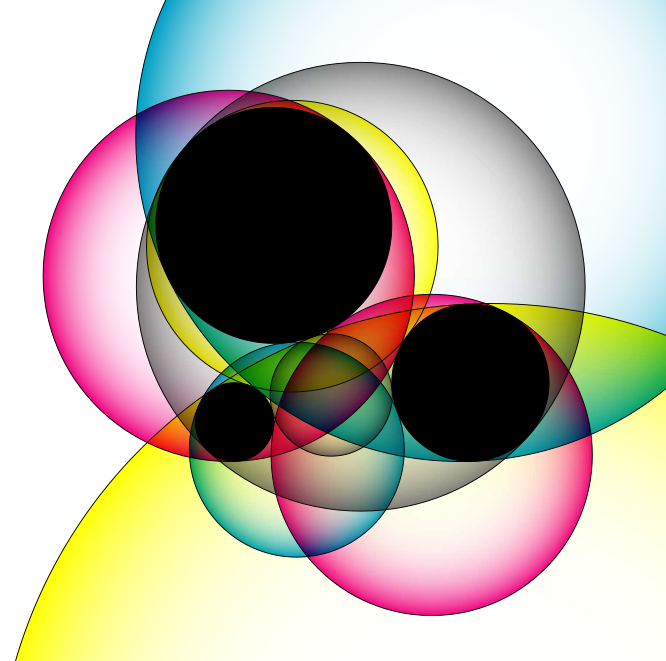
\includegraphics[width=4cm]{image/Appolonius.png}

        \section{Axiomes et notations}

%\addlb{[Peut-on supprimer l'espace entre "premières" et le point juste au dessus ?]} 

\begin{notion}
La construction axiomatique synthétique (à partir des points, des droites etc.) du plan euclidien consiste en ceci\,: on admet l'existence d'un ensemble appelé plan euclidien (qu'on notera $\mathcal{E}$), dont les éléments sont appelés points. On admet également l'existence d'un ensemble de sous-parties appelées droites (noté $\mathfrak{P}$). Le plan euclidien contient au moins une droite. 
\end{notion}

Les droites seront définies à travers les relations qu'elles entretiennent avec les points (axiomes d'incidence). Sur ces droites sont définies une notion d'ordonnancement à trois points caractérisée par les axiomes d'ordre, complétés par un axiome fort utile quand les points ne sont plus alignés : l'axiome de Pasch. Hilbert poursuit sa construction avec les axiomes dits de congruence concernant les règle de la relation du même nom. La congruence sous-tend, de façon synthétique, les notions de longueur et de mesure d'angle. Enfin, Hilbert introduit les axiomes de continuité qui vont caractériser les relations qu'entretiennent entre eux les points d'une droite quelquonque. Enfin l'axiome des parallèles est nécessaire afin de contraindre la géométrie a être Euclidienne. 

%Dans la suite on supposera connue la notion de longueur et nous construiront les notions d'angle et de mesure d'angle indépendamment des axiomes de congruence. 

 %On supposera connue la notions de distance entre points et rappellerons ceux des postulats d'Hilbert nécessaire à notre construction.

Dans la suite on notera les points (éléments de $\mathcal{E}$) en lettre latine majuscule ($A,B,C...$), les droites en lettre latine parenthésé minuscule ($(d),(e),(f)...$). 

%Ces axiomes peuvent se regrouper en cinq groupe. Le premier regroupes les axiomes d'incidences et décrit les relations d'appartenance entre points, droite et plan. Les axiomes d'ordres permettent de définir la relations "etre entre" et permettent de construire les notions de segment de demi-droit et de demi-plan. Les axiomes de congruences definissent la relations dites de congruences permettant de 

        \subsection{Axiomes d'incidences}\setcounter{serieaxiom}{1}\setcounter{axi}{0}

%\FigureMarge{Axiomes \ref{axi-A1} et \ref{axi-A2}}{image/axiome_d1.png}

%\marginnote{%
%    \tikzpicture[]
%        \node[text width=\marginparwidth, font=\small, align=center] (box) {Axiomes \ref{axi-A1} et \ref{axi-A2} \\ 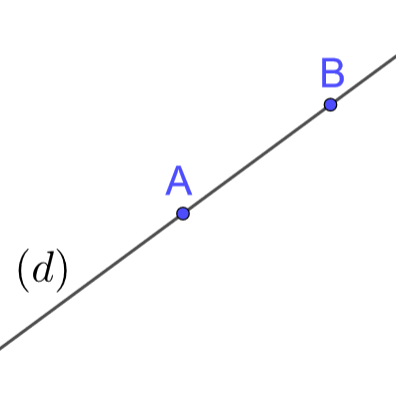
\includegraphics[width=0.7\marginparwidth]{image/axiome_d1.png}};
%\endtikzpicture
%}[0.0cm]

Hilbert commence par demander comme Euclide à ce qu'il ne passe qu'une droite entre deux points :
\FigureMarge{Axiomes \ref{axi-A1} et \ref{axi-A2}}{1.2}{image/axiome_d1.png}

\begin{axi}\label{axi-A1}
Soient $A$ et $B$ deux points distinct, il existe une unique droite $(d)$ contenant $A$ et $B$. On note $(AB)$ cette unique droite.  
    \begin{equation*}
        \forall A, B \in \mathcal{E},\, A,B \text{ distincts },\exists!(d), A,B\in(d)\,.
    \end{equation*}
\end{axi}
\begin{rema}
    De l'axiome \ref{axi-A1} on déduit que $(AB)=(BA)$. On déduit également que si $C$, distinct de $A$ et $B$, appartient également à $(d)$ alors $(d)=(AC)=(BC)=(AB)$. 
\end{rema}
L'axiome qui suit (Ax. \ref{axi-A2}) assure alors que toute droite contient au moins deux points sur une droite donnée. Ce genre de questionnement d'existence n'apparaît pas chez Euclide et y est supposé évident.
\begin{axi}\label{axi-A2}
    Soit une droite $(d)$, alors il existe au moins deux points sur cette droite.
    \begin{equation*}
        (d)\in\mathcal{D} \Rightarrow \exists A,B\in (d)\,.
    \end{equation*}
\end{axi}
De même l'axiome (Ax.\ref{axi-A3}), qui suit assure l'existence de points cette fois-ci en dehors d'une droite donnée. Cet axiome assure en quelque sorte que la dimension de l'espace est au moins deux. On conçoit donc qu'une axiomatisation de la droite et non du plan euclidien devra reconduire cette axiome. 
\FigureMarge{Axiome \ref{axi-A3} }{1}{image/axiome_d2.png}
\begin{axi}\label{axi-A3}
    Pour toute droite il existe au moins un point qui n'est pas sur cette droite. 
    \begin{equation*}
        \forall (d)\in \mathcal{D}\Rightarrow \exists A\in\mathcal{E}-(d)\,.
    \end{equation*}
\end{axi}
On l'a expliqué, l'axiome \ref{axi-A3} doit être enlevé si l'ont cherche à caractériser l'espace euclidien de dimension $1$. Ici on s'intéresse au plan euclidien, néanmoins pour pouvoir axiomatiser les espaces Euclidiens de dimensions $3$ ou plus, Hilbert adjoint à ces axiomes quatre autres axiomes d'incidence. Ceux-ci caractérisent les rapports d'appartenance des plans vis-à-vis des points et des droites. Ceci n'est pas notre propos\,: les angles ayant leurs existence dans les plans, l'ajout de ces axiomes est sans utilité dans notre construction. Nous les épargnerons donc au lecteur.
     
        \subsection{Axiomes d'ordre et axiomes de Pash}\setcounter{serieaxiom}{2}\setcounter{axi}{0}

Les axiomes d'ordre déterminent les règles d'emploi d'une relation ternaire importante entre triplet de points (alignés)\,:  la relation \guil{être entre}. Ces axiomes caractérisent les règles concernant la position relative des points sur une droite. Cette relation \guil{être entre} est nécessaire pour définir segment, demi-droite, demi-plan et secteur d'angle. Pour tout points $A,B$ et $C$ on lira $A\star B \star C$ : \guil{ $B$ est entre $A$ et $C$}.

Avant d'énoncer les axiome d'ordres donnons la définitions de l'alignement:
\begin{defi}[Points alignés]
    D'un ensemble de points distincts, on dit qu'ils sont alignés \ssi il existe une droite qui les contient tous. 
\end{defi}

\FigureMarge{Axiome \ref{ax-B1}}{1}{image/axiome_align1.png}


La première règle a imposer à la relation \guil{être entre} est qu'elle soit \guil{symétrique par rapport au point extérieur} et qu'elle impose aux trois points concerné d'être alignés\,: 



\begin{axi}\label{ax-B1}
    Soit $A,B$ et $C$ trois points tels que $A\star B \star C$, alors $A,B$ et $C$ sont trois points distincts, alignés et $C\star B \star A$.
    \begin{align*}
        \forall A,B,C\in&\mathcal{E},\, A,B,C \text{ distincts },  \\
        &\left(A\star B \star C\Rightarrow A,B,C \text{ alignés } \text{ et } C\star B \star A \right)\,.
    \end{align*}
\end{axi}
%\marginpar{\begin{center}Axiome \ref{ax-B2}\,:\\ 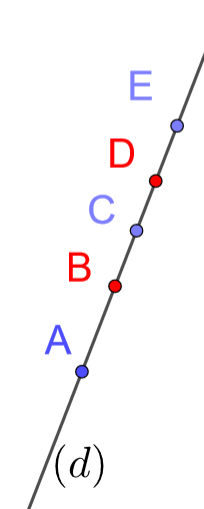
\includegraphics[width=0.35\marginparwidth]{image/axiome_align2.png}\end{center}}

\FigureMarge{Axiome \ref{ax-B2}}{1}{image/axiome_align2.png}


On se donne également l'existence de points entre et à l'\guil{extérieur} d'un couple de points donnés\,: 
\begin{axi}\label{ax-B2}
    Soit $B$ et $D$ deux points distincts, alors il existe des points $A,C$ et $E$ tel que $A\star B \star D$, $B\star C \star D$ et $B\star D \star E$.
    \begin{equation*}
        B,D\in\mathcal{E},\, B,D \text{ distincts } \Rightarrow \exists A,C,E\in\mathcal{E},\, A\star B \star D,\, B\star C \star D\,, B\star D \star E\,.
    \end{equation*}
\end{axi}
Enfin si l'on se donne trois points alignés, une relation \guil{être entre} existe entre ces trois point et è permutation des points extérieurs près, aucune autre relation de ce type n'est établie entre les trois points\,:
\begin{axi}\label{ax-B3}
    Pour trois points distincts sur une même droite, un et un seul est entre les deux autres.
\end{axi}
\begin{exo}
On suppose connues les notions ordinaires de géométrie euclidienne et on se demande si d'autres ensembles de parties peuvent satisfaire les axiomes d'ordre et de congruence. 

Soit $(d)$ une droite dans le plan euclidien, si on note $\mathfrak{C}$, l'ensemble des cercles dont le centre est contenu dans une droite $(d)$ et des droites orthogonales à $(d)$. Montrer que cet ensemble satisfait à tous les axiomes d'incidence (ou l'on remplace \guil{droite} par élément de $\mathfrak{C}$). Expliquer alors pourquoi la relation \guil{être entre} ne peux pas tenir ici.
\end{exo}
Le prochain axiome s'écrit plus aisément si on introduit la notion de segment ouvert\,: 
\begin{defi}[Segment]\label{defi-segment}
Soit $A$ et $B$ deux points distincts, alors on appelle segment ouvert d'extrémité $A$ et $B$ l'ensemble de points
\begin{equation*}
    ]AB[ = \ensemble{M\in\mathcal{E}}{A\star M \star B}\,.
\end{equation*}
De même on définit le segment fermé d'extrémité $A$ et $B$ l'ensemble de point
\begin{equation*}
    [AB] = ]AB[\cup \left\{A,B\right\}\,,
\end{equation*}
et les segments mixtes
\begin{equation*}
    ]AB] = ]AB[\cup \left\{B\right\},\qquad [AB[ = ]AB[\cup \left\{A\right\}\,.
\end{equation*}
\end{defi}
\begin{rema}
    De l'axiome \ref{ax-B1} on déduit que les segments ouverts et fermés sont \guil{non-ordonnés} : $]AB[=]BA[$ et $[AB]=[BA]$.
\end{rema}
L'axiome de Pasch caractérise le nombre d'intersections que fait une droite sécante avec les trois segments qu'on peut construire à l'aide de trois points\,: 
\setcounter{axi}{4}
\begin{axi}[Pasch]\label{ax-pasch}
    Soient trois points distincts et une droite contenue dans un plan tel qu'aucun des trois points n'appartiennent à la droite. Alors soit la droite ne rencontre aucun des segments ouvert formé par les trois points soit elle en rencontre deux (voir figure \ref{fig_pasch}).

    %Plus formellement si on note $\left(]s_i[\right)_{i=1,2,3}$ les trois segments ouverts formé par trois points et $(d)$ une droite ne passant par aucun des trois plan et contenue dans un plan contenant les trois points (et donc également les segments) alors,
    %\begin{equation*}
        %\sum_{i=1,2,3}\mathbf{Card}\left((d)\cap]s_i[\right) = 0 \text{ où } 2\,.
    %\end{equation*}
\end{axi}
\begin{rema}
    Une lecture hâtive de cet axiome peut induire le lecteur en erreur. Le contresens possible est le suivant. Si l'on conçoit un triangle comme la réunion des segments ouverts qui le constituent, alors l'intersection d'un triangle avec une droite est soit vide soit constituée de deux points. L'erreur est ici de n'avoir pas pris en considération les triangles \guil{plats}. Dans ce cas l'intersection avec la réunions des segments ouvert peut être constitué d'un seul point. Et pourtant la droite rencontre deux des segments (l'un est inclus dans l'autre).
\end{rema}
\begin{figure}[h!]
    \centering
    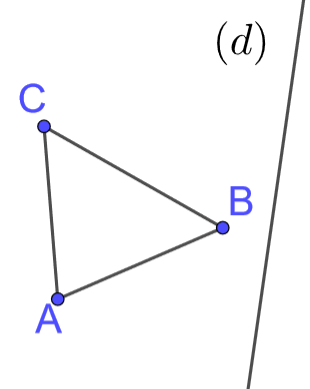
\includegraphics[width=0.3\textwidth]{image/axiome_pasch1.png}\hfill
    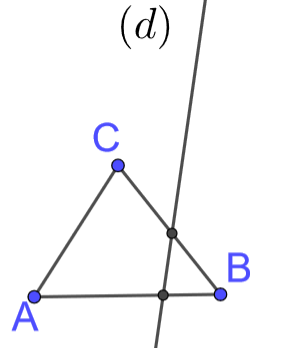
\includegraphics[width=0.3\textwidth]{image/axiome_pasch2.png}
    \caption{Illustration de l'axiome \ref{ax-pasch}. À gauche\,: pas d'intersection. À droite\,: deux intersections. Ne pas oublier que l'axiome interdit que la droite passe par l'un des trois points $A,B$ ou $C$.}
    \label{fig_pasch}
\end{figure}
Le lecteur attentif aura remarqué l'absence de l'axiome B.4. Hilbert l'introduit dans son article original. Cet axiome caractérise les relations \guil{être entre} possibles quand quatre points distincts appartiennent à une même droite. Cet axiome est redondant. C'est-à-dire qu'il peut être démontré à partir des axiomes d'incidence et d'ordre. Pour être tout à fait exact il est redondant si l'axiome de Pasch est formulé en intégrant le cas des triplets de points alignés (comme on l'a fait ici ou dans la publication de Hilbert). La \href{https://www.ams.org/journals/tran/1902-003-01/S0002-9947-1902-1500592-8/S0002-9947-1902-1500592-8.pdf}{preuve} de cette redondance axiomatique est due à Eliakim Hastings et Robert Lee Moore \cite{moore1902projective}, deux mathématiciens Américains homonymes. La preuve est fondée sur quelques lemmes concernant les quadruplets de points alignés dont la preuve repose sur la configuration alignée de l'axiome de Pasch. Ces lemmes nous seront fort utiles et sont présenté en sous-section \ref{subsec-quatrepoints}. L'axiome redondant en question ne nous sera pas utiles. %\addlb{[Ça représente tout de même des pages de démonstrations dans ton bazar...]}

        \subsection{Axiomes de congruences}\setcounter{axi}{0}\setcounter{serieaxiom}{3}

Les axiomes de congruence définissent trois relations dites de congruence entre segments, entre secteurs d'angles ou entre triangles (ces notions sont définies plus loin). Quelques soit le type d'objet considéré (segments, secteurs d'angles et triangles) on notera $\equiv$ la relation de congruence entre deux objets de même nature.

%Une fois les axiomes énumérés, on montrera qu'ils correspondent à l'égalité de mesures des segments (autrement dit, l'isométrie). Cela sera fort utile pour établir des relations entre les mesures d'angles dans la section \ref{subsec_secang}.

Le premier axiome de congruence utilise la notion de demi-droite, ces parties du plan sont definies ainsi\,:
\begin{defi}[Demi-droite]\label{def-demidroite}
    Soit $A$ et $B$ deux points distincts, alors on appelle demi-droite ouverte d'extrémité $A$ contenant $B$ l'ensemble,
    \begin{equation*}
        ]AB) = ]AB] \cup \ensemble{M\in\mathcal{E}}{A\star B \star M}\,.
    \end{equation*}
    et on appelle demi droite fermée d'extrémité $A$ et contenant $B$ l'ensemble,
    \begin{equation*}
        [AB) = ]AB) \cup \left\{A\right\}\,.
    \end{equation*}

    Un ensemble $]d)$ (respectivement $[d)$) est une demi-droite ouverte (respectivement fermé) \ssi il existe $A$ et $B$ distincts tels que $]d)=]AB)$ (respectivement $[d)=[AB)$). On appelle alors $(d)=(AB)$ la droite support des demi-droites $]AB)$ et $[AB)$. 
\end{defi}
\begin{rema}
    Par construction il existe une unique demi-droite (ouverte ou fermée) d'extrémité donnée passant par un point distinct de l'extrémité.
\end{rema}
Le premier axiome pourrait s'appeler axiome du compas, il signifie qu'on peut toujours reporter un segment sur une demi-droite en partant d'une de ses extrémités. Hilbert travaillera avec une droite et définira deux reports possibles. On préfère, pour plus de simplicité par la suite travailler directement avec des demi-droites.
\begin{axi}\label{axi-C1}
    Soit $A$ et $B$ deux points distinct et $]d)$ une demi-droite ouverte d'extrémité $A'$. Alors il existe un unique point $B'$ dans $]d)$ tel que $[AB]$ soit congru à $[A'B']$.
    \begin{align*}
        \forall A,B\in\mathcal{E}, A\neq B,\, \forall ]d) &\text{ demi-droite d'extrémité } A',\, \\
        &\Rightarrow \exists ! B'\in ]d)\,, [AB] \equiv [A'B']\,.
    \end{align*}
\end{axi}
\FigureMarge{Axiome \ref{axi-C1}}{1.2}{image/Axiome_C1.png}
Il paraît conséquent de demander qu'un segment puisse être reporté sur lui-même. De même que si l'un peut être reporté sur le second et que le second peut être reporté sur le troisième alors le premier peut être reporté sur le troisième.
\begin{axi}\label{axi-C2}
    La relation de congruence entre segments est réflexive et transitive.
\end{axi}
\begin{rema} (Rappel)
Une relation binaire $\sim$ sur un ensemble $E$ est une partie de $E\times E$. Plus familièrement deux éléments $x$ et $y$ dans $E$ peuvent être ou ne pas être en relation. Si on note $\sim$ la relation, on notera $x \sim y$ pour signifier\,: \guil{$x$ est en relation avec $y$}. Par exemple pour l'ensemble $\mathfrak{D}$ on peut définir la relation \guil{est parallèle à}. Une relation est dite relation d'équivalence \ssi $\forall x,y,z\in E$\,:
\begin{itemize}[$\bullet$]
    \item elle est symétrique\,:  $x\sim y \Rightarrow y \sim x$,
    \item elle est réflexive\,: $x\sim x$,
    \item et elle est transitive\,:$((x\sim y)\wedge (y\sim z)) \Rightarrow x\sim z$.
\end{itemize}
On vérifie facilement que la relation \guil{est parallèle à} est une relation d'équivalence.
\end{rema}
\begin{rema}
    On peut montrer que $\equiv$ est symétrique. Ainsi, on a le théorème suivant\,:
\end{rema}
\begin{thm}\label{thm-congsegmentequiv}
    La relation de congruence entre segments est une relation d'équivalence.
\begin{proof}
    Il suffit de prouver la symétrie de la relation de congruence entre segments. Soit $A,B,A'$ et $B'$ quatre points tel que $A$ soit distinct de $B$, $A'$ soit distinct de $B'$ et que $[AB]\equiv[A'B']$. On note $]d)=]AB)$. 
    
    L'axiome \ref{axi-C1} implique l'existence d'un point $B''$ sur $]d)$ tel que $[A'B']\equiv[AB'']$. La transitivité (Ax.\ref{axi-C2}) assure,
    \begin{equation*}
        \left\{
        \begin{array}{cc}
             \left[AB\right]&\equiv\left[A'B'\right]  \\
             \left[A'B'\right]&\equiv\left[AB''\right]
        \end{array}
        \right.\quad \Longrightarrow \quad [AB]\equiv[AB'']\,.
    \end{equation*}
    
    Par réflexivité de la relation de congruence entre segment (Ax.\ref{axi-C2}) on a $[AB]\equiv[AB]$, ainsi $B$ et $B''$ sont deux point de la demi-droite $[d)$ d'extrémité $A$ tel que,
    \begin{equation*}
        \left\{
        \begin{array}{cc}
             \left[AB\right]& \equiv \left[AB''\right]  \\
             \left[AB\right]&\equiv \left[AB \right]
        \end{array}
        \right.\,.
    \end{equation*}
    
    Par unicité dans l'axiome \ref{axi-C1} les congruences précédentes assurent $B''=B$ et donc $[A'B']\equiv[AB'']$ devient,
    \begin{equation*}
        [A'B']\equiv[AB]\,,
    \end{equation*}
    ce qui prouve la symétrie de $\equiv$ sur les segments. 
\end{proof}
\end{thm}
La congruence entre segments doit traduire la notion de longueur. Il apparaît alors essentiel d'assurer une forme d'additivité des longueurs sur des points alignés. Cela se traduira par\,:
\begin{axi}\label{axi-C3}
    Soit $(d)$ et $(d')$ deux droites et $A,B,C \in (d)$ tels que $A \star B \star C$ et $A',B',C' \in (d')$ tels que $A' \star B' \star C'$. Alors si $[AB]$ et congru à $[A'B']$ et $[BC]$ et congru à $[B'C']$ alors $[AC]$ et congru à $[A'C']$.
\end{axi}   
\FigureMarge{Axiome \ref{axi-C3}}{1.2}{image/Axiome_C3.png}
Le prochain axiome de congruence traitera de la congruence entre secteurs d'angle saillants. Les secteurs d'angle saillants sont des portions du plan reposant sur la notion de demi-plan\,: 
\begin{defi}[Côtés d'une droite et demi-plan]\label{def-demiplan}
Soit $(d)$ une droite, $A$ et $B$ deux points de $\mathcal{E}$. Alors :
\begin{itemize}[$\bullet$]
    \item Soit $[AB]\cap (d) = \varnothing$ et on dit que $A$ et $B$ \emph{se situent du même côté} de $(d)$.
    \item Soit (exclusif) c'est que $[AB]\cap (d) \neq \varnothing$ et on dit que $A$ et $B$ \emph{se situent de part et d'autre} de $(d)$.
\end{itemize}
On appelle \emph{demi-plan} $\mathcal{P}_{(d),A}$ l'ensemble des points $M$ du plan tel que $M$ et $A$ se situant du même côté de $(d)$. La droite $(d)$ est alors appelé \emph{droite support} du demi plan $\mathcal{P}_{(d),A}$.
\end{defi}
\FigureMarge{Demi-plan \ref{def-demiplan}}{1.2}{image/DemiPlanDefPoint.png}
Une fois définie les demi-plans on peut définir les secteurs d'angle saillant\,: 
\begin{defi}[Secteur d'angle saillant]\label{defi-anglesaillant}
    Soit $I, O$ et $J$ trois points distincts et non alignés, alors on appelle secteur d'\emph{angle saillant} de sommet $O$ entre $]OI)$ et $]OJ)$ l'ensemble des points $M$ tel que $M$ et $J$ soit du même côté de $(OI)$ et que $M$ et $I$ sont du même côté de $(OJ)$. On note alors,
    \begin{equation*}
        \anglesaillant\left({O},{]OI)},{]OJ)}\right) := \mathcal{P}_{(OI),J} \cap \mathcal{P}_{(OJ),I}  
    \end{equation*}
    cet ensemble. %\addlb{[il faudra préciser dans l'intro qu'on note $:=$ les définitions.]}
\end{defi}
\FigureMarge{Secteur d'angle \\ saillant \ref{defi-anglesaillant}}{1.2}{image/SecteurSaillant3ptClair.png}
C'est sur ces ensembles que se définit la prochaine congruence. On demande qu'il n'existe qu'un report de secteur d'angle à partir d'une demi-droite donnée et d'un des demi-plan qu'elle supporte. 
\begin{axi}\label{axi-C4}
    Soient $]d_I)$ et $]d_J)$ deux demi-droites de même extrémité $O$. Soit $]d_I)'$ une demi-droite d'extrémité $O'$ dont la droite support est également celle d'un demi-plan $\mathcal{P}'$, alors il existe une unique demi-droite $]d_J')$ dans $\mathcal{P}'$ d'extrémité $O'$ tel que\,:
    $$\anglesaillant\left(O,]d_I),]d_J)\right)\equiv\anglesaillant\left(O',]d_I'),]d_J')\right)\,.$$
\end{axi}
\FigureMarge{Axiome \ref{axi-C4}}{1.2}{image/Axiome_C4}
Comme pour l'axiome \ref{axi-C1} Hilbert ne precise pas le demi-plan ou on cherche $]d_J')$, il préfère dire qu'il y en a deux. Nous préférons axiomatiser l'unicité par demi-plan afin de s'épargner une lourdeur dans la rédaction des preuves qui suivront. 
\begin{axi}\label{axi-C5}
    La relation de congruence entre angles est transitive et réflexive. 
\end{axi}
On montre de même que pour les segments, que la relation de congruence pour les secteurs d'angles est une relation d'équivalence.
\begin{thm}
    La relation de congruence entre secteurs d'angle est une relation d'équivalence.
\begin{proof}
    La preuve s'effectue de la même manière que celles du théorème \ref{thm-congsegmentequiv}.
\end{proof}
\end{thm}
La prochaine relation d'équivalence concerne les triangles, on définira ces objets \guil{bien connus} comme une suite ordonnée de trois points distincts. 
\begin{defi}[Triangle]
    On appelle \emph{triangle} la donnée de trois points distincts \emph{ordonnées}. Ces points sont appelés sommets du triangle.
\end{defi}
\begin{defi}[Secteur d'angle au sommet d'un triangle]
    Soit $A,B$ et $C$ trois points distincts, on appelle secteurs d'angles du sommet $A$ dans le triangle $ABC$ le secteurs d'angle,
    \begin{equation*}
        \anglesaillant\left(A,]AB),]AC)\right)\,.
    \end{equation*}
\end{defi}
Cette fois-ci cependant la nouvelle congruence (entre triangle) peut être définie positivement, \cad en faisant appelle a des notions déjà connues. 
\begin{defi}[Congruence entre triangles]
    Deux triangles $ABC$ et $A'B'C'$ sont dit congruents \ssi :
    \begin{equation*}
        \left\{
        \begin{array}{ccc}
            [AB] \equiv [A'B']\,, &&  \anglesaillant\left(C,]CA),]CB)\right)\equiv \anglesaillant\left(C',]C'A'),]C'B')\right) \\
            \left[BC\right] \equiv \left[B'C'\right] \,, && \anglesaillant\left(A,]AB),]AC)\right)\equiv \anglesaillant\left(A',]A'B'),]A'C')\right) \\
            \left[CA\right] \equiv \left[C'A'\right]\,, && \anglesaillant\left(B,]BA),]BC)\right)\equiv \anglesaillant\left(B',]B'A'),]B'C')\right)
        \end{array}
        \right.
    \end{equation*}
Autrement dit si tout \guil{leurs angles} et tous leurs \guil{segments} sont congruent deux-à-deux.
\end{defi}
\begin{rema}
    L'ordre des points d'un triangle compte ! En effet si $ABC\equiv A'B'C'$ cela n'implique pas $ABD\equiv B'C'A'$. En effet les congruence à vérifier deux à deux sont déterminées par l'ordre des points. En général $ABC \not \equiv BCA$. 
\end{rema}
\begin{rema}
    Soit $ABC$ un triangle vérifiant $ABC \equiv CBA$ alors ce triangle est isocèle en $B$.
\end{rema}
Il semble que les six congruences à vérifier soient de trop. En effet d'instinct on pense par exemple que si les trois relations de congruence entre segments sont vérifiées, alors il en est de même pour les secteurs d'angle. De même pour un angle et ses côtés adjacents. Ces résultats qualifiés de \guil{cas d'égalité du triangle} ne sont pas démontrables en l'état. Euclide fournit une démonstration bancale de premier cas d'égalité, les autres se déduisant à partir du premier étant correct. Ces cas d'égalités des triangle peuvent être vus comme théorèmes pivots de la géométrie euclidienne. Ne pouvant démontrer rigoureusement le premier, Hilbert en fait un axiome.    
\begin{axi}\label{axi-C6}
    Si deux triangles ont chacun un angle au sommet et les côtés adjacents à ce sommet reliés par une congruence, alors ils sont congruents.
    Autrement dit, si $A_1B_1C_1$ et $A_2B_2C_2$ sont deux triangles tels que les angles aux sommets $A_1$ et $A_2$ sont congruents, alors\,:
    \begin{equation*}
        A_1B_1C_1\equiv A_2B_2C_2\Leftrightarrow((A_1B_1\equiv A_2B_2)\wedge (A_1C_1\equiv A_2C_2))
    \end{equation*}
\end{axi}
\FigureMarge{Axiome \ref{axi-C6}\,: on a codé\\ la congruence de paires\\ d'objets à l'aide\\ des couleurs.}{1.2}{image/tri_cong.png}
%\marginpar{\begin{center}Axiome \ref{axi-C6}\,: on a codé\\ la congruence de paires\\ d'objets à l'aide\\ des couleurs.\\
%    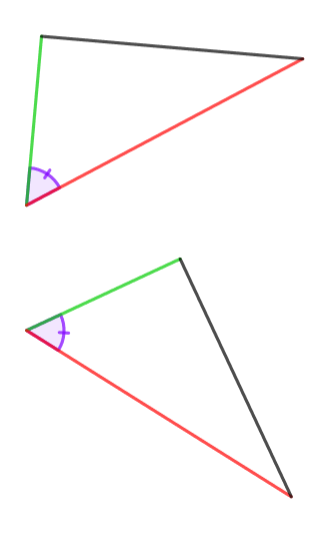
\includegraphics[width=0.5\marginparwidth]{image/tri_cong.png}
%\end{center}}

        \subsection{Axiomes de continuité}\setcounter{axi}{0}\setcounter{serieaxiom}{4}

Les axiomes de continuité vont assurer des propriétés concernant les relations que les points entretiennent entre eux dans l'espace. En particulier, on assurera qu'il est possible de dépasser en taille n'importe quel segment à partir d'un autre, en le reportant un nombre de fois arbitrairement grand.
\begin{defi}[Report]
    Soit $[AB]$ un segment et $]d)$ un demi-droite d'extremité $O$, on appelle report de $[AB]$ sur $]d)$ l'unique point $C$ de $]d)$ tel que $[OC]\equiv [AB]$.
\end{defi}
\begin{rema}
    Par construction le report de $[AB]$ sur $]d)$ est distinct de $O$. 
\end{rema}
Par la suite il sera utile d'établir les résultats suivants.
\begin{prop}
Pour tout points $A$ et $B$ distincts, l'ensemble,
\begin{equation*}
    \ensemble{M\in \mathcal{E}}{A\star B\star M}
\end{equation*}
est une demi-droite d'extrémité $B$.
\begin{proof}
    \addlb{[remarque : pour que tes preuves soient plus lisibles, ne suppose pas que tes lecteurs ont lu 8000 fois ton texte (comme toi) et connaissent par coeur les numéros des théorèmes. Ajoute au moins un petit nom pour rappeler de quoi tu parle. C'est ultra chiant de naviguer en permanence pour se rappeler ce que signifie "axiome B2", "corrolaire 6.2.2" etc.]}

    
    Notons abusivement $]d)$ l'ensemble en question. Soit $C$ dans $]d)$ (existence assuré par l'axiome \ref{ax-B2}). Alors $A\star B\star C$. Le but est alors de montrer que $]d)=]BC)$. 

    Soit $M\in ]d)$ alors on à $A\star B\star M$ et $A\star B\star C$. Si $M=C$ puisque $C\in ]BC)$ sinon on utilise le corollaire \ref{cor-configurationuncote} (dont la démonstration, on l'assure, ne repose que sur les axiomes d'incidence et d'ordre). Ce corollaire assure alors que $B\star M \star C$ (\cad $M\in]AC]$) où $B\star C\star M$ autrement dit $M\in ]BC)$. On en déduit $]d)\subset ]BC)$.

    Soit $M\in ]BC)$ et donc \,:
    \begin{itemize}[$\bullet$]
        \item soit $M=C$ et donc $M \in ]d)$,
        \item soit $M\in ]BC[$ et donc $B\star M\star C$, ce qui, combiné au fait que $A\star B\star C$ conduit d'après le Corollaire.\ref{cor-configurationordrequatrepoint-1} (dont la démonstration, on l'assure, ne repose que sur les axiomes d'incidence et d'ordre) à $A\star B \star M$ et donc $M\in ]d)$.
        \item soit $B \star M \star C$, ce qui combiné au fait que $A\star B\star C$ conduit d'après le Corollaire.\ref{cor-configurationordrequatrepoint-2} (dont la démonstration, on l'assure, ne repose que sur les axiomes d'incidence et d'ordre) à $A\star B \star M$ et donc $M\in ]d)$.
    \end{itemize}
    Dans tout les cas $M\in ]d)$ et donc $]BC)\subset ]d)$.
\end{proof}
\end{prop}
On en déduit en combinant cette proposition avec l'axiome de congruence \ref{axi-C1} que,
\begin{prop}
    Pour tout points $A$ et $B$ distincts et tout segment $[CD]$, il existe un unique point $M$ tel que $A\star B \star M$ et $[CD]\equiv [BM]$. 
\begin{proof}
    Immédiat.
\end{proof}
\end{prop}

On définit alors pour tout $n$ le $n$-report de $[AB]$ sur $]d)$:
\begin{defi}[$n$-Report]
    Soit $[AB]$ un segment, $]d)$ une demi-droite d'extrémité $O$. On construit alors par récurrence la suite de point $\famiin{C}{k}{\N}$ :
    \begin{equation*}
        \left\{\begin{array}{rl}
             C_0 & = O\\
             C_1 & \text{est le report de $[AB]$ sur $]d)$} \\% et $]d_1)$ l'unique demi-droite d'extrémité $C_1$ incluse dans $]d)$}  \\
             C_{n+1} & \text{est l'unique point de $(AB)$ tel que $O\star C_n \star C_{n+1}$ et $[C_n C_{n+1}]\equiv [AB]$}
        \end{array}
        \right.
    \end{equation*}
    Alors pour tout $n\in \N$, le point $C_n$ est appelé $n$-report de $[AB]$ sur $]d)$.
\end{defi}

\begin{rema}
    \added[id=LB]{Ici, on parle de suite (qui plus est, définie par récurrence), alors qu'à aucun moment on n'a expliqué ce que c'était au lecteur. Notre cours est donc incompréhensible.}
\end{rema}

\begin{rema}
    Cette relation de récurrence est bien définie. En effet pour tout $O,C$ deux points distincts, il n'existe qu'une demi-droite d'extrémité $C$ ne contenant pas $O$, cela est une conséquences de l'axiome \ref{axi-A3}. 
\end{rema}
\begin{rema}
    Dans la suite dans le cas ou $O=A$ et $B\in ]d)$ on notera $A+n\overrightarrow{AB}$ le $n$-report de $[AB]$ sur $[AB)$.
\end{rema}
Ces notions vont permettre de formaliser l'axiome d'Archimède. 
\begin{axi}[Archimède]\label{axi-archimede}
    Soit $[AB]$ et $[CD]$ deux segments alors il existe un entier $n$ tel que $E$, le $n$-report de $[CD]$ sur $[AB)$ vérifie $A\star B \star E$. 
\end{axi}

Dans la suite de cette section, on notera,
\begin{equation*}
    \D_+ = \ensemble{\dfrac{n}{2^k}}{(n,k)\in \N_\star\times\N }
\end{equation*}
\addlb{Vu qu'on n'a jamais parlé de produit cartésien, il vaut mieux bannir cette notation et mettre $n\in\N_\star, k\in\N$.}
l'ensemble des nombre diadique. Dans la logique de Dedekind, on rappelle (ou pas) que pour toute partition,
\begin{equation*}
    \D_1 \cap \D_2 = \D_+ 
\end{equation*}
non vide de $\D_+$, telle que,
\begin{equation*}
    \forall (d_1,d_2)\in \D_1 \times \D_2\,, \text{ on ai } d_1 < d_1
\end{equation*}
il existe un unique nombre réel $x\in \R_+^\star$ tel que,
\begin{equation*}
    \forall (d_1,d_2)\in \D_1 \times \D_2\,, \text{ on ai } d_1 \leq x \leq d_1\,.
\end{equation*}
$x$ est alors le plus petit majorant de $\D_1$ ou symétriquement le plus grand majorant de $\D_2$. 

Les axiomes précédent ne sont pas suffisants pour assurer que l'espace \guil{ne contient pas de trou} (voir Exo. \ref{exo-constructible}). L'axiome suivant assurera alors à l'espace cette propriété. 
\begin{axi}[Dedekind]\label{axi-dedekind}
    Soit $]d)$ une demi-droite ouvert d'extrémité $O$ qui est la partition en deux ensemble $\Sigma_-$ et $\Sigma_+$ et tel que $\forall (A_-,A_+)\in \Sigma_-\times \Sigma_+$ on ai $O\star A_- \star A_+$. Alors il existe un unique point $X$ tel que $\forall (A_-,A_+)\in \Sigma_-\times \Sigma_+$ on ai $ A_- \star X \star A_+$.
\end{axi}
Hilbert n'énonce pas cet axiome et préfère énoncer un axiome équivalent dit de l'intégrité linéaire. 

Néanmoins sa formulation \guil{méta} nous a conduit a préféré cette formulation. 
\addlb{[incompréhensible et (donc) inutile si tu ne cites pas ledit axiome. Je propose de supprimer cette remarque.]}

\begin{exo}\label{exo-constructible}
On se place dans $\R^2$ \addlb{On n'a jamais défini $\R^2$!!!}, et on cherche a savoir si la sous-partie des points dit constructible peut satisfaire à tout les axiomes de Hilbert. 

Les points dit constructibles sont définis comme points issus d'une succession finie d'étapes\addlb{, \guil{à la règle non graduée et au compas}, c'est-à-dire de la manière suivante}. Soit une sous partie $E\subset \R^2$, on dit qu'un point $M$ est constructible \emph{en une étape} a partir de $E$ \ssi $M\in E$ ou si $E$ est l'intersection de partie du type :
\begin{itemize}[$\bullet$]
    \item un droite définie par deux points distincts de $E$\,;
    \item un cercle dont le centre est dans $E$ est dont le rayon est un segment formé par deux point distincts de $E$\,
\end{itemize} 
On note alors $\mathfrak{T}_1\left(E\right)$ l'ensemble des points contructibles à partir de $E$. On a bien évidement $E\subset \mathfrak{T}\left(E\right)$. On étend alors par récurrence $\mathfrak{T}_{n+1}\left(E\right):=\mathfrak{T}_1\left(\mathfrak{T}_n\left(E\right)\right)$ l'ensemble des points constructibles en $n$ étapes à partir de $E$. Enfin on définit l'ensemble des nombres constructibles à partir de $E$ comme l'ensemble des points $M$ tel qu'il existe $n\in\N$ tel que $M\in \mathfrak{T}_n\left(E\right)$ et on notera $\mathcal{T}\left(E\right)$ l'ensemble des points constructibles à partir de $E$.

On se donne deux points distincts $O=(0,0)$ et $I=(0,1)$ et on note $\mathfrak{T}\left(\{O,I\}\right)=\mathfrak{T}$
\begin{enumerate}
    \item Discuter du fait que $\Z^2 \subset \mathfrak{T}$.
    \item De même argumenter $\Q^2 \subset \mathfrak{T}$.
    \item Montrer que $\mathfrak{T}$ est strictement plus grand que $\Q^2$. \addlb{[définis "plus grand que".]}
    \item $\mathfrak{T}$ respecte-t-il tout les axiomes de Hilbert (a l'exception de l'axiome de Dedekind)? 
    \item Sachant que $(\pi,0)\notin \mathfrak{T}$ en déduire que $\mathfrak{T}$ ne respecte pas l'axiome de Dedekind. 
\end{enumerate}
\end{exo}

        \subsection{Axiome des parallèles}

Enfin il y a l'axiome qui a été le plus discuté\,: l'axiome des parallèles.

\begin{defi}[Droites parallèles]
    Deux droites $(d_1)$ et $(d_2)$ sont \emph{parallèles} \ssi $(d_1)\cap (d_2) = \varnothing$. On note alors $(d_1)\|(d_2)$. 
\end{defi}        
\begin{defi}[Droites sécantes]\label{def-secantes}
    Deux droites distinctes sont dites \emph{sécantes} \ssi leurs intersection est non vide.
\end{defi}
\begin{thm}[Droites sécantes]\label{thm-droitesecante}
    L'intersection deux deux droites sécantes est réduite à un point.
\end{thm}
\begin{proof}
    Si cette intersection étais composé de plus d'un point alors l'axiome (\ref{axi-A1}) impliquerait que ces deux droites soient identiques\,: non distinctes. Contradiction.
\end{proof}
\begin{axi}[Des parallèle]\label{axi-parra}
    Pour toute droite $(d)$ et pour tout point $P$ de $\mathcal{E}-(d)$ il existe une unique droite $(d')$ parallèle à $(d)$ et contenant $P$.
\end{axi}

L'exposé des axiomes est terminé. Il est maintenant temps de s'attaquer à ces longues chaînes de raisons qui donnaient a Descartes l'idée\guil{que toutes les choses qui peuvent tomber sous la connaissance des hommes s'entresuivent en même façon}.

%\epigraph{Ces longues chaînes de raison, si simples et faciles, dont les géomètres ont coutume de se servir pour parvenir à leurs plus difficiles démonstrations, m'avaient donné occasion de m'imaginer que toutes les choses qui peuvent tomber sous la connaissance des hommes s'entresuivent en même façon.}{Descartes, Discours de la méthode.}

    \section{Résultats et constructions préalables}
    \addlb{[Ce titre sent le moisi.]}

    L'objet de cette section est d'établir quelques résultats relativement proches des axiomes et qui nous serviront tout aux long du chapitre \ref{chap_angle}.

    \addlb{[Ici tu répètes exactement ce que dit le titre... ça ne nous avance pas.]}


        \subsection{Résultat sur l'ordonnancement de quatre points}\label{subsec-quatrepoints}


\replaced[id=LB]{Cette partie contient}{Les résultats de cette partie concernent} des résultats primordiaux sur l'ordonnancement à quatre points. Énoncés extrêmement évidents sur des dessins, leurs démonstration à partir des axiomes est laborieuse. Nous conseillons aux lecteurs de passer les démonstrations et de lire néanmoins les énoncés des lemmes et corollaires en première lecture.  Ces résultats sont les fondations de la \href{https://www.ams.org/journals/tran/1902-003-01/S0002-9947-1902-1500592-8/S0002-9947-1902-1500592-8.pdf}{preuve}\footnote{\url{https://www.ams.org/journals/tran/1902-003-01/S0002-9947-1902-1500592-8/S0002-9947-1902-1500592-8.pdf}} de l'\guil{axiome B4} par les américains Hastings Moore et Robert Lee Moore\,\cite{moore1902projective}. Les lemmes y démontrent des suites d'alignements impossibles en vertu de la configuration plate de l'axiome de Pasch (Ax. \ref{ax-pasch}). Les corollaires énoncent les déductions qui serviront dans des cas plus pratiques.

%\footnote{\url{https://www.ams.org/journals/tran/1902-003-01/S0002-9947-1902-1500592-8/S0002-9947-1902-1500592-8.pdf}}
    %Le lecteur attentif aura remarqué l'absence de l'axiome B.4. Dans son article original, Hilbert ajoute un quatrième axiome qui est en fait redondant, \cad qu'il peut être démontré à l'aides des axiomes (de \ref{axi-A1} à \ref{axi-A3} et \ref{ax-B1},\ref{ax-B2} et \ref{ax-pasch}). Pour être tout-à-fait exact, il est redondant si l'axiome de Pasch est formulé en intégrant le cas des triplets de points alignés (comme on l'a fait ici ou dans la publication de Hilbert). La \href{https://www.ams.org/journals/tran/1902-003-01/S0002-9947-1902-1500592-8/S0002-9947-1902-1500592-8.pdf}{preuve} de cette redondance axiomatique est due à Eliakim Hastings Moore et Robert Lee Moore deux mathématiciens Américains homonyme. La preuve est fondée sur quelques Lemme concernant les quadruplets de points alignés. La preuve de ces lemmes repose sur la configuration alignée des trois points de l'axiome de Pasch.

    %Nous ne présenterons ici certains des lemmes intervenants dans cette preuve car ils s'avèrent utile dans le reste de notre contruction. Il pourra sembler au lecteur que nous prouvons ici des évidences. La lecture des preuve pourra être passée en première lecture, elle offre néanmoins une jolie illustration de la puissance de l'axiome de Pash.

\begin{lem}[Impossibilité cyclique]\label{lem-Impossibilitecyclique}
    Soit $\fami{A}{i}{1,2,3,4}$ quatre points distincts appartenant à une même droite. Alors les systèmes de relation, dit cycliques et pseudo-cycliques,
        \begin{equation*}
        \left\{
            \begin{array}{c}
                 A_{1} \star A_{2} \star A_{3} \\
                 A_{2} \star A_{3} \star A_{4}\\
                 A_{3} \star A_{4} \star A_{1}\\
            \end{array}
            \right. 
             \quad\text{ ou }\qquad \left\{
            \begin{array}{c}
                 A_{1} \star A_{2} \star A_{3} \\
                 A_{2} \star A_{3} \star A_{4}\\
                 A_{4} \star A_{1} \star A_{3}\\
            \end{array}
            \right.
            \,.
    \end{equation*}
    sont impossibles. 
    \begin{proof}
        Les deux premières relations des deux systèmes sont les même. On commencera par supposer vraies uniquement ces deux première relations.
    
        Notons $(d_s)=(A_i A_j)$ pour $i\neq j = 1,2,3,4$, $]s_1[=]A_2 A_4[$, $]s_2[=]A_1 A_2[$ et enfin $]s_3[=]A_1 A_4[$. 

        L'axiome \ref{axi-A3} permet alors l'existence d'un point en dehors de $(d_s)$. On note $(d)=(A_3 A)$.  Par construction $(d)$ et $(d_s)$ sont sécantes d'intersection $B_3$.

        Puisque $A_{2} \star A_{3} \star A_{4}$, $A_3\in ]s_1[$ et donc $(d)\cap ]s_1[$ vaut $A_3$ car il contient $A_3$ et qu'il est composé d'au plus un point puisque inclus dans l'intersection des droites sécantes $(d)$ et $(d_s)$. Son cardinal est égal à $1$.

        $A_3 \notin ]s_2[ = ]A_1 A_2[$ car si c'était le cas, cela impliquerai $A_1 \star A_3 \star A_2$ qui est (en vertu de l'axiome \ref{ax-B3}) en contradiction avec $A_{1} \star A_{2} \star A_{3}$. Le cardinal de $(d)\cap]s_2[$ est donc $0$.

        La droite $(d)$ n'étant pas confondus avec $(d_s)$ est n'est pas confondus avec aucune des droites supports des segments ouverts $]s_1[,]s_2[$ et $]s_3[$. \addlb{Retravaille la syntaxe, la phrase précédente n'a aucun sens.}

        De plus $(d)$ ne passe ni par $A_1,A_2$ ou $A_4$ puisque vu que les points $\fami{A}{i}{1,2,3,4}$ sont distincts cela impliquerait que $(d)$ et $(d_s)$ soient confondues ce qui est exclu par construction de $(d)$.

        On peut donc appliquer l'axiome de Pasch \ref{ax-pasch} au triplet $A_1,A_2$ et $A_4$ et à la droite $(d)$. On en déduit que,
        \begin{equation*}
            (d)\cap]s_3[\neq \varnothing\,.
        \end{equation*}
        Or puisque $(d)\cap]s_3[ \subset (d)\cap (d_s) = \left\{B_3 \right\}$ et donc $(d)\cap]s_3[ = \left\{B_3 \right\}$ ce qui implique que $B_3 \in ]s_3[ = ]A_1 A_4[$ ce qui implique encore que $A_1 \star A_3 \star A_4$. 
        
        Dans le cas où c'est le premier système qui est supposé vrai $A_1 \star A_3 \star A_4$ entre en contradiction (en vertu de l'axiome \ref{ax-B3}) avec $A_{3} \star A_{4} \star A_{1}$. Contradiction.

        Dans le cas où c'est le premier système qui est supposer vrai $A_1 \star A_3 \star A_4$ entre en contradiction (en vertu de l'axiome \ref{ax-B3}) avec $A_{4} \star A_{1} \star A_{3}$. Contradiction.

        Les deux systèmes sont impossibles.
    \end{proof}
\end{lem}
\begin{rema}
    La dénomination cyclique pour un tel système de relations entre points est justifiée car chacune des relations se déduit des autre en appliquant un 4-cycle. \addlb{Tu n'as pas défini le 4-cycle, je ne comprends pas la remarque sans aller chercher ailleurs... relou.}
\end{rema}
\begin{rema}
    Ce puissant lemme \ref{lem-Impossibilitecyclique} est une sorte d'extension à quatre points de l'axiome \ref{ax-B3}. Vue la fréquence de l'usage de \ref{ax-B3}, on comprend tout l'intérêt d'un tel résultat.
\end{rema}
\begin{cor}\label{cor-configurationordrequatrepoint-1}
Soient $\fami{A}{i}{1,2,3,4}$ quatre points distincts appartenant à une même droite. Alors on a,
        \begin{equation*}
        \left\{
            \begin{array}{c}
                 A_{1} \star A_{2} \star A_{3} \\
                 A_{2} \star A_{3} \star A_{4}\\
            \end{array}
            \right. \quad \Longrightarrow \quad \left\{
            \begin{array}{c}
                A_1 \star A_3 \star A_4\\
                A_1 \star A_2 \star A_4
            \end{array}
            \right.\,.
    \end{equation*}
    \begin{proof}
        Les trois points $A_1,A_3$ et $A_4$ sont alignés alors l'axiomes \ref{ax-B3} implique que,
        \begin{equation*}
            A_1 \star A_3 \star A_4 \quad\text{ou}\quad A_3 \star A_4 \star A_1 \quad\text{ou}\quad A_4 \star A_1 \star A_3 
        \end{equation*}
        (ou exclusif) or les deux dernières options sont exclues en vertu du Lemme \ref{lem-Impossibilitecyclique}. La seule possibilité restante étant $A_1 \star A_3 \star A_4$

        De même les trois points $A_1,A_2$ et $A_4$ sont alignés alors l'axiome \ref{ax-B3} implique que,
        \begin{equation*}
            A_1 \star A_2 \star A_4 \quad\text{ou}\quad A_2 \star A_4 \star A_1 \quad\text{ou}\quad A_4 \star A_1 \star A_2 
        \end{equation*}
        (ou exclusif) or les deux dernières options (en renommant les points) font apparaître les systèmes de relations cycliques et pseudo-cycliques et sont donc exclus (en vertu du Lemme \ref{lem-Impossibilitecyclique}). En effet si la seconde (troisième) option est retenue on obtient les systèmes de relations,
        \begin{equation*}
        \begin{array}{cccc}
        \text{Option 2 }:&\left\{
            \begin{array}{cc}
                 A_{1} \star A_{2} \star A_{3} \\
                 A_{2} \star A_{3} \star A_{4} \\
                 A_2 \star A_4 \star A_1
            \end{array}
            \right. &\qquad\text{Option 3 } :&    \left\{\begin{array}{c}
                 A_{1} \star A_{2} \star A_{3} \\
                 A_{2} \star A_{3} \star A_{4} \\
                 A_4 \star A_1 \star A_2
            \end{array}\right.
        \end{array} \,.
        \end{equation*}
        En renommant les points via $(A_1,A_2,A_3,A_4)=( B_4,B_3,B_2,B_1)$ puis en utilisant la symétrie de la relation \guil{être entre} issue de l'axiome \ref{ax-B1} dans le premier système, et en renommant les points $(A_1,A_2,A_3,A_4)=(C_2,C_3,C_4,C_1)$ dans le second système, les systèmes deviennent,
        \begin{equation*}
        \begin{array}{cccc}
        \text{Option 2 }:&\left\{
            \begin{array}{c}
                 B_{2} \star B_{3} \star B_{4} \\
                 B_{1} \star B_{2} \star B_{3} \\
                 B_4 \star B_1 \star B_3
            \end{array}
            \right. &\qquad\text{Option 3 } :&    \left\{\begin{array}{c}
                 C_2 \star C_3 \star C_4 \\
                 C_3 \star C_4 \star C_1 \\
                 C_1 \star C_2 \star C_3
            \end{array}\right.
        \end{array} \,.
        \end{equation*}
        ce qui permet d'identifier le système de droite comme pseudo-cyclique et le système de gauche comme cyclique et donc tout deux impossibles.
        
        La seule possibilité restante étant $A_1 \star A_2 \star A_4$.
    \end{proof}
\end{cor}
\begin{lem}[Un point n'est pas entre tout les autres]\label{lem-impossibiliteunpointentretous}
Soit $\fami{A}{i}{1,2,3,4}$ quatre points distincts appartenant à une même droite. Alors
    \begin{equation*}
        \left\{
            \begin{array}{c}
                 A_{1} \star A_{4} \star A_{2} \\
                 A_{2} \star A_{4} \star A_{3}\\
                 A_{3} \star A_{4} \star A_{4}\\
            \end{array}
            \right. 
    \end{equation*}
est impossible.
    \begin{proof}
        On construit comme dans la preuve précédente une droite sécante à la droite $(d_s)=(A_i A_j)$ (pour $i\neq j$), mais cette fois-ci passant par $A_4$. 
        
        Alors les relations supposées conduisent au fait que $A_4\in ]A_1,A_2[$,   $A_4\in ]A_2,A_3[$ et $A_4\in ]A_3,A_1[$ et donc que chaque intersection $(d)\cap ]A_1,A_2[$, $(d)\cap ]A_2,A_3[$, $(d)\cap ]A_2,A_3[$ contient au moins $A_4$ ($A_4\in (d)$ par construction de $(d)$).

        Ainsi,
        \begin{equation*}
           \mathbf{Card}\left((d)\cap]A_1,A_2[\right)+\mathbf{Card}\left((d)\cap]A_2,A_3[\right)+\mathbf{Card}\left((d)\cap]A_3,A_1[\right) \geq 3
        \end{equation*}

        $(d)$ ne passe par aucun des points $A_1,A_2$ et $A_3$ car puisque ces points sont distincts de $A_4$, si $(d)$ passait par l'un d'eux, elle serait confondue avec $(d_s)$, ce qui n'est pas le cas par construction de $(d)$.

        On peut donc appliquer l'axiome de Pasch \ref{ax-pasch} à $(d)$ et au segments ouverts $]A_1,A_2[$, $ ]A_2,A_3[$ et $ ]A_3,A_1[$ et alors,
        \begin{equation*}
            \mathbf{Card}\left((d)\cap]A_1,A_2[\right)+\mathbf{Card}\left((d)\cap]A_2,A_3[\right)+\mathbf{Card}\left((d)\cap]A_3,A_1[\right) = 0 \text{ ou }2\,.
        \end{equation*}
        ce qui entre en contradiction avec la relation précédente.
    \end{proof}
\end{lem}
\begin{cor}\label{cor-configurationordrequatrepoint-2}
Soit $\fami{A}{i}{1,2,3,4}$ quatre points distincts appartenant à une même droite. Alors on a,
        \begin{equation*}
        \left\{
            \begin{array}{c}
                 A_{1} \star A_{2} \star A_{4} \\
                 A_{2} \star A_{3} \star A_{4}\\
            \end{array}
            \right. \quad \Longrightarrow \quad \left\{
            \begin{array}{c}
                A_1 \star A_2 \star A_3\\
                A_1 \star A_3 \star A_4
            \end{array}
            \right.\,.
    \end{equation*}
    \begin{proof}
        Les points $A_1,A_3$ et $A_4$ sont alignés, alors l'axiome \ref{ax-B3} implique que,
        \begin{equation*}
            A_1 \star A_3 \star A_4 \quad\text{ou}\quad A_3 \star A_4 \star A_1 \quad\text{ou}\quad A_4 \star A_1 \star A_3 
        \end{equation*}
        (ou exclusif). On montre que les deux dernières options sont exclus. 

        Si \textbf{la seconde option} $A_3 \star A_4 \star A_1$ est retenue pour $A_1,A_3$ et $A_4$ alors on obtient le système de relation,
        \begin{equation*}
        \left\{
            \begin{array}{c}
                 A_1 \star A_2 \star A_4 \\
                 A_2 \star A_3 \star A_4 \\
                 A_3 \star A_4 \star A_1 
            \end{array}
            \right. \,.
        \end{equation*}
        dont les deux dernières conduisent en vertu du Corollaire \ref{cor-configurationordrequatrepoint-1} à deux autres relations et donc au système,
        \begin{equation*}
        \left\{
            \begin{array}{c}
                 A_1 \star A_2 \star A_4 \\
                 A_2 \star A_3 \star A_4 \\
                 A_3 \star A_4 \star A_1 \\
                 A_2 \star A_3 \star A_1 \\
                 A_2 \star A_4 \star A_1 
            \end{array}
            \right. \,.
        \end{equation*}
        or ce système est impossible car, en vertu de l'axiome \ref{ax-B3}, la première et la dernière relation de ce système se contredisent. La seconde option est exclue.

        \textbf{Si la troisième option} $A_4 \star A_1 \star A_3$ est retenue pour $A_1,A_3$ et $A_4$ alors on obtient le système de relation,
        \begin{equation*}
        \left\{
            \begin{array}{c}
                 A_1 \star A_2 \star A_4 \\
                 A_2 \star A_3 \star A_4 \\
                 A_4 \star A_1 \star A_3 
            \end{array}
            \right. \,.
        \end{equation*}
        Les points $A_1,A_2$ et $A_3$ étant également alignés l'axiome \ref{ax-B3} implique que, 
        \begin{itemize}[$\bullet$]
            \item Soit $A_2 \star A_3 \star A_1$ et alors on a le système de relation,
            \begin{equation*}
            \left\{
            \begin{array}{c}
                 A_1 \star A_2 \star A_4 \\
                 A_2 \star A_3 \star A_4 \\
                 A_4 \star A_1 \star A_3 \\
                 A_2 \star A_3 \star A_1
            \end{array}
            \right. \,.
            \end{equation*}
            dont les deux dernières impliquent (Corollaire \ref{cor-configurationordrequatrepoint-1}) $A_2 \star A_1 \star A_4$ et $A_2 \star A_3 \star A_4$. Or $A_2 \star A_1 \star A_4$ vient contredire la première relation du système précédent (axiome \ref{ax-B3}). $A_2 \star A_3 \star A_1$ est impossible.
            \item Soit $A_3 \star A_1 \star A_2$ et alors on a le système de relation,
            \begin{equation*}
            \left\{
            \begin{array}{c}
                 A_1 \star A_2 \star A_4 \\
                 A_2 \star A_3 \star A_4 \\
                 A_4 \star A_1 \star A_3 \\
                 A_3 \star A_1 \star A_2
            \end{array}
            \right. \,.
            \end{equation*}
            alors la première est la dernière relation impliquent (Corollaire \ref{cor-configurationordrequatrepoint-1}) $A_3 \star A_1 \star A_4$ et $A_3 \star A_2 \star A_4$. Or  $A_3 \star A_1 \star A_4$ et $A_3 \star A_2 \star A_4$ vient contredire la deuxième relation du système précédent (axiome \ref{ax-B3}). $A_3 \star A_1 \star A_2$ est impossible.
            \item Soit $A_1 \star A_2 \star A_3$ et alors le système devient,
            \begin{equation*}
            \left\{
            \begin{array}{c}
                 A_1 \star A_2 \star A_4 \\
                 A_2 \star A_3 \star A_4 \\
                 A_4 \star A_1 \star A_3 \\
                 A_1 \star A_2 \star A_3
            \end{array}
            \right. \,.
            \end{equation*}
            on remarque alors que les trois dernières relations de ce système forment un système pseudo-cyclique dont l'impossibilité a déja été démontrée (Lemme \ref{lem-Impossibilitecyclique}). 
        \end{itemize}
        Aucun choix n'est possible concernant l'arrangement des points $A_1,A_2$ et $A_3$. La seconde option est impossible.

        On en déduit que la première option est la seule possible\,; alors on a,
        \begin{equation*}
            \left\{
            \begin{array}{c}
                 A_1 \star A_2 \star A_4 \\
                 A_2 \star A_3 \star A_4 \\
                 A_1 \star A_3 \star A_4 
            \end{array}
            \right. \,.
        \end{equation*}
        $A_1,A_2$ et $A_3$ étant également alignés, l'axiome \ref{ax-B3} implique que, 
        \begin{itemize}[$\bullet$]
            \item Soit $A_3 \star A_1 \star A_2 = A_2 \star A_1 \star A_3$. Alors le système devient,
            \begin{equation*}
            \left\{
            \begin{array}{c}
                 A_1 \star A_2 \star A_4 \\
                 A_2 \star A_3 \star A_4 \\
                 A_1 \star A_3 \star A_4 \\
                 A_2 \star A_1 \star A_3
            \end{array}
            \right. \,,
            \end{equation*}
            dont les deux dernières relations impliquent (Lemme \ref{cor-configurationordrequatrepoint-1}) que $A_2 \star A_1 \star A_4$ et $A_2 \star A_3 \star A_4$. Or $A_2 \star A_1 \star A_4$ vient contredire (Axiome \ref{ax-B3}) la première relation du sytème. Contradiction\,: $A_3 \star A_1 \star A_2$ est impossible.
            \item Soit $A_2 \star A_3 \star A_1$ et alors le système devient,
            \begin{equation*}
            \left\{
            \begin{array}{c}
                 A_1 \star A_2 \star A_4 \\
                 A_2 \star A_3 \star A_4 \\
                 A_1 \star A_3 \star A_4 \\
                 A_2 \star A_3 \star A_1
            \end{array}
            \right. \,,
            \end{equation*}
            dont les trois dernière relations sont impossibles en vertu du Lemme \ref{lem-impossibiliteunpointentretous}.
        \end{itemize}
        On en déduit que seule $A_1 \star A_2 \star A_3$ est possible. On a donc,
        \begin{equation*}
        \left\{
            \begin{array}{c}
                 A_{1} \star A_{2} \star A_{4} \\
                 A_{2} \star A_{3} \star A_{4}\\
            \end{array}
            \right. \quad \Longrightarrow \quad \left\{
            \begin{array}{c}
                A_1 \star A_2 \star A_3\\
                A_1 \star A_3 \star A_4
            \end{array}
            \right.\,.
    \end{equation*}
    \end{proof}
\end{cor}
\begin{cor}\label{cor-configurationuncote}
    Soit $\fami{A}{i}{1,2,3,4}$ quatre points distincts d'une même droite $(d)$, alors,
    \begin{equation*}
        \left\{
        \begin{array}{cc}
             A_1 \star A_2 \star A_3  \\
             A_1 \star A_2 \star A_4 
        \end{array}
        \right. \quad \Longrightarrow \quad       
        \left\{\begin{array}{cc}
             A_2 \star A_3 \star A_4  \\
             A_1 \star A_3 \star A_4 
        \end{array}\right. \quad \text{ou} \quad
        \left\{\begin{array}{cc}
             A_2 \star A_4 \star A_3  \\
             A_1 \star A_4 \star A_3 
        \end{array}\right.\,.
    \end{equation*}
    \begin{proof}
        Puisque les triplets $\left\{A_2,A_3,A_4\right\}$ et $\left\{A_1,A_3,A_4\right\}$ sont deux triplets de points alignés, l'axiome \ref{ax-B3} implique qu'on ait,
        \begin{equation*}
            \begin{array}{cccccc}
                 \left\{A_1,A_2,A_3\right\}\,:\,& A_2 \star A_3 \star A_4 \,(a) & \text{ou} & A_2 \star A_4 \star A_3 \,(b) & \text{ou} & A_4 \star A_2 \star A_3 \,(c) \\
                 \left\{A_2,A_3,A_4\right\}\,:\,& A_1 \star A_3 \star A_4 \,(a) & \text{ou} & A_1 \star A_4 \star A_3 \,(b) & \text{ou} & A_3 \star A_1 \star A_4 \,(c) \\
            \end{array}
        \end{equation*}
        (ou exclusif). Il s'agit de montrer que les configurations $(ab),(ba)$, $(xc)$ (pour $x=a,b,c$) et $(cx)$ (pour $x=a,b,c$) sont impossibles.

        \begin{itemize}[$\bullet$]
            \item Montrons que $(cx)$ (pour $x=a,b,c$) est impossible. Si c'était le cas, on aurait le système de relations,
            \begin{equation*}
                \left\{\begin{array}{cc}
                     A_1 \star A_2 \star A_3  \\
                     A_1 \star A_2 \star A_4  \\
                     A_4 \star A_2 \star A_3
                \end{array}\right.\,,
            \end{equation*}
            qui est impossible en vertu du Lemme \ref{lem-impossibiliteunpointentretous}. $(cx)$ (pour $x=a,b,c$) est impossible.
            \item Montrons que $(xc)$ (pour $x=a,b,c$) est impossible. Si c'était le cas, on aurait le système de relations,
            \begin{equation*}
                \left\{\begin{array}{cc}
                     A_1 \star A_2 \star A_3  \\
                     A_1 \star A_2 \star A_4  \\
                     A_3 \star A_1 \star A_4
                \end{array}\right.\,,
            \end{equation*}
            dont la deuxième et la troisième relations impliquent (Corollaire \ref{cor-configurationordrequatrepoint-2} que $A_3 \star A_1 \star A_2$ et $A_3 \star A_2 \star A_4$. Or $A_3 \star A_1 \star A_2$ vient contredire $A_1 \star A_2 \star A_3$ (axiome \ref{ax-B3}). $(xc)$ (pour $x=a,b,c$)  est impossible.
            \item Montrons que $(ab)$ est impossible. Si c'était le cas, on aurait le système de relations,
            \begin{equation*}
                \left\{\begin{array}{cc}
                     A_1 \star A_2 \star A_3  \\
                     A_1 \star A_2 \star A_4  \\
                     A_2 \star A_3 \star A_4 \\
                     A_1 \star A_4 \star A_3
                \end{array}\right.\,,
            \end{equation*}
            dont la première et la troisième relation impliquent (Corollaire \ref{cor-configurationordrequatrepoint-1} que $A_1 \star A_2 \star A_4$ et $A_1 \star A_3 \star A_4$. Or $A_1 \star A_3 \star A_4$ vient contredire $A_1 \star A_4 \star A_3$ (axiome \ref{ax-B3}). $(ab)$ est impossible.
            \item Montrons que $(ba)$ est impossible. Si c'était le cas, on aurait le système de relations,
            \begin{equation*}
                \left\{\begin{array}{cc}
                     A_1 \star A_2 \star A_3  \\
                     A_1 \star A_2 \star A_4  \\
                     A_3 \star A_4 \star A_2 \\
                     A_1 \star A_3 \star A_4
                \end{array}\right.\,,
            \end{equation*}
            dont la troisième et la quatrième relation impliquent (Corollaire \ref{cor-configurationordrequatrepoint-1} que $A_1 \star A_3 \star A_2$ et $A_1 \star A_4 \star A_2$. Or $A_1 \star A_3 \star A_2$ vient contredire $A_1 \star A_2 \star A_3$ (axiome \ref{ax-B3}). $(ba)$ est impossible.
        \end{itemize}
        Les seules possibilités restantes sont $(aa)$ ou $(bb)$. Ce qui prouve l'implication.
    \end{proof}
\end{cor}
\begin{cor}\label{cor-configurationordrequatrepoint-3}
    Soient $\fami{A}{i}{1\ldots 4}$ quatre points distincts appartenant à une même droite $(d)$, alors,
    \begin{equation*}
        \left\{
            \begin{array}{c}
                 A_1 \star A_2 \star A_3 \\
                 A_1 \star A_3 \star A_4
            \end{array}
            \right. \quad \Longleftrightarrow \quad \left\{
            \begin{array}{c}
                A_1 \star A_2 \star A_4\\
                A_2 \star A_3 \star A_4
            \end{array}
            \right.
            \,.
    \end{equation*}
    \begin{proof}
        Les points $A_2,A_3$ et $A_4$ sont alignés\,; alors l'axiome \ref{ax-B3} implique que,
        \begin{equation*}
            A_2 \star A_3 \star A_4 \quad\text{ou}\quad A_3 \star A_4 \star A_2 \quad\text{ou}\quad A_4 \star A_2 \star A_3 \,,
        \end{equation*}
        (ou exclusif). On commence par montrer que la seconde et la troisième options sont impossibles. 
        
        \textbf{Option 2 ($A_3 \star A_4 \star A_2$) :}  Si la seconde option est choisie on obtient le système,
        \begin{equation*}
        \left\{
            \begin{array}{c}
                 A_1 \star A_2 \star A_3 \\
                 A_1 \star A_3 \star A_4 \\
                 A_3 \star A_4 \star A_2 
            \end{array}
            \right. \,,
        \end{equation*}
        on peut alors utiliser le Corrolaire \ref{cor-configurationordrequatrepoint-1} sur les deux dernières relations pour obtenir deux autres relations. Et aboutir aux système
        \begin{equation*}
        \left\{
            \begin{array}{c}
                 A_1 \star A_2 \star A_3 \\
                 A_1 \star A_3 \star A_4 \\
                 A_3 \star A_4 \star A_2 \\
                 A_1 \star A_3 \star A_2 \\
                 A_1 \star A_4 \star A_2 
            \end{array}
            \right. \,,
        \end{equation*}
        dont la première et quatrième relations sont en contradictions en vertu de l'axiome \ref{ax-B3}.

        \textbf{Option 3 ($A_4 \star A_2 \star A_3$) :} Si la troisième option est choisie on obtient le système,
        \begin{equation*}
        \left\{
            \begin{array}{c}
                 A_1 \star A_2 \star A_3 \\
                 A_1 \star A_3 \star A_4 \\
                 A_4 \star A_2 \star A_3 
            \end{array}
            \right. \,,
        \end{equation*}
        on examine alors les possibilités pour le triplet de points alignés $A_1,A_2$ et $A_4$ (axiome \ref{ax-B3}), on a :
        \begin{itemize}[$\bullet$]
            \item Soit $A_1 \star A_2 \star A_4$ alors on a le système de relations,
            \begin{equation*}
            \left\{
            \begin{array}{c}
                 A_1 \star A_2 \star A_3 \\
                 A_1 \star A_3 \star A_4 \\
                 A_4 \star A_2 \star A_3 \\
                 A_1 \star A_2 \star A_4
            \end{array}
            \right. \,,    
            \end{equation*}
            or la première, la seconde et la quatrième relations ne peuvent être réalisées simultanément (Lemme \ref{lem-impossibiliteunpointentretous}). 
            \item Soit $A_2 \star A_4 \star A_1$ alors on a le système de relations,
            \begin{equation*}
            \left\{
            \begin{array}{c}
                 A_1 \star A_2 \star A_3 \\
                 A_1 \star A_3 \star A_4 \\
                 A_4 \star A_2 \star A_3 \\
                 A_2 \star A_4 \star A_1
            \end{array}
            \right. \,,    
            \end{equation*}
            en renommant les points $(A_1,A_2,A_3,A_4)=(B_4,B_2,B_1,B_3)$ ce système devient,
            \begin{equation*}
            \left\{
            \begin{array}{c}
                 B_4 \star B_2 \star B_1 \\
                 B_4 \star B_1 \star B_3 \\
                 B_3 \star B_2 \star B_1 \\
                 B_2 \star B_3 \star B_4
            \end{array}
            \right. \,,    
            \end{equation*}
            dont la première, la troisième (une fois utilisé la symétrie de l'axiome \ref{ax-B1}) et la quatrième forme un pseudo cycle ce qui est rendu impossible par le Lemme \ref{lem-Impossibilitecyclique}.
            \item Soit $A_4 \star A_1 \star A_2$ alors on a le système de relations,
            \begin{equation*}
            \left\{
            \begin{array}{c}
                 A_1 \star A_2 \star A_3 \\
                 A_1 \star A_3 \star A_4 \\
                 A_4 \star A_2 \star A_3 \\
                 A_4 \star A_1 \star A_2
            \end{array}
            \right. \,,    
            \end{equation*}
            dont la première et la dernière relation impliquent (Corollaire \ref{cor-configurationordrequatrepoint-1}) que $A_4 \star A_1 \star A_3$ et $A_4 \star A_2 \star A_3$. Or $A_4 \star A_1 \star A_3$ est (axiome \ref{ax-B3}) en contradiction avec $A_1 \star A_3 \star A_4$. 
        \end{itemize}
        aucune des possibilités issues de la seconde option n'est possible : la troisième option est impossible. 

        On a donc prouvé que pour toute famille $\fami{A}{i}{1\ldots 4}$ de quatre points distincts appartenant à une même droite $(d)$, on a,
        \begin{equation*}
        \left\{
            \begin{array}{c}
                 A_1 \star A_2 \star A_3 \\
                 A_1 \star A_3 \star A_4
            \end{array}
            \right. \quad \Longrightarrow \quad 
                A_2 \star A_3 \star A_4
            \,.
        \end{equation*}
        
        Continuons, et ajoutons l'équation impliquée au système, on a,
        \begin{equation*}
        \left\{
            \begin{array}{c}
                 A_1 \star A_2 \star A_3 \\
                 A_1 \star A_3 \star A_4 \\
                 A_2 \star A_3 \star A_4 
            \end{array}
            \right. \,.
        \end{equation*}
        la première et troisième relations impliquent (Corollaire \ref{cor-configurationordrequatrepoint-1}) qu'on a également $A_1 \star A_2 \star A_4$. 

        Ainsi, on a montré que pour toute famille $\fami{A}{i}{1\ldots 4}$ de quatre points distincts appartenant à une même droite $(d)$ de points distincts sur une même droite, on a,
            \begin{equation*}
        \left\{
            \begin{array}{c}
                 A_1 \star A_2 \star A_3 \\
                 A_1 \star A_3 \star A_4
            \end{array}
            \right. \quad \Longrightarrow \quad \left\{
            \begin{array}{c}
                A_1 \star A_2 \star A_4\\
                A_2 \star A_3 \star A_4
            \end{array}
            \right.
            \,.
    \end{equation*}

    L'implication réciproque s'obtient en renommant $(A_1,A_2,A_3,A_4)=(B_4,B_3,B_2,B_1)$, on obtient alors,
    \begin{equation*}
        \begin{array}{c}
                 B_1 \star B_2 \star B_3 \\
                 B_1 \star B_3 \star B_4
            \end{array}\,,
    \end{equation*}
    ce qui permet d'utiliser la première implication déjà démontrée et d'aboutir au résultat.
    \end{proof}
\end{cor}
\begin{cor}\label{cor-configurationdespointsinterne}
    Soientt $\fami{A}{i}{1,2,3,4}$ quatre points distincts d'une même droite $(d)$ alors,
    \begin{equation*}
        \left\{
        \begin{array}{cc}
             A_1 \star A_2 \star A_4  \\
             A_1 \star A_3 \star A_4 
        \end{array}
        \right. \quad \Longleftrightarrow \quad       
        \left\{\begin{array}{cc}
             A_1 \star A_2 \star A_3  \\
             A_2 \star A_3 \star A_4 
        \end{array}\right. \quad \text{ou} \quad
        \left\{\begin{array}{cc}
             A_1 \star A_3 \star A_2  \\
             A_3 \star A_2 \star A_4
        \end{array}\right.\,.
    \end{equation*}
    \begin{proof}
        \textbf{Sens direct $\Rightarrow$ : } Puisque les triplets $\left\{A_1,A_2,A_3\right\}$ et $\left\{A_2,A_3,A_4\right\}$ sont deux triplets de points alignés, l'axiome \ref{ax-B3} implique qu'on ait,
        \begin{equation*}
            \begin{array}{cccccc}
                 \left\{A_1,A_2,A_3\right\}\,:\,& A_1 \star A_2 \star A_3 \,(a) & \text{ou} & A_2 \star A_3 \star A_1 \,(b) & \text{ou} & A_3 \star A_1 \star A_2 \,(c) \\
                 \left\{A_2,A_3,A_4\right\}\,:\,& A_2 \star A_3 \star A_4 \,(a) & \text{ou} & A_4 \star A_2 \star A_3 \,(b) & \text{ou} & A_3 \star A_4 \star A_2 \,(c) \\
            \end{array}
        \end{equation*}
        (ou exclusif). Il s'agit de montrer que les configurations $(ab),(ba)$, $(xc)$ (pour $x=a,b,c$) et $(cx)$ (pour $x=a,b,c$) sont impossibles.
        \begin{itemize}[$\bullet$]
            \item Montrons que $(cx)$ (pour $x=a,b,c$) est impossible. Si c'était le cas, on aurait le système de relations,
            \begin{equation*}
                \left\{\begin{array}{cc}
                     A_1 \star A_2 \star A_4  \\
                     A_1 \star A_3 \star A_4
                \end{array}\right.\,,
            \end{equation*}
            dont la première et la dernière relation impliquent (corrolaire \ref{cor-configurationordrequatrepoint-1}) que $A_3 \star A_1 \star A_4$ et $A_3 \star A_2 \star A_4$. Or $A_3 \star A_1 \star A_4$ vient contredire $A_1 \star A_3 \star A_4$ (axiome \ref{ax-B3}). $(cx)$ (pour $x=a,b,c$) est impossible.
            \item Montrons que $(xc)$ (pour $x=a,b,c$)  est impossible. Si c'était vrai alors le système deviendrait,
            \begin{equation*}
                \left\{\begin{array}{cc}
                     A_1 \star A_2 \star A_4  \\
                     A_1 \star A_3 \star A_4 \\
                     A_3 \star A_4 \star A_2
                \end{array}\right.\,,
            \end{equation*}    
            dont la seconde et la troisième relation impliquent (Corollaire \ref{cor-configurationordrequatrepoint-1}) que $A_1 \star A_3 \star A_2$ et $A_1 \star A_4 \star A_2$. Or $A_1 \star A_4 \star A_2$ vient contredire $A_1 \star A_2 \star A_4$ (axiome \ref{ax-B3}). $(xc)$ (pour $x=a,b,c$)  est impossible.
            \item Montrons que $(ab)$ est impossible. Si c'était vrai alors on aurait le système,
            \begin{equation*}
                \left\{\begin{array}{cc}
                     A_1 \star A_2 \star A_4 \\
                     A_1 \star A_3 \star A_4 \\
                     A_1 \star A_2 \star A_3 \\
                     A_4 \star A_2 \star A_3
                \end{array}\right.\,,
            \end{equation*}  
            qui est impossible car le sous système de relations contenant la première, la deuxième et la quatrième est impossible (Lemme \ref{lem-impossibiliteunpointentretous}). $(ab)$ est impossible.
            \item Montrons que $(ba)$ est impossible. Si c'était le cas, à nouveau on rencontrerait un système dont trois relations sont impossibles en vertu du Lemme \ref{lem-impossibiliteunpointentretous}.
        \end{itemize}
        Les seules possibilité restantes sont $(aa)$ ou $(bb)$. Ce qui prouve l'implication.

        {Sens indirect $\Leftarrow$ : }Réciproquement si le premier système était vrai alors il s'agit d'une conséquence trivial du Corollaire \ref{cor-configurationordrequatrepoint-1}. Si c'était le second système qui était vrai on se ramène au cas précédent en renommant $(A_1,A_2,A_3,A_4)=(B_1,B_3,B_2,B_4)$.
    \end{proof}
\end{cor}
\begin{cor}\label{cor-configurationuncote}
    Soient $\fami{A}{i}{1,2,3,4}$ quatre points distincts d'une même droite $(d)$\,; alors,
    \begin{equation*}
        \left\{
        \begin{array}{cc}
             A_1 \star A_2 \star A_3  \\
             A_1 \star A_2 \star A_4 
        \end{array}
        \right. \quad \Longrightarrow \quad       
        \left\{\begin{array}{cc}
             A_2 \star A_3 \star A_4  \\
             A_1 \star A_3 \star A_4 
        \end{array}\right. \quad \text{ou} \quad
        \left\{\begin{array}{cc}
             A_2 \star A_4 \star A_3  \\
             A_1 \star A_4 \star A_3 
        \end{array}\right.\,.
    \end{equation*}
    \begin{proof}
        Puisque les triplets $\left\{A_2,A_3,A_4\right\}$ et $\left\{A_1,A_3,A_4\right\}$ sont deux triplets de points alignés, l'axiome \ref{ax-B3} implique qu'on ait,
        \begin{equation*}
            \begin{array}{cccccc}
                 \left\{A_1,A_2,A_3\right\}\,:\,& A_2 \star A_3 \star A_4 \,(a) & \text{ou} & A_2 \star A_4 \star A_3 \,(b) & \text{ou} & A_4 \star A_2 \star A_3 \,(c) \\
                 \left\{A_2,A_3,A_4\right\}\,:\,& A_1 \star A_3 \star A_4 \,(a) & \text{ou} & A_1 \star A_4 \star A_3 \,(b) & \text{ou} & A_3 \star A_1 \star A_4 \,(c) \\
            \end{array}
        \end{equation*}
        (ou exclusif). Il s'agit de montrer que les configurations $(ab),(ba)$, $(xc)$ (pour $x=a,b,c$) et $(cx)$ (pour $x=a,b,c$) sont impossibles.

        \begin{itemize}[$\bullet$]
            \item Montrons que $(cx)$ (pour $x=a,b,c$) est impossible. Si c'était le cas, on aurait le système de relations,
            \begin{equation*}
                \left\{\begin{array}{cc}
                     A_1 \star A_2 \star A_3  \\
                     A_1 \star A_2 \star A_4  \\
                     A_4 \star A_2 \star A_3
                \end{array}\right.\,,
            \end{equation*}
            qui est impossible en vertu du Lemme \ref{lem-impossibiliteunpointentretous}. $(cx)$ (pour $x=a,b,c$) est impossible.
            \item Montrons que $(xc)$ (pour $x=a,b,c$) est impossible. Si c'était le cas, on aurait le système de relation,
            \begin{equation*}
                \left\{\begin{array}{cc}
                     A_1 \star A_2 \star A_3  \\
                     A_1 \star A_2 \star A_4  \\
                     A_3 \star A_1 \star A_4
                \end{array}\right.\,,
            \end{equation*}
            dont la deuxième et la troisième relation impliquent (Corollaire \ref{cor-configurationordrequatrepoint-2} que $A_3 \star A_1 \star A_2$ et $A_3 \star A_2 \star A_4$. Or $A_3 \star A_1 \star A_2$ vient contredire $A_1 \star A_2 \star A_3$ (axiome \ref{ax-B3}). $(xc)$ (pour $x=a,b,c$)  est impossible.
            \item Montrons que $(ab)$ est impossible. Si c'était le cas, on aurait le système de relations,
            \begin{equation*}
                \left\{\begin{array}{cc}
                     A_1 \star A_2 \star A_3  \\
                     A_1 \star A_2 \star A_4  \\
                     A_2 \star A_3 \star A_4 \\
                     A_1 \star A_4 \star A_3
                \end{array}\right.\,,
            \end{equation*}
            dont la première et la troisième relation impliquent (Corollaire \ref{cor-configurationordrequatrepoint-1} que $A_1 \star A_2 \star A_4$ et $A_1 \star A_3 \star A_4$. Or $A_1 \star A_3 \star A_4$ vient contredire $A_1 \star A_4 \star A_3$ (axiome \ref{ax-B3}). $(ab)$ est impossible.
            \item Montrons que $(ba)$ est impossible. Si c'était le cas, on aurait le système de relations,
            \begin{equation*}
                \left\{\begin{array}{cc}
                     A_1 \star A_2 \star A_3  \\
                     A_1 \star A_2 \star A_4  \\
                     A_3 \star A_4 \star A_2 \\
                     A_1 \star A_3 \star A_4
                \end{array}\right.\,,
            \end{equation*}
            dont la troisième et la quatrième relation impliquent (Corollaire \ref{cor-configurationordrequatrepoint-1} que $A_1 \star A_3 \star A_2$ et $A_1 \star A_4 \star A_2$. Or $A_1 \star A_3 \star A_2$ vient contredire $A_1 \star A_2 \star A_3$ (axiome \ref{ax-B3}). $(ba)$ est impossible.
        \end{itemize}
        Les seules possibilité restantes sont $(aa)$ ou $(bb)$. Ce qui prouve l'implication.
    \end{proof}
\end{cor}

        \subsection{Demi-droite et segment}

\begin{rema}
    L'axiome \ref{axi-A1} assure l'unicité de la droite support d'une demi-droite, celle-ci est donc définie sans ambiguïté.
\end{rema}
\begin{rema}
    L'axiome \ref{ax-B1} assure alors que $]AB[=]BA[$ et $[AB]=[BA]$. 
\end{rema}
\begin{prop}\label{prop-inclusionsegmentdemidroite}
Soient $A,B$ deux points distincts alors,
\begin{equation*}
    ]AB[\subset (AB) \qquad \text{et} \qquad [AB]\subset (AB)\,,
\end{equation*}
de plus on a,
\begin{equation*}
   ]AB)  \subset (AB) \qquad \text{et} \qquad [AB)  \subset (AB)\,.
\end{equation*}
enfin,
\begin{equation*}
    ]AB[ \subset ]AB), \quad ]AB] \subset ]AB), \qquad [AB[ \subset [AB), \qquad [AB] \subset [AB).
\end{equation*}
\begin{proof}
    Conséquence immédiate de l'axiome \ref{ax-B1} et de la définition des segments et demi-droites (\ref{defi-segment} et \ref{def-demidroite}).
\end{proof}
\end{prop}
\begin{prop}
    Soit $]d)$ ($[d)$) une demi-droite ouverte (fermée) de droite support $(d)$. Alors $(d)-]d)$ ($(d)-[d)$) le supplémentaire dans $(d)$ de $]d)$ ($[d)$) est une demi-droite fermée (ouverte) de droite support $(d)$. On appelle cette demi-droite, la demi-droite supplémentaire  à $]d)$ ($[d)$).

    \begin{proof}
        $[d)$ est une demi-droite donc il existe deux points distincts $O$ et $I$ tels que $[d)=[OI)$. Il existe $I'$ tel que $I' \star O \star I$ (Axiome \ref{ax-B2}). Montrons que $]OI') = (d)-[d)$.

        Soit un point $M\in ]OI')$ et donc $M\in (OI')=(OI)=(d)$ (Axiome \ref{axi-A1}). La définition des demi-droites \ref{def-demidroite} implique qu'on ait, soit $M=I'$ soit  $M\star I' \star O$, soit $I' \star M \star O$. Traitons les deux cas : 
        \begin{itemize}[$\bullet$]
            \item si $M=I'$ alors $I' \star O \star I$ devient $M\star O\star I$,
            \item si $I' \star M \star O$, puisque on a $I' \star O \star I$, le corollaire \ref{cor-configurationordrequatrepoint-1} implique $M\star O\star I$, 
            \item si $M \star I' \star  O$, puisque on a $I' \star O \star I$, le corollaire \ref{cor-configurationordrequatrepoint-2} implique $M\star O\star I$,
        \end{itemize}
        dans les deux cas $M\star O\star I$ implique (par définition des demi-droite) que $M \notin ]OI)$. De plus $M\in ]OI')$ et donc $M\neq O$ ainsi $M\notin [OI)=[d)$. On en déduis $]OI') \subset (d)-[d)$.

        Réciproquement si $M \in (d)-[d)=(OI)-[OI)$, la définition des demi-droites \ref{def-demidroite} combinée à l'axiome \ref{ax-B3} implique $M \star O \star I$. On a donc $M\star O\star I$ et $I'\star O \star I$ et donc :
        \begin{itemize}[$\bullet$]
            \item soit $M = I'$ et donc $M\in ]OI')$ et donc $(d)-[d) \subset [OI')$. 
            \item soit les quatre points $M,I',O $ et $I$ sont distinct sur un même droite et le corrolaire \ref{cor-configurationuncote} implique $M \star I' \star O$ ou $I'\star M\star O$. Autrement dit $M \in [OI')$ 
        \end{itemize}
        
        On a donc $(d)-[d) = [OI')$ qui est donc une demi-droite.
    \end{proof}
\end{prop}
\marginpar{Une réunion $A\cup B$ de deux ensembles est une partition d'un ensemble $C$ \ssi leur intersection est vide et $A\cap B = C$. Autrement dit, appartenir à $C$ implique appartenir à l'un où à l'autre mais pas les deux. Quand plus d'ensembles sont dans la réunion on dit qu'ils forment une partition s'il sont deux-à-deux d'intersection vide.}
\begin{thm}\label{th-partitionsemgmendroite}
    Soit $A,B,C$ trois points tel que $A\star B \star C$\,; alors on à les \emph{partitions},
    \begin{equation*}
        [AB[\,\cup \left\{B\right\}\cup\, ]BC] = [AC] \qquad \text{et} \qquad ]BA)\,\cup \left\{B\right\}\cup\, ]BC) = (AC) \,,
    \end{equation*}
    \begin{proof}
        L'inclusion $[AB[\,\cup \left\{B\right\}\cup\, ]BC] \subset [AC]$  est une conséquence immédiate de la Proposition \ref{prop-inclusionsegmentdemidroite}.

        Réciproquement, $[AB[\,\cup \left\{B\right\}\cup\, ]BC] \supset [AC]$ est une conséquence immédiate du Corollaire \ref{cor-configurationdespointsinterne}. 

        Enfin, $]BA)\,\cup \left\{B\right\}\cup\, ]BC) \supset (AC) $ est une conséquence de l'axiome \ref{ax-B3} (on prend $M\in (AC)$ et on distingue $M=B$ et $M\neq B$).

        Le vrai résultat de ce théorème est la partition. Déjà il découle de la définition des segments \ref{defi-segment}  que $[AB[\,\cap \left\{B\right\}=\varnothing$ et $[CB[\,\cap \left\{B\right\}=\varnothing$. Enfin montrons qu'il est impossible de trouver $M \in [AB[\,\cap\, ]BC]$. Si un tel $M$ existe alors soit,
        \begin{itemize}[$\bullet$]
            \item $M=A$ et donc $A\in]BC]$. Or $A\neq C$ (puisque $A\star B \star C$) et donc $A\in ]BC[$ autrement dit (définition des segments \ref{defi-segment}) $B\star A \star C$ ce qui est impossible en vertu de l'axiome \ref{ax-B3}.
            \item $M=B$ et le même genre d'argument conduirait aux mêmes impossibilités.
            \item $M\neq A$ et $M\neq B$ et par conséquent $M\in ]AB[\,\cap\, ]BC[$ et donc $A \star B\star C$ $A \star M \star B$ et $B \star M \star C$ ce qui est impossible (Lemme \ref{lem-impossibiliteunpointentretous}).
        \end{itemize}

        De la définition des demi-droites \ref{def-demidroite} il découle que $]BA)\,\cap \left\{B\right\}=\varnothing$ et $]BC)\,\cap \left\{B\right\}=\varnothing$. Enfin montrons qu'il est impossible de trouver $M \in ]BA)\,\cap\, ]BC)$. Si un tel $M$ existe alors,
        \begin{equation*}
            \begin{array}{ccc}
                 B\star M \star A & \text{ou} & B\star A \star M \\
                 B\star M \star C & \text{ou} & B\star C \star M
            \end{array}
        \end{equation*}
        on examine les cas,
        \begin{itemize}[$\bullet$]
            \item Si $B\star M \star A$ et $B\star M \star A$ alors le Corollaire \ref{cor-configurationdespointsinterne} implique $A \star C \star B$ ou $B \star A \star C$ qui sont tout deux incompatible avec $A\star B\star C$ (Axiome \ref{ax-B3}). 
            \item Si $B\star M \star A$ et $B\star C \star M$ alors le Corollaire \ref{cor-configurationordrequatrepoint-3} implique $B \star C \star A$ qui est incompatible avec $A\star B\star C$ (Axiome \ref{ax-B3}). 
            \item Si $B\star A \star M$ et $B\star M \star A$ alors le Corollaire \ref{cor-configurationordrequatrepoint-3} implique $B \star A \star C$ qui est incompatible avec $A\star B\star C$ (Axiome \ref{ax-B3}). 
            \item Si $B\star A \star M$ et $B\star C \star M$ alors le Corollaire \ref{cor-configurationdespointsinterne} implique $B \star C \star A$ ou $B \star A \star C$ qui sont tout deux incompatible avec $A\star B\star C$ (Axiome \ref{ax-B3}). 
        \end{itemize}
        aucun des cas n'est possible $M$ n'existe pas. 
    \end{proof}
\end{thm}
\begin{cor}
    Soit $A,B,C$ trois points tels que $A\star B\star C$ alors $[AB]\cap[BC]=\left\{B\right\}$
\end{cor}
\begin{cor}\label{cor-partitiondroite}
    Pour toute droite $(d)$ et tout point $O\in (d)$ il existe une unique partition de $(d)-\left\{O\right\}$ en deux demi-droites ouvertes $]d_A)$ et $]d_B)$ d'extrémité $O$,
    \begin{equation*}
        (d)-\left\{O\right\} = ]d_A) \cup ]d_B)\,,
    \end{equation*}
    on appellera ces deux demi-droites, demi-droites issue de la partition induite sur $(d)$ par $O$.
\end{cor}
\begin{cor}
    Soit $B'\in]AB)$ alors $[AB') = [AB)$.
    \begin{proof}
        Montrons que leurs supplémentaires dans leurs supports sont égaux et notons,
        \begin{equation*}
            \begin{array}{rl}
                 ]d) & = (AB)-[AB) = \ensemble{M}{M\star A \star B}  \\
                 ]d') & = (AB')-[AB) = (AB)-[AB') = \ensemble{M}{M\star A \star B'}
            \end{array}
        \end{equation*}

        Si $B=B'$ le résultat est trivial. 
        
        Sinon puisque $B'\in]AB)$ on a : 
        \begin{itemize}[$\bullet$]
            \item Soit $A\star B' \star B$. Alors pour tout $M\in ]d)$ on a $M\star A\star B$ ce qui combiné avec $A\star B' \star B$ et le corollaire \ref{cor-configurationordrequatrepoint-2} implique $M\star A \star B'$ et donc $M\in ]d')$ : $]d)\subset ]d')$. Pour tout $M\in ]d')$ on a $M\star A\star B'$ ce qui combiné avec $A\star B' \star B$ et le corollaire \ref{cor-configurationordrequatrepoint-1} implique $M\star A \star B$ et donc $M\in ]d)$ : $]d') =  ]d)$.
            \item Soit $A\star B \star B'$. Et la démonstration se déroule en même façon en intervertissant les rôle de $B$ et $B'$.
        \end{itemize}
        Dans tout les cas $]d') =  ]d)$ et donc $[AB') = [AB)$.
    \end{proof}
\end{cor}
\begin{cor}\label{cor-demidroitedansdemidroite}
    Soit $]d)$ une demi-droite ouverte et $B\in]d)$\,; alors il existe une unique demi-droite ouverte d'extrémité $B$ contenue dans $]d)$.
\begin{proof}
    Notons $A$ l'extrémité de $]d)$ puisque $B\in]d)$, on a $B\neq A$ et donc $]d)=]AB)$. Soit $C$ tel que $A\star B \star C$ (existence assurée par l'axiome \ref{ax-B2}). 
    
    Par construction $B$ et $C$ sont distincts et on peut donc définir $]BC)$. Le corrolaire \ref{cor-partitiondroite} associé au théorème \ref{th-partitionsemgmendroite} assure alors qu'il n'y à que deux demi-droite ouvertes d'extrémité $B$ incluse dans $(d)$ et formant une partition de $(d)-\{B\}$ : $]BC)$ et $]BA)$.
    
    On prend $M\in ]BC)$ et donc,
    \begin{equation*}
        \text{soit } B\star M\star C \qquad \text{soit } B\star C\star M
    \end{equation*}
    et par conséquent on peut appliquer les lemmes \ref{cor-configurationordrequatrepoint-2} (premier cas) ou \ref{cor-configurationordrequatrepoint-1} afin de déduire dans le deux cas que $A\star B\star M$ et donc $M\in [AB)$ ainsi, 
    \begin{equation*}
        ]BC)\subset]AB)\subset[AB)
    \end{equation*}
    Montrons alors que $]BA)\not\subset [AB)$. L'axiome \ref{ax-B2} assure l'existence d'un point $D$ tel que $D \star A \star B$ par construction $D\in ]BA)$ et $D\notin ]AB)$ de plus $D\neq A$ et donc $D\notin [AB)$. Ce qui assure que $]BA)\not\subset [AB)$. Ainsi $]BA)$ est l'unique demi-droite ouverte d'extrémité $B$ inclus dans $[AB)=[d)$.
\end{proof}
\end{cor}
        
        \subsection{Demi plan}

\begin{rema}
Deux points identiques en dehors d'une droite se situent toujours du même côté de celles-ci. 
\end{rema}

\begin{rema}
Par construction un demi-plan ne contient pas sa droite support\,; on parle de demi-plan ouvert.
\end{rema}

\begin{prop}\label{prop-memecoterelequi}
Soit $(d)$ une droite de $\mathcal{E}$, alors la relation \guil{est du même côté de $(d)$} est une relation d'équivalence.
\end{prop}

\begin{proof}
La réflexivité est l'expression du fait que deux points identiques en dehors d'une droite se situent toujours du même côté de celle-ci. La symétrie vient du fait que pour tout segment $[AB]$, $[AB]=[BA]$. La transitivité est une application immédiate de l'axiome de Pasch (Ax.\ref{ax-pasch}). 
\end{proof}

\begin{thm}[Partition du plan en demi-plan.]\label{thm-partitiondemiplan}
Dans $\mathcal{E}$, toute droite $(d)$ détermine deux demi-plan $\mathcal{P}_1$ et $\mathcal{P}_2$ qui n'ont aucun point commun et tout point non incident à $(d)$ est dans un de ces demi-plan,
\begin{equation*}
    \mathcal{E} - (d) = \mathcal{P}_1 \cup \mathcal{P}_2\,, \qquad \text{et} \qquad \mathcal{P}_1 \cap \mathcal{P}_2 = \varnothing\,.
\end{equation*}
\begin{proof}
Soit $A_1$ un point de $\mathcal{E} - (d)$ (existence assurée par l'axiome \ref{axi-A3}) et notons $\mathcal{P}_1$ le demi-plan de droite support $(d)$ contenant $A_1$. Soit $I\in (d)$ (existence assurée par l'axiome \ref{axi-A2}) et $A_2\in(A_1 I)$ tel que $A_1 \star I \star A_2$ (Axiome \ref{ax-B2}). La droite $(A_1 I)$ est sécante avec $(d)$ car elles partagent le point $I$ et sont distinctes ($A_1\notin (d)$), le point $A_2$ n'est pas contenue= dans $(d)$ (l'intersection de deux droites sécantes est réduite a un point).

Alors par construction $I\in ]A_1 A_2[$ et donc $A_2 \in \mathcal{E}-(d)-\mathcal{P}_1$, notons $\mathcal{P}_2$ le demi-plan de demi-droite support $(d)$ et contenant $A_2$. 

Soit $M\in\mathcal{E}-(d)$, montrons que $M$ appartient à $\mathcal{P}_1$ ou (exclusif) $\mathcal{P}_2$. Si $M$ n'appartient pas à $\mathcal{P}_1$ alors cela signifie que $]A_1 M[\cap (d) \neq \varnothing$, puisque $]A_1 A_2[\cap (d) \neq \varnothing$ alors l'axiome de Pash \ref{ax-pasch} assure que $]M A_2[\cap (d) = \varnothing$ et donc que $M \in \mathcal{P}_2$. Par symétrie on a donc $$\mathcal{E} - (d) = \mathcal{P}_1 \cup \mathcal{P}_2\,,$$ enfin un point $M$ ne peut appartenir aux deux demi-plans. En effet par construction $M\neq A_1$ car sinon $A_1 \in \mathcal{P}_2$, de même $M\neq A_2$. Enfin si $M$ appartenait au deux demi-plans à l'exclusion de $A_1$ et $A_2$ on aurait $\mathbf{Card}\left((d)\cap]A_1 A_2[\right)+\mathbf{Card}\left((d)\cap]A_1 M[\right)+\mathbf{Card}\left((d)\cap]A_2 M[\right)=1$ contredisant ainsi l'axiome de Pash. 
\end{proof}
\end{thm}


\begin{prop}\label{prop-demiplandroite}
    L'intersection d'un demi-plan $\mathcal{P}$ et d'une droite $(d)$ sécante à la droite support de $\mathcal{P}$ (noté $(D)$) est une demi-droite ouverte dont l'extrémité est l'intersection de $(d)\cap(D)$.
\begin{proof}
    Par abus de notation on note $]D) := (d) \cap \mathcal{P}$ et $O = (d)\cap(D)$. Soit $B\in ]D)$. Alors pour tout $M \in ]D)-\left\{B\right\}$ l'axiome \ref{ax-B3} assure que,
    \begin{equation*}
        M \star O \star B \quad \text{ou}\quad O \star M \star B \quad \text{ou}\quad O \star B \star M
    \end{equation*}
    où le ou est exclusif. De plus la première option est exclue car elle équivaut à dire que $M$ et $B$ sont de part et d'autre de $(D)$. Ainsi,
    \begin{equation*}
        O \star M \star B \quad \text{ou}\quad O \star B \star M
    \end{equation*}
    ce qui équivaut à dire que $M\in ]OB)-\left\{B\right\}$. Et donc $$]D)\subset ]OB)\,.$$ L'inclusion réciproque est une conséquence de l'axiome de Pash. 
\end{proof}
\end{prop}
\begin{prop}\label{prop-demidroitedemiplan}
    Soit $\mathcal{P}$ un demi-plan, pour tout point $O$ dans le support de $\mathcal{P}$ et pour tout $I$ dans $\mathcal{P}$ on a,
    \begin{equation*}
        ]OI)\subset\mathcal{P}
    \end{equation*}
\begin{proof}
    Notons $(D)$ le support de $\mathcal{P}$ alors $(D)$ et $(OI)$ sont sécantes car elles partagent un point commun et ne sont pas confondues (car sinon $I\in(D)\cap\mathcal{P}=\varnothing$). 

    Par conséquent la proposition précédente \ref{prop-demiplandroite} implique que $\mathcal{P}\cap (OI)$ est une demi-droite (qu'on notera $]d)$) ouverte d'extrémité $(D)\cap (OI)=\{O\}$. De plus $I\in \mathcal{P}\cap (OI)$ et donc $]OI)=]d)=\mathcal{P}\cap (OI)\subset \mathcal{P}$.
\end{proof}
\end{prop}

        \subsection{Sur la relation d'ordre des couples de points}\label{subsec-ordresegment}

La relation de congruence induit un relation d'ordre stricte totale sur les paires non ordonnées de points, compatible avec la relation de congruence. Afin de montrer que la relation qu'on définira est en effet une relation d'ordre totale on doit établir quelques résultats préalables.

Commençons par étendre la logique de l'axiome \ref{axi-C3}:
\begin{prop}
     Soient six points $A,B,C,A',B'$ et $C'$ tel que $A \star B \star C$ et que $A' \star B' \star C'$. Alors si $[AB]\equiv [A'B']$ et $[AC]\equiv [A'C']$ alors $[BC]\equiv [B'C']$.
\begin{proof}
    L'axiome \ref{axi-C1} assure l'existence de $C''$ tel que $A'\star B' \star C''$ et que $[BC]\equiv [B'C'']$. Alors l'axiome \ref{axi-C3} assure que $[AC]\equiv [AC'']$. Or par construction $C'$ et $C''$ appartiennent à $]A'B')$ et donc l'unicité dans l'axiome \ref{axi-C1} assure que $C'=C''$.
\end{proof}
\end{prop}
La compatibilité de la relation d'ordre avec la congruence se déduira des propositions suivantes :
\begin{prop}\label{prop-inegcongcomp}
    Soit $A,B,A'$ et $C'$ quatre points tel que $[AC]\equiv [A'C']$. Alors pour tout point $B\in ]AC[$ il existe un unique point $B'\in ]A'C'[$ tel que $[AB]\equiv [A'B']$.
\begin{proof}
    L'axiome \ref{axi-C1} assure l'existence d'un unique point $B'\in]A'C')$ tel que $[AB] \equiv [A'B']$. Il s'agit de montrer que $B'\in ]A'B'[$. 

    Soit alors $C''$ l'unique point tel que $B'\in]A'C''[$ et que $[B'C'']\equiv[BC]$ (axiome \ref{axi-C1}). Alors l'axiome \ref{axi-C3} assure que $[A'C'']\equiv[AC]$.

    Par transitivité de la congruence entre segments \ref{axi-C2}, $[A'C'']\equiv[AC']$, or $C'$ et $C''$ appartiennent tout deux par construction à $]A'C')$ et donc l'axiome \ref{axi-C1} assure que $C'=C''$ et donc que $B'\in]A'C'[$.
\end{proof}
\end{prop}
\begin{cor}\label{cor-dedanssipluspetit}
    Soient six points $A,B,C,A',B'$ et $C'$ tels que $A \star B \star C$, que $[AC]\equiv [A'C']$, que $[AB]\equiv [A'B']$ et que $B'\in ]A'C')$. Alors $B' \in ]A'C'[$ et $[BC]\equiv [B' C']$. 
\end{cor}

\marginpar{On dira d'une relation binaire $\simeq$ qu'elle est compatible avec la relation d'équivalence $\sim$ \ssi $\forall x,x',y,y'$ tels que $x\sim x'$ et $y\sim y'$, la relation $x\simeq y$ implique $x'\simeq y'$ et $x\simeq y'$. 
Une relation binaire $\leq$ est dite relation d'ordre sur la relation $\sim$ \ssi est réflexive, antisymétrique (\cad $\forall x,y, ((x\leq y) \wedge (y\leq x)) \Rightarrow x \sim y $) et transitive. Elle est de plus dite totale \ssi $\forall x,y$ on a soit $x\leq y$ soit $y\leq y$.}

\addlb{Je propose de passer la note de marge en texte sous forme de "(r)appel".}

\begin{defi}[Relation d'ordre sur les couples de points]\label{def-ineqlong}
    Soient $A,B,C$ et $D$ quatre points tels que $A\neq B$ et $C\neq B$\,; alors on dit que : 
    \begin{itemize}[$\bullet$]
        \item $[AB]$ est plus petit que $[CD]$ \ssi $\exists B'\in ]CD]$ tel que $[CB']\equiv [AB]$. On note alors,
    \begin{equation*}
        AB \leq CD\,,
    \end{equation*}
    \item $[AB]$ est strictement plus petit que $[CD]$ \ssi $\exists B'\in ]CD[$ tel que $[CB']\equiv [AB]$. On note alors,
    \begin{equation*}
        AB < CD\,,
    \end{equation*}
    \end{itemize} 
    On appellera relation d'inégalité entre segments les relations $\leq$ et $<$. 
\end{defi}



\begin{thm}\label{thm-relationordretotal}
    La relation $\leq$ est une relation d'ordre totale compatible avec la relation de congruence entre segments et $<$ est la relation d'ordre stricte associée. 
\begin{proof}
    Commençons par la compatibilité. Soit $[AB]\leq [CD]$ tel que $[AB]\equiv [A'B']$ et $[CD]\equiv [C'D']$. La relation $[AB]\leq [CD]$ signifie qu'il existe $E\in ]CD]$ tel que $[AB]\equiv [CE]$. Alors, 
    \begin{itemize}[$\bullet$]
        \item Soit  $E = D$ alors $[AB]\equiv [CD]$ et par transitivité de la congruence sur les segments (axiome \ref{axi-C2}) $[AB]\equiv [C'D']$. Ce qui implique que $[AB] \leq [C'D']$ (via l'utilisation de l'axiome \ref{axi-C1}). Par transitivité on a aussi $[A'B']\equiv [CD]$ et donc $[A'B']\leq [CD]$. 
        \item Soit $E\in ]CD[$. Alors la proposition \ref{prop-inegcongcomp} assure l'existence de $E'\in ]C'D'[$ tel que $[C'E']\equiv [CE]$, par transitivité on a alors $[C'E']\equiv [AB]$ et donc $[AB]\leq [C'D']$. 

        Il existe un unique $F\in ]CD)$ (Axiome \ref{axi-C1}) tel que $[A'B']\equiv [CF]$. Par transitivité $[AB]\equiv [CF]$ et $[CE]\equiv [CF]$, les points $E$ et $F$ appartenant tout deux à $]CD)$, on a $E=F$ (axiome \ref{axi-C1}). Et donc $F\in ]CD[$, ce qui implique que $[A'B'] \leq [CD]$.  
    \end{itemize}
    Ce qui conclut pour la compatibilité.

    Montrons que cette relation est anti-symétrique. Soit $[AB]\leq [CD]$ et $[CD]\leq [AB]$. La première relation implique l'existence de $B'\in ]CD]$. Supposons que $B\neq D$ on a donc $C\star B' \star D$. L'axiome \ref{axi-C1} assure l'existence de $D'$ tel que $A\star B\star D'$ et $[BD']\equiv [B'D]$. L'axiome \ref{axi-C3} implique alors que $[AD']\equiv [CD]$. L'autre relation $[CD]\leq [AB]$ implique l'existence de $D''$ dans $]AB]$ tel que $[AD'']\equiv [AD']$. Les deux points $D'$ et $D''$ appartenant à $]AB]$ on en déduit que $D'=D''$ (axiome \ref{axi-C1}). Contradiction car $A\star B\star D'$ et $D''\in ]AB]$. 

    Montrons qu'elle est transitive\,: $[AB]\leq [CD] $ et $[CD] \leq [EF]$. La première relation implique l'existence de $B'\in ]CD]$ tel que $[CB']\equiv [AB]$. La compatibilité implique alors $[CB']\leq [CD]$. L'autre relaiton implique l'existence de $D'\in [EF]$ tel que $[CD]\equiv [ED']$. La compatibilité implique alors $[AB]\leq [ED']$ et donc il existe $B''\in ]ED']$ tel que $[AB]\equiv [EB'']$. Or la proposition \ref{prop-inclusionsegmentdemidroite} implique $B''\in ]ED']\subset ]EF]$ et donc $[AB]\leq [EF]$.

    Enfin le caractère total provient de l'axiome \ref{axi-C1} et de la partition de toute demi-droite, $$]AB)=]AB]\cup\ensemble{M\in (AB)}{A\star B\star M}$$.
\end{proof}
\end{thm}
    
    \section{Secteurs d'angles et congruences}\label{subsec_secang}

La dénomination de secteur d'angle exprime la notion d'angle comme portion du plan entre deux demi-droites. 
        
        \subsection{Secteurs d'angles}

\begin{rema}
    Le secteur d'angle n'est pas orienté. En effet dans la définition \ref{defi-anglesaillant} la commutativité de $\cap$ assure,
    \begin{equation*}
       \anglesaillant \left({O},{]OI)},{]OJ)}\right) = \anglesaillant \left({O},{]OJ)},{]OI)}\right)\,.
    \end{equation*}  
\end{rema}

\begin{rema}
    Au vu de la définition \ref{defi-anglesaillant}, on pourrait penser que la notion d'angle saillant dépend du couple constitué de $O$ et de la paire $\left\{I,J\right\}$ (ceux-ci jouant un rôle symétrique dans la définition) et non du triplet constitué d'un point et deux demi-droite distinctes ayant ce point pour extrémité. Et donc que la notation adoptée est inadaptée. Il n'en est rien. En effet, pour tout $I'$ dans $]OI)$ on a $]OI)=]OI')$, de plus,
    $$\mathcal{P}_{(OI),J} = \mathcal{P}_{(OI'),J}$$
    en vertu de l'axiome \ref{axi-A1}. De plus $O$ appartient au support de $\mathcal{P}_{(OJ),I}$ et $I\in \mathcal{P}_{(OJ),I}$ et donc la proposition \ref{prop-demidroitedemiplan} assure que $]OI)\subset \mathcal{P}_{(OJ),I}$, et donc $I'\in \mathcal{P}_{(OJ),I}$. Par conséquent, $$\mathcal{P}_{(OJ),I}=\mathcal{P}_{(OJ),I'}\,.$$ On en déduit que $\forall I'\in ]OI)$,
    \begin{equation*}
        \anglesaillant \left({O},{]OI')},{]OJ)}\right) = \mathcal{P}_{(OI'),J}\cap\mathcal{P}_{(OJ),I'}= \mathcal{P}_{(OI),J}\cap\mathcal{P}_{(OJ),I}=\anglesaillant \left({O},{]OI)},{]OJ)}\right)
    \end{equation*}
    ce qui assure que le secteur d'angle dépend de la demi-droite $]OI)$ (et non du point $I$). La non orientation permet de conclure en même façon pour le point $J$ et la demi-droite $]OJ)$. 
\end{rema}

\begin{rema}
    Soit $(D)$ une droite et $]d)$ une demi-droite non incluse dans $(D)$ et d'extrémité contenue dans $(D)$, de la partition en deux demi-plan \ref{thm-partitiondemiplan} et des propositions \ref{prop-demiplandroite} et\ref{prop-demidroitedemiplan} on déduit que la partition du plan induite par $(D)$ est constituée d'un demi-plan contenant $]d)$ que par la suite on notera,
    \begin{equation*}
        \mathcal{P}_{(D),]d)}    
    \end{equation*}
    et d'un autre ne contenant aucun point de $]d)$.  Attention, cette notation ne souffre d'aucune ambiguïté \ssi $]d)$ est une demi-droite non incluse dans $(D)$ et d'extrémité contenue dans $(D)$.

    De cette remarque on tire une définition équivalente de l'angle saillant. 
\end{rema}
\begin{prop}\label{prop-anglesaillantequiv}
    Soit $]d_1)$ et $]d_2)$ deux demi-droite d'extrémité $O$ et tel que leurs droites supports $(d_1)$ et $(d_2)$ soient distinctes. Alors on appelle angle saillant de sommet $O$ et de demi-droite support $]d_1)$ et $]d_2)$ la partie du plan,
    \begin{equation*}
        \anglesaillant\left(O,]d_1),]d_2)\right) := \mathcal{P}_{(d_1),]d_2)}\cap \mathcal{P}_{(d_2),]d_1)}
    \end{equation*}
\begin{proof}
    Immédiat.
\end{proof}
\end{prop}

\begin{prop}\label{prop-anglesaillantensemble}
    Soit $I, O$ et $J$ trois points distincts, alors,
    \begin{equation*}
        \anglesaillant\left({O},{]OI)},{]OJ)}\right) = \ensemble{M\in\mathcal{E}}{[MI]\cap (OJ)=\varnothing \text{ et }[MJ]\cap (OI)=\varnothing} 
    \end{equation*}
    \begin{proof}
        Conséquence immédiate des définitions \ref{def-demidroite} et \ref{defi-anglesaillant}
    \end{proof}
\end{prop}
\begin{prop}\label{prop-demidroitsecteurangle}
    Soient $O,I,J$ trois points non alignés, pour tout point $M \in \anglesaillant\left({O},{]OI)},{]OJ)}\right)$\,;  alors $]OM)$ est inclus dans l'angle saillant\,:
    \begin{equation*}
        \forall M \in \anglesaillant\left({O},{]OI)},{]OJ)}\right)\,, ]OM) \subset \anglesaillant\left({O},{]OI)},{]OJ)}\right) \,.
    \end{equation*}
    on dit alors que $]OM)$ est entre $]OI)$ et $]OJ)$. En revanche, la demi-droite supplémentaire est en dehors de l'angle saillant :
    \begin{equation*}
        \forall M \in \anglesaillant\left({O},{]OI)},{]OJ)}\right)\,, (OM)-]OM) \subset \mathcal{E}-\anglesaillant\left({O},{]OI)},{]OJ)}\right) \,.
    \end{equation*}
\begin{proof}
    Conséquence de la proposition \ref{prop-demidroitedemiplan} et de la définition \ref{defi-anglesaillant}. 
\end{proof}
\end{prop}
\begin{prop}\label{prop-barrtrans}
    Soit $s$ un secteur d'angle saillant de sommet $O$ et de demi-droites support $]d_1)$ et $]d_2)$ alors $\forall I\in ]d_1)$, $\forall J\in ]d_2)$, alors pour tout $M\in (IJ)$,
    \begin{equation*}
        M\in]IJ[ \Longleftrightarrow M \in \anglesaillant\left({O},{]OI)},{]OJ)}\right)
    \end{equation*}
\begin{proof}

    $(OI)$ et $(IJ)$ sont deux droites distinctes car sinon $(d_1)=(d_2)$ (impossible par définition des angles saillants). De plus $(IJ)\cap(OI)$ contient $I$ donc $(OI)$ et $(IJ)$ sont sécantes et donc le théorème \ref{thm-droitesecante} implique $(IJ)\cap(OI)=\{I\}$. $I$ et $J$ sont distincts car sinon $(d_1)=(d_2)$ seraient confondus\addlb{problème de syntaxe dans la phrase précédente}. Ainsi $]IJ[$ est non vide. En appliquant la proposition \ref{prop-inclusionsegmentdemidroite} on a donc,
    \begin{equation*}
        [MJ]\cap (OI) \subset (IJ)\cap (OI) = \{I\}
    \end{equation*}
    
    \textbf{Sens direct $\Longrightarrow$ : }

    Soit $M\in]IJ[$, puisque $I \notin [MJ]$ (en vertu du fait que $M\in ]IJ[$ et donc $I\star M \star J$ et de l'axiome \ref{ax-B3}), on a,
    \begin{equation*}
        [MJ]\cap (OI)  = \varnothing
    \end{equation*}
    de même on montrerai
    \begin{equation*}
        [MI]\cap (OJ)  = \varnothing
    \end{equation*}  
    et donc,
    \begin{equation*}
        M \in \anglesaillant\left({O},{]OI)},{]OJ)}\right)
    \end{equation*}

\textbf{Sens indirect $\Longleftarrow$ : }
    Si,
    \begin{equation*}
        M \in \anglesaillant\left({O},{]OI)},{]OJ)}\right)
    \end{equation*}
    Alors d'une part,
    \begin{equation*}
        [MJ]\cap (OI)  = \varnothing
    \end{equation*}
    et donc $M\star I\star J$ est impossible car sinon l'intersection précédente contiendrait $I$. D'autre part, 
    \begin{equation*}
        [MI]\cap (OJ)  = \varnothing
    \end{equation*}
    et donc $I\star J\star M$ est impossible car sinon l'intersection précédente contiendrait $J$. En vertue de l'axiome \ref{ax-B3} on en deduit que $I\star M \star J$ et donc que $M\in ]IJ[$.
\end{proof}
\end{prop}
\begin{lem}[Barreau transversal]\label{lem-barrtrans}
    Soient $]d_I)$, $]d_J)$ et $]d)$ trois demi-droites ouvertes de même extrémité et telles que $]d)$ soit entre $]d_I)$ et $]d_J)$. Alors pour tout $(I,J)\in ]d_I)\times]d_J)$, la demi-droite $]d)$ coupe $]IJ[$.
    \begin{proof}
        La preuve de ce lemme repose massivement sur l'axiome de Pash.

        Prenons $I_1 \in ]OI[$ (existence assurée par l'axiome \ref{ax-B2}), et un point $D\in ]d)\subset \anglesaillant\left(I,]d_I),]d_J)\right)$ (la dernière inclusion est conséquence de la proposition \ref{prop-demidroitsecteurangle}). 

        La droite $(JI_1)$ ne contient pas $O$ car sinon les droites supports des demi-droites $]d_I)$ et $]d_J)$ seraient confondues. De même $(J I_1)$ ne contient pas $I$ car sinon $I_1 = I$ (impossible par construction de $I_1$). 
        
        \textbf{Si} $(JI_1)$ contient $D$ alors la proposition précédente \ref{prop-barrtrans} assure que $D\in]JI_1[$\,; on applique Pasch au triangle $I_1 I J$ et à la sécante $(OD)$ (la droite $(OD)$ ne contient aucun des points $I_1, I$ et $J$), la sécante $(OD)$ coupe $]JI_1[$ et ne peux couper $]I_1 I[$ car sinon $]d)=]d_J)$ ce qui est impossible. On en déduit que $]IJ[\cap (OD)=\{M\}$. Le point $M\in (d)$ et puisque $M\in ]IJ[$ la proposition \ref{prop-barrtrans} assure que $M\in \anglesaillant\left(I,]d_I),]d_J)\right)$. Enfin la proposition \ref{prop-demidroitsecteurangle} assure que $\anglesaillant\left(I,]d_I),]d_J)\right) \cap (d) = ]d)$ et donc $M\in ]d)$ ce qui permet d'aboutir à,
        \begin{equation*}
            ]IJ[\cap ]d) =\{M\}
        \end{equation*}
        ce qui conclut.

        \textbf{Sinon} on peut appliquer l'axiome de Pasch sur le triangle $OID$ avec $(JI_1)$ pour sécante (cette sécante ne passe par aucun des points $O,I$ et $D$) et puisque comme déjà mentionné $(JI_1)\cap ]OI[=\{I_1\}$ deux choix sont possible : 
        \begin{itemize}[$\bullet$]
            \item Soit $(JI_1)\cap ]OD[=\{D_1\}$. Alors $D_1 \in ]OD[\subset ]d) \subset \anglesaillant\left(I,]d_I),]d_J)\right)$ (Proposition \ref{prop-inclusionsegmentdemidroite}) et \ref{prop-demidroitsecteurangle}) et par conséquent (Proposition \ref{prop-barrtrans}) $D\in]JI_1[$. En appliquant alors Pasch au triangle $I_1JI$ et à la sécante $(OD)$, sachant que $]I_1 I[\cap (OD)=\varnothing$ (car sinon $(OD)=(OI)$ ce qui est impossible car $D\in \anglesaillant\left(I,]d_I),]d_J)\right)$) on a forcément $]IJ[\cap (OD)=\{M\}$. 
            
            \item Soit $(JI_1)\cap ]DI[=\{I\}$. On $D\in \anglesaillant\left(I,]d_I),]d_J)\right)\subset \mathcal{P}_{(OI),J}$ et donc (Proposition \ref{prop-demidroitedemiplan}) $]ID)\subset \mathcal{P}_{(OI),J}$ et en particulier $D \in \mathcal{P}_{(OI),J}$. De même $D$ et $I$ sont dans $\mathcal{P}_{(OJ),I}$ et donc c'est aussi vrai pour $P$ (convexité des demi-plan). On en déduit que $P\in \anglesaillant\left(I,]d_I),]d_J)\right)$. 
            
            Ainsi $P\in]J I_1[$ (Proposition \ref{prop-barrtrans}). On applique alors l'axiome de Pasch au triangle $OI_1 J$ et à la sécante $(DI)$. Puisque $O\star I_1\star I$ l'intersection $]OI_1[\cap (DI)=\varnothing$ et donc puisque $]I_1 J[\cap (DI)=\{P\}$ on a, $]OJ[\cap (DI)=\{J_1\}$.

            Par construction $J_1\in ]d_J)$ et donc (proposition \ref{prop-barrtrans}) implique que $D\in ]J_1 I[$ \addlb{problème de syntaxe dans la phrase précédente}. On applique alors Pash au triangle $J_1 I J$ et à la sécante $(OD)$. Cette fois ci $]J_1 I[\cap (OD)=\{D\}$ et $]J_1 J[\cap (OD)=\varnothing$ (sinon $(OD)=(OJ)$) et donc forcement $]IJ[\cap (OD)=\{M\}$. 
        \end{itemize}
        Dans les deux cas, le point $M\in (d)$ et  $M\in ]IJ[$, alors la proposition \ref{prop-barrtrans} assure que $M\in \anglesaillant\left(I,]d_I),]d_J)\right)$. De plus la proposition \ref{prop-demidroitsecteurangle} assure que $\anglesaillant\left(I,]d_I),]d_J)\right) \cap (d) = ]d)$ et donc $M\in ]d)$ ce qui permet d'aboutir à,
        \begin{equation*}
            ]IJ[\cap ]d) =\{M\}
        \end{equation*}
        ce qui conclut.
    \end{proof}    
\end{lem}
\begin{lem}[Pasch des secteurs d'angles]\label{lem-pashsect}
    Soit $]d_I)$, $]d_J)$ et $]d)$ trois demi-droites ouvertes de même extrémité $O$ et tel que $]d)$ soit entre $]d_I)$ et $]d_J)$. Soit $M \in \anglesaillant\left({O},{]d_I)},{]d_J)}\right) - ]d)$, $I\in ]d_I)$ et $J\in]d_J)$ alors $[d)\cap\left(]IM[\cup]MJ[\right)$ est composé d'un point. 
    \begin{proof}
        On applique L'axiome de Pash au triangle $IMJ$ et à la droite $(d)$ support de $]d)$ sachant que le Lemme \ref{lem-barrtrans} assure que $]IJ[\cap ]d)$ est non vide. 
    \end{proof}
\end{lem}
\begin{thm}\label{thm-incluspart}
    Soient $]d_I)$, $]d_J)$ et $]d)$ trois demi-droites ouvertes de même extrémité $O$ et telles que $]d)$ soit entre $]d_I)$ et $]d_J)$. alors,
    \begin{equation*}
    \begin{array}{ccc}
         \anglesaillant\left({O},{]d_I)},{]d)}\right)\subset \anglesaillant\left({O},{]d_I)},{]d_J)}\right) & \text{et} & \anglesaillant\left({O},{]d)},{]d_J)}\right)\subset\anglesaillant\left({O},{]d_I)},{]d_J)}\right)\,.
    \end{array}
    \end{equation*}
    De plus on a la partition,
    \begin{equation*}
        \anglesaillant\left({O},{]d_I)},{]d_J)}\right) - ]d) = \anglesaillant\left({O},{]d_I)},{]d)}\right) \bigcup \anglesaillant\left({O},{]d)},{]d_J)}\right) 
    \end{equation*}
    et
    \begin{equation*}
        \anglesaillant\left({O},{]d_I)},{]d)}\right) \bigcup \anglesaillant\left({O},{]d)},{]d_J)}\right) = \varnothing
    \end{equation*}
\begin{proof}
    Soit $M\in \anglesaillant\left({O},{]d_I)},{]d)}\right)$, $I\in]d_I)$ et $J\in]d_J)$. On a donc $M\in\mathcal{P}_{(d_I),]d)}$
    
    Le lemme du barreau transversal \ref{lem-barrtrans} assure que l'intersection $]d)\cap ]IJ[$ est un unique point $P$. Puisque $P\in]d)$, on a $\mathcal{P}_{(d_I),]d)}=\mathcal{P}_{(d_I),P}$ de plus $P\in ]d)\subset \anglesaillant\left({O},{]d_I)},{]d_J)}\right)$ et donc $P\in \mathcal{P}_{(d_I),]d_J)}=\mathcal{P}_{(d_I),J}$ ce qui implique $\mathcal{P}_{(d_I),J}=\mathcal{P}_{(d_I),P}$. On en déduit que $M\in \mathcal{P}_{(d_I),]d)} = \mathcal{P}_{(d_I),]d_J)}$.

    Sachant que puisque $M\in \anglesaillant\left({O},{]d_I)},{]d)}\right)$ on a $]MI[\cap ]d)\subset [MI]\cap (d)=\varnothing$ ce qui permet de déduire du Lemme \ref{lem-pashsect} que $]MJ[\cap ]d)$ est un point $C$ \addlb{problème de syntaxe dans la phrase précédente}. 

    Par construction $C\in]MJ[$ et donc $C\in]JM)$. De plus $C\in ]d)\subset \anglesaillant\left({O},{]d_I)},{]d_J)}\right)$ et donc $C\in \mathcal{P}_{(OJ),I}$. On en déduit que $]JM)$ est une demi-droite incluse dans $\mathcal{P}_{(d_I),]d_J)}$ et par conséquent $M\in\mathcal{P}_{(d_I),]d_J)}$.

    Donc $M\in \mathcal{P}_{(d_I),]d_J)}\cap \mathcal{P}_{(d_J),]d_I)}= \anglesaillant\left({O},{]d_I)},{]d_J)}\right)$. Ainsi,
    \begin{equation*}
        \anglesaillant\left({O},{]d_I)},{]d)}\right)\subset \anglesaillant\left({O},{]d_I)},{]d_J)}\right) \,.
    \end{equation*}
    L'autre inclusion se démontrerait de même manière.

    La partition est une conséquence de la partition du plan par la droite support de $]d)$ (Théorème \ref{thm-partitiondemiplan}). 
\end{proof}
\end{thm}

        \subsection{Sur les secteurs d'angle supplémentaire}

\begin{defi}[Secteur d'angle supplémentaire]\label{defi-secteurssupplementaire}
Deux secteurs d'angles saillants de même sommet, partageant une demi-droite en commun dans leurs supports et deux demi-droite distinctes sont dits supplémentaires \ssi la réunion de deux demi-droite distinctes et du sommet et une droite.
\end{defi}
\begin{prop}\label{prop-partitiondemiplan}
    Toute demi-droite contenue dans un demi-plan et ayant sont extrémité dans le support de ce demi-plan partitionne celui-ci en deux secteurs d'angle saillants supplémentaires.
\end{prop}
\begin{cor}[B3 des demi-droite]\label{cor-B3demidroite}
    Soit $\mathcal{P}$ un demi-plan et $]d)$ une demi-droite ouverte d'extrémité $O$ incluse dans le support de $\mathcal{P}$. Alors pour toutes demi-droites distinctes $]d_1)$ et $]d_2)$ d'extrémité $O$ contenue dans $\mathcal{P}$, soit $]d_1)$ est entre $]d)$ et $]d_2)$, soit $]d_2)$ est entre $]d_1)$ et $]d)$.
\end{cor}
\begin{lem}\label{lem-secteurssupplementairecongru}
    Des secteurs d'angle supplémentaires de secteurs d'angle congruents sont eux même congruents. 
\begin{proof}
    Cette preuve repose sur un usage massif de l'axiome \ref{axi-C6}.

    Soient deux paires de secteurs d'angle supplémentaires $(s,\bar{s})$ et $(s',\bar{s}')$ alors il existe deux droites $(d)$ et $(d')$, deux point $O$ et $O'$ trois demi-droites $]d_1),]d_2),]d)$ d'extremité $O$, trois demi-droites$ ]d_1'),]d_2'),]d')$ d'extrémité $O'$ telles que $]d_1)$ et $]d_2)$ partitionne $(d)-\{O\}$ et $]d_1')$ et $]d_2')$ partitionne $(d')-\{O\}$. 

    Alors on prend $A,B,D$ dans $]d_1)\times]d_2)\times]d)$, l'axiome \ref{axi-C1} assure alors l'existence et l'unicité de trois points $A',B',D'$ dans $]d_1')\times]d_2')\times]d')$ tel que $[OA]\equiv[O'A']$, $[OB]\equiv[O'B']$ et $[OD]\equiv[O'D']$.

    Si,
    \begin{equation*}
        \anglesaillant\left(O,]d_1),]d)\right)\equiv \anglesaillant\left(O',]d_1'),]d')\right)
    \end{equation*}
    alors l'axiome \ref{axi-C6} assure que \deleted[id=LB]{les triangles} $OAD\equiv O'A'D'$. 
    
    Par conséquent leurs angles en $A$ et en $A'$ sont congruents ainsi que les segments $[AD]\equiv[A'D']$. L'axiome \ref{axi-C3} permet alors de déduire du fait que $A\star O\star B$ et que $A'\star O\star B'$ que $[AB]\equiv [A'B']$ ce qui permet de réappliquer l'axiome \ref{axi-C6} pour aboutir à $ABD\equiv A'B'D'$.

    Par conséquent les angles en $B$ et en $B'$ sont congruents et en appliquant un dernière fois l'axiome \ref{axi-C6} on aboutit à $BOD\equiv B'O'D'$. Ce qui induit le résultat souhaité.
\end{proof}
\end{lem}

    \subsection{Sur les secteurs d'angle opposés par le sommet}

\begin{defi}[Secteurs d'angles opposées par le sommet]
    Deux secteurs d'angles saillants sont dit opposés par le sommet si la réunion deux-à-deux de leurs demi-droites supports et de leurs sommet est constituée de deux droites sécantes.
\end{defi}
\begin{prop}\label{prop-existetuniqueopposesommet}
    Pour tout secteur d'angle $s$ il existe un unique secteur d'angle $\bar{s}$ tel que $s$ et $\bar{s}$ soient opposés par le sommet. On appellera $\bar{s}$ le secteur d'angle opposé par le sommet à $s$
\end{prop}
\begin{cor}[Congruence des secteurs d'angle opposés par le sommet]\label{cor-anglesometcongru}
    Deux secteurs d'angle opposés par le sommet sont congruents.
\begin{proof}
    Soient $s$ et $s'$ deux angles opposés par le sommet, qu'on appelle $O$. Notons $]d1)$ et $]d_2)$ les demi-droites supports de $s$ et $]d_1')$ et $]d_2')$ les demi-droite supports de $s'$ telles que $]d_1)\cup ]d_1') \cup \{O\}$ et $]d_2)\cup ]d_2') \cup \{O\}$ sont deux droites distinctes qu'on appellera $(d_1)$ et $(d_2)$. 
    
    Alors d'après la définition des angles supplémentaires \ref{defi-secteurssupplementaire} les secteurs d'angle $s$ et $s'$ sont tous deux supplémentaires au secteur d'angle $\bar{s} = \anglesaillant\left(O,]d_1),]d_2)\right)$. Le lemme \ref{lem-secteurssupplementairecongru} permet alors de conclure $s\equiv \,s'$.
\end{proof}
\end{cor}

    \subsection{Sur les secteurs d'angle adjacents}

\begin{defi}[Secteurs d'angles saillants adjacents]
Deux secteurs d'angles saillant $s_1$ et $s_2$ sont dit adjacents \ssi ils sont disjoints ($s_1 \cap s_2 = \varnothing$) et ont une demi-droite support en commun et deux autres distinctes tel que la demi-droite support en commun soit située entre les deux autres. 
\end{defi}
\begin{rema}
    Il s'ensuit que deux secteurs d'angles saillants adjacents ont même sommet. 
\end{rema}
\begin{cor}
    La réunion de deux secteurs d'angles saillants adjacents est un secteur d'angle saillant privé d'une demi-droite dont l'extrémité est le sommet des deux secteurs d'angle adjacents.
\begin{proof}
    Conséquence immédiate du Théoreme \ref{thm-incluspart}.
\end{proof}
\end{cor}
\begin{thm}[Hilbert \Rom{13}]\label{thm-hilbert13}
    Soient $]h),]k),]h')$ et $]k')$ quatre demi-droites telles que $]h)$ et $]k)$ soient de même extrémité $O$, que $]h')$ et $]k')$ soient de même extrémité $O'$ et que,
    \begin{equation*}
        \anglesaillant \left(O,]h),]k)\right)\equiv\anglesaillant \left(O',]h'),]k')\right)
    \end{equation*}
    Alors pour toute demi-droite $]l)$ d'extrémité $O$ entre $]h)$ et $]k)$, il existe une unique demi-droite $]l')$ d'extrémité $O'$ entre $]h')$ et $]k')$ telle que,
    \begin{equation*}
        \anglesaillant \left(O,]h),]l)\right)\equiv\anglesaillant \left(O',]h'),]l')\right) \quad \text{et} \quad \anglesaillant \left(O,]l),]k)\right)\equiv\anglesaillant \left(O',]l'),]k')\right)
    \end{equation*}
\begin{proof}
    On pose $A$ sur $]h)$, $B$ sur $]k)$, $A'$ sur $]h')$ et $B'$sur $]k')$ tels que,
    \begin{equation*}
        [OA]\equiv[OA'] \quad \text{et} \quad [OB]\equiv[OB']
    \end{equation*}
    alors l'axiome \ref{axi-C6} assure que,
    \begin{equation*}
        \begin{array}{c}
            [AB]\equiv[A'B']\,, \\
            \anglesaillant \left(A,]AO),]AB)\right) \equiv \anglesaillant \left(A',]A'O'),]A'B')\right)\,, \\
            \anglesaillant \left(B,]BO),]BA)\right) \equiv \anglesaillant \left(B',]B'O'),]B'A')\right) \,, 
        \end{array}
    \end{equation*}

    Le lemme du barreau transversal \ref{lem-barrtrans} assure alors que $]l)\cap ]AB[$ est un point qu'on appellera $C$. 

    L'axiome \ref{axi-C1} assure alors l'existence d'un point $C'$ de $]A'B')$ tel que $[AC]\equiv[A'C']$. %Par construction $C\in ]AB[$ et donc $[AC]\leq [AB]$ par compatibilité de la relation d'ordre entre segment avec la congruence on en déduit (Théorème \ref{thm-relationordretotal}) on en déduit que $[A'C']\leq [A'B']$. 
    Le corrolaire \ref{cor-dedanssipluspetit} assure alors que $C'\in ]A'B'[$ et donc $C'\in \anglesaillant \left(O',]h'),]k')\right)$ (Proposition \ref{prop-barrtrans}). L'axiome \ref{axi-C3} s'applique donc sur les triplets ordonnés $A\star C\star B$ et $A' \star C' \star B'$ et assure que $[BC]\equiv [B'C']$. On pose alors $]l') = ]O'C')$. Cette demi-droite est entièrement incluse dans $\anglesaillant \left(O',]h'),]k')\right)$ car d'extrémité $O'$ et contenant $C'\in \anglesaillant \left(O',]h'),]k')\right)$ (Proposition \ref{prop-demidroitsecteurangle}).

    Nous avons assez de congruences pour appliquer l'axiome \ref{axi-C6} et en déduire que $OBC\equiv O'B'C'$ et $OCA\equiv O'C'A'$ et donc les congruences demandées.  L'unicité découle de l'axiome \ref{axi-C4}.
\end{proof}
\end{thm}
\begin{cor}\label{cor-congrudiffanglecongru}
Soient $]h),]k),]l),]h'),]k')$ et $]l')$ six demi-droites telles que $]h),]k)$ et $]l)$ soient de même extrémité $O$, que $]h'),]k')$ et $]l')$ soient de même extrémité $O'$, que $]l)$ soit entre $]h)$ et $]k)$, que $]l')$ soit entre $]h')$ et $]k')$, et enfin que 
    \begin{equation*}
        \anglesaillant \left(O,]h),]k)\right)\equiv\anglesaillant \left(O',]h'),]k')\right) \quad \text{et} \quad \anglesaillant \left(O,]h),]l)\right)\equiv\anglesaillant \left(O',]h'),]l')\right)
    \end{equation*}
alors,
\begin{equation*}
    \anglesaillant \left(O,]l),]k)\right)\equiv\anglesaillant \left(O',]l'),]k')\right)
\end{equation*}
\begin{proof}
    Le théorème \ref{thm-hilbert13} assure alors l'existence d'une unique demi-droite $]l'')$ entre $]h')$ et $]k')$ assurant la congruence demandée. Or cette demi-droite s'identifie à $]l')$ en vertu de \ref{axi-C4}.
\end{proof}
\end{cor}
\begin{thm}
    Soient $s_1,s_2, s_1'$ et $s_2'$ quatre secteurs d'angles saillants tel que $s_1$ et $s_2$ soient des secteurs d'angle saillants adjacents, que $s_1'$ et $s_2'$ soient des secteurs d'angle saillants adjacents, que $s_1 \equiv \, s_2$ et que $s_1' \equiv \, s_2'$. 

    Alors les secteurs d'angle issus des réunions des secteurs d'angle adjacents $s$ et $s'$ sont congruents. 
\begin{proof}
    Similaire à la preuve du Théorème \ref{thm-hilbert13}.
\end{proof}
\end{thm}

        \subsection{Théorème de l'angle Alterne-Interne}

\begin{defi}[Secteurs d'angle internes, paires de secteurs alternes-internes]
Soient $(d)$ et $(d')$ deux droites et $(t)$ une droite sécante à $(d)$ (en un point $B$) et à $(d')$ (en $B'$) et tels que $B\neq B'$. On note $\mathcal{P}_1$ et $\mathcal{P}_2$ les demi-plans de la partition induite sur $\mathcal{E}$ par $(d)$, $]d_1) = (d)\cap\mathcal{P}_1$, $]d_2) = (d)\cap\mathcal{P}_2$ , $]d_1') = (d')\cap\mathcal{P}_1$ et $]d_2') = (d')\cap\mathcal{P}_2$ les quatre demi-droite induite par cette partition. 

Alors on appelle secteurs d'angle internes les secteurs d'angles,
\begin{equation*}
    \begin{array}{cc}
         \anglesaillant\left(B,]d_1),]BB')\right)\,,& \anglesaillant\left(B,]d_2),]BB')\right) \,, \\
         \anglesaillant\left(B',]d_1'),]B'B)\right)\,,& \anglesaillant\left(B,]d_2'),]B'B)\right) \,.
    \end{array}
\end{equation*}
On appelle paires de secteurs alternes-internes les paires,
\begin{equation*}
    \anglesaillant\left(B,]d_1),]BB')\right) \quad \anglesaillant\left(B,]d_2'),]B'B)\right)
\end{equation*}
et
\begin{equation*}
    \anglesaillant\left(B,]d_2),]BB')\right) \quad \anglesaillant\left(B,]d_1'),]B'B)\right)
\end{equation*}
\end{defi}
\begin{rema}
    \replaced[id=LB]{Pour être sans ambiguïté, la construction du dessus repose}{La construction du dessus repose pour être construite sans ambiguïté} sur l'unicité de la partition du plan en deux demi-plans \ref{thm-partitiondemiplan}, de la proposition \ref{prop-demiplandroite} et du corollaire de la partition des droites en deux demi-droites \ref{cor-partitiondroite}.
\end{rema}
\begin{thm}[De secteurs d'angle alterne-interne]
    Soient deux droites $(d)$ et $(d')$ sécantes à une troisième en deux points distincts. Si une paire de secteurs d'angle alternes-internes sont congruents, alors $(d)$ et $(d')$ sont parallèle.  
\begin{proof}
    Si une paire de secteurs alterne-interne sont \replaced[id=LB]{congruents}{égaux}, par exemple,
    \begin{equation*}
        \anglesaillant\left(B,]d_2),]BB')\right) \equiv \anglesaillant\left(B,]d_1'),]B'B)\right)
    \end{equation*}
    alors l'autre paire étant des secteurs d'angle supplémentaires, le lemme \ref{lem-secteurssupplementairecongru} montre qu'on a également,
    \begin{equation*}
        \anglesaillant\left(B,]d_1),]BB')\right) \equiv \anglesaillant\left(B,]d_2'),]B'B)\right)
    \end{equation*}

    Supposons que $(d)\cap(d')=\{D\}$ et que $D \in \mathcal{P}_2$ (la démonstration se passerait de la même façon si $D\in\mathcal{P}_1$). L'axiome \ref{axi-C1} permet de construire $E\in ]d'1)$ tel que $[BE]\equiv [BD]$. La première congruence entre \addlb{secteurs d'}angle et $[BE]\equiv [BD]$ permet d'utiliser \ref{axi-C6} et alors les triangles $B'B E$ et $BB'D$ sont congruent. On en déduit que,
    \begin{equation*}
        \anglesaillant\left(B,]BE),]BB')\right)\equiv \anglesaillant\left(B',]d_2'),]B'B)\right)
    \end{equation*}
    et par transitivité de la congruence entre secteurs d'angle, 
    \begin{equation*}
        \anglesaillant\left(B,]BE),]BB')\right)\equiv \anglesaillant\left(B,]d_1),]BB')\right) 
    \end{equation*}
    ce qui se récrit,
    \begin{equation*}
        \anglesaillant\left(B,]BB'),]BE)\right)\equiv \anglesaillant\left(B,]BB'),]d_1)\right) 
    \end{equation*}
    Puisque $]BE)$ et $]d_1)$ sont dans $\mathcal{P}_1$, l'axiome \ref{axi-C4} assure alors $]BE)=]d_1)$ et donc $E\in (d)$. Puisque $E$ et $D$ sont construits de part et d'autre de $(BB')$, $E\neq E'$ et donc $(d)=(d')$, contradiction. 
\end{proof}
\end{thm}

        \subsection{Congruence dans les triangles isocèles}

\begin{prop}\label{prop-isocelecongruenceangle}
    Soit $ABC$ un triangle tel que $[AB]\equiv [BC]$ alors : $$\anglesaillant \left(A,]AB),]AC)\right)\equiv\anglesaillant \left(C,]CA),]CB)\right)\,.$$
% page 30 de https://publimath.univ-irem.fr/numerisation/LY/ILY98002/ILY98002.pdf
\end{prop}

        \subsection{Bonus : secteurs d'angle rentrant et secteurs d'angle \addlb{plat}}

\begin{defi}[Secteurs d'angles rentrant]\label{defi-anglerentrant}
    Soit $O,I$ et $J$ trois points distincts et non alignés.
    
    On appellera secteur d'\emph{angle rentrant} l'ensemble des points $M\in \mathcal{E}-((OI)\cup(OJ))$ tel que $M$ et $I$ soient de part et d'autres de $(OJ)$ ou $M$ et $J$ soient de part et d'autres de $(OJ)$. On note alors,
    %\begin{equation*}
    %    \anglerentrant \left({O},{]OI)},{]OJ)}\right) = \ensemble{M\in (OIJ)-(OI)\cup(OJ)}{ [MI] \cap (OJ)\neq \varnothing \text{ ou } [MJ] \cap (OI)\neq \varnothing}
    %\end{equation*}
    \begin{align*}
        \anglerentrant \left({O},{]OI)},{]OJ)}\right) =  \{M & \in (OIJ)-[OI)\cup[OJ)|  \\
        & [MI] \cap (OJ)\neq \varnothing \lor [MJ] \cap (OI)\neq \varnothing\}
    \end{align*}
\end{defi}

\begin{defi}[Secteur d'angle plat]
    On dira d'un demi-plan qu'il est un secteur d'angle plat.  
\end{defi}

\begin{rema}
 Dans le cas du secteur d'angle plat on pourrai être tenté d'utiliser les notations,
 \begin{equation*}
      \anglesaillant\left({O},{]OI)},{]OJ)}\right) \quad \text{ou} \quad \anglerentrant\left({O},{]OI)},{]OJ)}\right)
 \end{equation*}
 où les points $I,O$ et $J$ seraient trois points de la demi-droite support du secteurs d'angle plat considéré avec $I\star O\star J$. On comprend intuitivement que cela n'a pas de sens\,: quel demi-plan choisir alors\,? C'est pour cette raison que le secteur d'angle plat est traité à part.
\end{rema}

\begin{defi}[Secteur d'angle]    
    Un secteur d'angle est une portion de plan qui est soit un angle plat, soit une secteur d'angle saillant soit un secteur d'angle rentrant. 
\end{defi}

\begin{defi}[Support d'un secteur d'angle]
    On appelle support du secteur d'angle $\anglesaillant\left({O},{]OI)},{]OJ)}\right)$ ou $\anglerentrant \left({O},{]OI)},{]OJ)}\right)$ la réunion $[OI)\cup[OJ)$. Le support d'un angle plat est la droite support du demi-plan consideré.
\end{defi}

%\begin{lem}
%Soit $I, O$ et $J$ trois points distincts et non alignés alors on a,
%    \begin{equation*}
%        \anglerentrant \left({O},{]OI)},{]OJ)}\right) = \mathcal{E} - \anglesaillant\left({O},{]OI)},{]OJ)}\right) -[OI)\cup[OJ)
%    \end{equation*}
%\begin{proof}
%    Soit $M \in $
%\end{proof}
%\end{lem}
\marginpar{Une partie $\mathcal{A}\subset \mathcal{E}$ est dite convexe \ssi $\forall X,Y\in \mathcal{A}$ le segment $[XY]\subset \mathcal{A}$}
\begin{thm}
    Soient $O,I$ et $J$ trois points distincts non-alignés de $\mathcal{E}$, alors la réunion des demi-droites $[OI)\cup [OJ)$ partitionne $\mathcal{E}$ en deux parties\,: \replaced[id=LB]{l'une composée du secteur d'angle saillant (qui est convexe) et l'autre composée de l'angle rentrant\,:}{ composé de l'angle saillant qui est convexe et l'angle rentrant :}  
    \begin{align*}
        &\anglesaillant\left({O},{]OI)},{]OJ)}\right) \bigcap \anglerentrant\left({O},{]OI)},{]OJ)}\right) = \varnothing &\\
        &\mathcal{E} - [OI)\cup[OJ) = \anglesaillant\left({O},{]OI)},{]OJ)}\right) \bigcup \anglerentrant\left({O},{]OI)},{]OJ)}\right)&
    \end{align*}
    \begin{proof}
        La première égalité est un conséquence immédiate des conditions apparaissant dans les ensembles de la proposition \ref{prop-anglesaillantensemble} et de la définition \ref{defi-anglerentrant}.

        L'inclusion,
        \begin{equation*}
            \anglesaillant\left({O},{]OI)},{]OJ)}\right) \bigcup \anglerentrant\left({O},{]OI)},{]OJ)}\right) \subset \mathcal{E} - [OI)\cup[OJ)
        \end{equation*}
        est conséquence immédiate du fait que les secteurs d'angle ne contiennent pas leurs supports et que le support des secteurs d'angle proposé est le même. 

        Soit $M\in \mathcal{E} - [OI)\cup[OJ)$ puisque,
        \begin{equation*}
            \neg\left( [MI]\cap(OJ) = \varnothing \wedge [MJ]\cap(OI) = \varnothing \right) \Longleftrightarrow [MI]\cap(OJ) \neq \varnothing \lor [MJ]\cap(OI) \neq \varnothing,
        \end{equation*}
        la proposition,
        \begin{equation*}
            \left( [MI]\cap(OJ) = \varnothing \wedge [MJ]\cap(OI) = \varnothing \right) \lor \left([MI]\cap(OJ) \neq \varnothing \lor [MJ]\cap(OI) \neq \varnothing\right)
        \end{equation*}
        est toujours vraie pour tout $M\in \mathcal{E} - [OI)\cup[OJ)$ et donc,
        \begin{equation*}
            M\in \anglesaillant\left({O},{]OI)},{]OJ)}\right) \bigcup \anglerentrant\left({O},{]OI)},{]OJ)}\right)
        \end{equation*}
        ce qui achève la preuve.
    \end{proof}
\end{thm}


    \section{Mesure des segments et des secteurs d'angles}

La notion de mesure fait intervenir la notion de nombre réels ... blabla

        \subsection{Sur le milieu}

\begin{defi}[Milieu]
    Soient $A$ et $B$ deux points distincts, alors un point $I\in(AB)-\{A,B\}$ est dit milieu de $[AB]$ \ssi $[AI]\equiv [IB]$. 
\end{defi}
\begin{prop}[Unicité du milieu]
    Si le milieu d'un segment existe alors il appartient au segment ouvert et il est unique. 
\begin{proof}
    Notons $(d)=(AB)=(IB)$. Puisqu'il n'existe que deux demi-droites ouvertes d'extrémité $I$ dans $(d)$ réalisant une partition de $(d)-\{I\}$ (voir corollaire \ref{cor-partitiondroite}) \addlb{la syntaxe de la phrase précédente est incorrecte}. $A\in (d)-\{I\}$, on notera $]d_A)$ la demi-droite de cette partition contenant $A$ et $]d_B)$ l'autre qui par conséquent contient $B$ (sinon l'axiome \ref{axi-C1} impliquerai $A=B$). Par conséquent $B\in (d)-]d_A)$ ce qui équivaut à dire que $B\star I\star A$.
\end{proof}
\end{prop}
\begin{rema}
    L'existence repose sur un lemme de congruence entre triangle, reposant sur la propriété des angles alternes-internes. 
\end{rema}
\begin{lem}\label{lem-congrutriang}
    Soient $ABC$ et $A'B'C'$ deux triangles tels que,
    \begin{equation*}
        \left\{
        \begin{array}{rl}
             [AC]&\equiv [A'C']  \\
             \anglesaillant \left(A,]AB),]AC)\right)&\equiv \anglesaillant \left(A',]A'B'),]A'C')\right) \\
             \anglesaillant \left(B,]BA),]BC)\right)&\equiv \anglesaillant \left(B',]B'A'),]B'C')\right)
        \end{array}
        \right.
    \end{equation*}
    alors $ABC\equiv A'B'C'$.
\begin{proof}
    Soit $B''$ l'unique point de $]A'B')$ tel que $[AB]\equiv [A'B'']$. L'axiome \ref{axi-C6} implique alors que $BAC \equiv B'' A' C'$ et donc,
    \begin{equation*}
        \anglesaillant \left(B,]BA),]BC)\right) \equiv \anglesaillant \left(B'',]B''A'),]B''C')\right)
    \end{equation*}
    par transitivité de la congruence entre secteurs d'angle \ref{axi-C5} on a également,
    \begin{equation*}
        \anglesaillant \left(B'',]B''A'),]B''C')\right) \equiv \anglesaillant \left(B',]B'A'),]B'C')\right)
    \end{equation*}  

    Soit $B'' \in ]A'B'[$ alors on place $C''$ tel que $C'' \star B'' \star C'$ (Axiome \ref{ax-B2}) et en utilisant la congruence des angles au sommet (par hypothese Corrolaire \ref{cor-anglesometcongru}) on a,
    \begin{equation*}
        \anglesaillant \left(B'',]B''B'),]B''C'')\right) \equiv \anglesaillant \anglesaillant \left(B'',]B''A'),]B''C')\right)
    \end{equation*}
    et par transitivité,
    \begin{equation*}
        \anglesaillant \left(B'',]B''B'),]B''C'')\right) \equiv \anglesaillant \anglesaillant \left(B',]B'A'),]B'C')\right)
    \end{equation*}    
    qui sont dans une configuration alterne-interne et donc $(B'' C)\| (B'C')$ ce qui est absurde puisque elles ont $C'$ en commun.  
    
    Soit $A'\star B'\star B''$, alors on construit cette fois $C''$ tel que $C'\star B'\star C''$ afin d'utiliser la congruence des angles au sommet (par hypothèse Corrolaire \ref{cor-anglesometcongru}) ,
    \begin{equation*}
        \anglesaillant \left(B',]B'B''),]B'C'')\right) \equiv \anglesaillant \left(B',]B'A'),]B'C')\right)
    \end{equation*}
    puis par transitivité,
    \begin{equation*}
        \anglesaillant \left(B'',]B''C'),]B''A')\right) \equiv  \anglesaillant \left(B',]B'C''),]B'B'')\right)
    \end{equation*}   
    qui sont dans une configuration alterne-interne et donc $(B'' C)\| (B'C')$ ce qui est absurde puisque elles ont $C'$ en commun. 
\end{proof}
\end{lem}
\begin{thm}
    Pour tout $(A,B)$ paires de points distinct, alors il existe $I\in ]AB[$ tel que $I$ soit le milieu de $[AB]$.
\begin{proof}
    Il ne reste à prouver que l'existence. 

    Soit $C$ en dehors de $(AB)$ (Axiome \ref{axi-A2}) et considérons (Axiome \ref{axi-C4}) l'unique demi-droite $]d)$  d'extrémité $B$ contenue dans le demi-plan de support $(AB)$ et ne contenant pas $C$ tel que,
    \begin{equation*}
        \anglesaillant \left(B,[BA),[d)\right)\equiv \anglesaillant \left(A,[AB),[AC)\right)
    \end{equation*}
    et plaçons sur cette demi-droite (axiome \ref{axi-C1}) l'unique point $D$ de $]d)$ tel que $[AC]\equiv [BD]$. Alors $C$ et $D$ ayant été construit de part et d'autre de $(AB)$, on a $]CD[\cap (AB) = \{I\}$. Par conséquent $I\in ]CD[$

    Si on arrive a montrer que $I\in ]AB[$ on utilise le fait que les angles $\anglesaillant\left(I, ]ID), ]IB)\right)$ et $\anglesaillant\left(I, ]IC), ]IA)\right)$ sont opposés par le sommet et donc qu'ils sont congrus,
    \begin{equation}
        \anglesaillant\left(I, ]ID), ]IB)\right) \equiv \anglesaillant\left(I, ]IC), ]IA)\right)
    \end{equation}
    ce qui permet d'utiliser le lemme \ref{lem-congrutriang} et donc  que $OBD\equiv OAC$ pour en déduire trivialement le résultat.

    Reste donc a prouver que $I\in ]AB[$, procédons par l'absurde. Tout d'abord $I\neq A$, car sinon cela impliquerait $A=B$. Donc soit $I\star A\star B$ soit $A\star B\star I$. Supposons par exemple que $A\star B\star I$ et appliquons l'axiome de Pasch \ref{ax-pasch} au triangle $AIC$ et à la sécante $(BD)$ qui puisque elle coupe $]AI[$ en $B$ doit également couper $]IC[$ où $]AC[$. Par construction $(AC)\| (BD)$ et donc $(BD)$ doit rencontrer $]IC[$, or $(BD)$ et $(IC)$ sont sécantes en $D$ et donc $(BD)\cap ]IC[ = \{D\}$ et donc $D\in ]IC[$. Or on a déjà montré que $I\in ]CD[$ ce qui entre en contradiction avec $D\in ]IC[$ (Axiome \ref{ax-B3}). 
\end{proof}
\end{thm}
    
        \subsection{Notion de longueurs entières}

Avant de poursuivre utilisons les axiomes de congruence entre segments afin de construire la notion de longueurs entre deux points, puis de longueurs d'un arc qui nous sera essentielle pour définir la mesure d'un secteur d'angle.

\begin{defi}[Plan euclidien métré]
    L'espace euclidien $\mathcal{E}$ est dit métré \ssi il est muni d'un segment $u$ dit unité. On note alors $(\mathcal{E},u)$ l'espace euclidien métré. 
\end{defi}
% Paire de point de distance entiere
\begin{defi}[Couple de points de distance entière]
    Dans un plan euclidien métré de segment unité $u$, deux points $A$ et $B$ sont dits de distance entière \ssi
    \begin{itemize}[$\bullet$]
        \item Soit $A=B$ et on dit que la distance $AB$ est nulle : $AB=0$,
        \item soit il existe un entier $n\in \N_\star$ tel que $B$ soit le $n$-report de $u$ sur $[AB)$. On dit alors que la distance $AB$ est $n$ : $AB=n$. \addlb{$n$-repport défini implicitement... Il faudrait ajouter un paragraphe pour justifier cela avec "l'axiome du compas".}
    \end{itemize}
\end{defi}
\begin{rema}
    La distance entière est bien définie : si elle existe, elle est unique car les points de la suite des $n$-reports de $u$ sur $[AB)$ sont deux-à-deux distincts.
\end{rema}
\begin{prop}
    Soient $A,B$ distincts de distance entière et $A',B'$ distincts de distance entière. Alors,
    \begin{equation*}
        [AB]\equiv[A'B'] \Longleftrightarrow AB = A'B'
    \end{equation*}
\begin{proof}
    Repose sur l'axiome \ref{axi-C1} pour initialiser et identifier dans les demi-droites et par récurrence \ref{axi-C3} afin d'assurer les congruences $[AI_n]\equiv[A'I'_n]$. On laissera aux lecteurs scrupuleux la rédaction de cette preuve.
\end{proof}
\end{prop}
\begin{prop}
    Soient $A,B,C$ et $D$ quatre points tels que $A$ et $B$ soient distincts et de distance entière et $A$ et $B$ soient distincts et de distance entière\,; alors,
    \begin{equation*}
        AB \leq CD \Longleftrightarrow [AB]\leq[CD]
    \end{equation*}
    et 
    \begin{equation*}
        AB <CD \Longleftrightarrow [AB]<[CD]
    \end{equation*}
\end{prop}
\begin{rema}
    Dans l'équivalence de la proposition précédente, à droite $\leq$ fait référence à la relation d'ordre entre segments alors qu'à gauche il s'agit de la relation d'ordre entre nombres entiers.  
\end{rema}

        \subsection{Notion de longueur diadique}

\begin{prop}
   Soient $A$ et $B$ deux points distincts et $I$ le milieu de \addlb{$[AB]$\,;} alors $I+\overrightarrow{AI}=B$. \addlb{$\ovr{AB}$ n'est pas défini !!!}
\end{prop}
\begin{defi}[$1/2^k$-milieu]
    Soit $A$ et $B$ deux points distincts, alors pour tout $k\in \N$ on construit par récurrence la suite de points $\famiin{I}{k}{\N}$,
    \begin{equation*}
        \left\{\begin{array}{rl}
             I_0 & = B\\
             I_{k+1} & \text{est le  milieu de $[AI_k]$}  
        \end{array}
        \right.
    \end{equation*}
    pour tout $k$, le point $I_k$ est alors appelé $1/2^k$-milieu de $[AB]$ du côté de $A$
\end{defi}
\begin{rema}
    Dans la suite on notera $A + \dfrac{1}{2^k}\overrightarrow{AB}$ le $1/2^k$-milieu de $[AB]$ du côté de $A$.
\end{rema}
\begin{rema}
    Paradoxe de Zénon.
\end{rema}
\begin{prop}
    Soient $A$ et $B$ deux points distincts, $k\in\N$ et $I_k$ le $1/2^k$-milieu de $[AB]$ du côté de $A$, alors $I_k+2^k \overrightarrow{AI_k}=B$.
\end{prop}
\begin{defi}[Points diadiques associés à un segment]
    Soient $A$ et $B$ deux points distincts, pour tout $k\in \N$ on note $I_k=A + \dfrac{1}{2^k}\overrightarrow{AB}$ et pour tout $n\in \N$ on note $M_{n,k} = A + n \overrightarrow{AI_k}$. L'ensemble des points $\left(M_{n,k}\right)$ est appelé ensemble des points diadiques du segment $[AB]$ du côté de $B$. Le point $M_{n,k}$ est alors appellé $(n,k)$-diadique de $[AB]$ du côté de $B$.
\end{defi}
\begin{prop}\label{prop-diadiqueconfondu}
    Le $(n,k)$-diadique et le $(n',k')$-diadique de $[AB]$ du côté de $B$ sont confondus \ssi,
    \begin{equation*}
        \dfrac{n}{2^k}=\dfrac{n'}{2^{k'}}
    \end{equation*}
\end{prop}
\begin{rema}
    Dans la suite on notera $A + \dfrac{n}{2^k}\overrightarrow{AB}$ le $(n,k)$-diadique de $[AB]$ du côté de $B$.

    La proposition précédente assure la caractère non ambiguë de cette notation.
\end{rema}
\begin{defi}[Couple de points de distance diadique]
    Dans un plan euclidien métré de segment unité $u$, deux points $A$ et $B$ sont dits de distance diadique s'ils sont confondus ou si $B$ est un point diadique du segment $[AI]$ du côté de $I$ \replaced[id=LB]{où}{avec} $I$ est l'unique point de $]AB)$ vérifiant $[AI]\equiv \, u$.

    Si les points sont confondus on dira que la distance $AB$ est nulle\,: $AB=0$. Sinon, puisque $B$ est un point diadique du segment $[AI]$ du côté de $I$, il existe $n,k$ deux entiers tels que $B$ soit le $(n,k)$-diadique de $[AI]$ du côté de $I$. On dit que la distance $AB$ est $\dfrac{n}{2^k}$ : $AB=\dfrac{n}{2^k}$.
\end{defi}
\begin{rema}
    La proposition $\ref{prop-diadiqueconfondu}$ assure que la distance entre couples de points diadique.  \addlb{syntaxe incorrecte}
\end{rema}
\begin{thm}\label{thm-equivcongrudist}
    Soient $A,B$ distincts de distance diadique et $A',B'$ distincts de distance diadique. Alors,
    \begin{equation*}
        [AB]\equiv[A'B'] \Longleftrightarrow AB = A'B'
    \end{equation*}
\end{thm}
\begin{thm}\label{thm-ordredistancesegmentdiadique}
    Soient $A,B,C$ et $D$ quatre points tels que $A$ et $B$ soits distincts et de distance diadique et $A$ et $B$ soient distincts et de distance diadique alors,
    \begin{equation*}
        AB \leq CD \Longleftrightarrow [AB]\leq[CD]
    \end{equation*}
    et 
    \begin{equation*}
        AB <CD \Longleftrightarrow [AB]<[CD]
    \end{equation*}
\end{thm}
\begin{prop}\label{prop-addlongdiadique}
    Soient $A,B$ et $C$ trois points distincts et de distance diadiques deux-à-deux, si $C\in [AB]$ alors $AB = AC + CB$.
\end{prop}

        \subsection{Mesure des segments}

Construisons la distance entre deux points de distance \addlb{non diadique}. Considérons deux points $A$ et $B$ distincts dans un plan euclidien métré de segment unité $u$. On note $I$ l'unique point de $]AB)$ tel que $[AI]\equiv u$ et $M_{n,k}= A + \dfrac{n}{2^k}\overrightarrow{AI}$. Puisque $A$ et $B$ ne sont pas de distance diadique $\forall n,k$ on a $M_{n,k}\neq B$ et on définit,
\begin{equation*}
\begin{array}{ccc}
     \D_- = \ensemble{\dfrac{n}{2^k}}{A\star M_{n,k} \star B} &\text{et}& \D_+ = \ensemble{\dfrac{n}{2^k}}{A \star B\star M_{n,k} } 
\end{array}\,.
\end{equation*}
Ces ensembles sont non vides en vertu de l'axiome d'Archimède \ref{axi-archimede}. 

Soit $(d_-,d_+)\in \D_- \times \D_+$ alors il existe $n_-,n_+, k_-, k_+$ tels que $$d_- = \dfrac{n_-}{2^{k_-}} \text{ et } d_+ = \dfrac{n_+}{2^{k_+}}\,.$$ Par définition $A\star M_{n_-,k_-} \star B$ et $A\star B \star M_{n_+,k_+}$ et donc par définition des inégalités entre segments, ces ordres impliquent $[AM_{n_-,k_-}]< [AB]$ et $[AB] < [AM_{n_+,k_+}]$ (les inégalités étant strictes car $B$ n'est ni dans $\D_1$ ni dans $\D_2$). Par transitivité de la relation d'ordre, $[A M_{n_-,k_-}]\leq [AM_{n_+,k_+}]$. Enfin, puisque $A,M_{n_-,k_-}$ et $A,M_{n_+,k_+}$ sont de distance diadique on peut appliquer la proposition \ref{prop-ordredistancesegmentdiadique} et en déduire que,
\begin{equation*}
    d_- = \dfrac{n_-}{2^{k_-}} = A M_{n_-,k_-} < AM_{n_+,k_+} = \dfrac{n_+}{2^{k_+}} = d_+\,.
\end{equation*}
Ainsi il existe un unique nombre $x\in \R_+^\star$ tel que 
\begin{equation*}
    \forall (d_-,d_+)\in \D_- \times \D_+\,, \text{ on ai } d_- \leq x \leq d_+\,.
\end{equation*}
Le nombre $x$ ne dépend dans sa construction que de $A$ et $B$ on l'appellera distance $AB$ et on note $AB=x$.
\begin{prop}
    Soient $A,B$ distincts et $A',B'$ distincts, alors,
    \begin{equation*}
        [AB]\equiv[A'B'] \Longleftrightarrow AB = A'B'
    \end{equation*}
\end{prop}
\begin{prop}
        Soient $A,B,C$ et $D$ quatre points tels que $A$ et $B$ soient distincts et $A$ et $B$ soient distincts\,; alors,
    \begin{equation*}
        AB \leq CD \Longleftrightarrow [AB]\leq[CD]
    \end{equation*}
    et 
    \begin{equation*}
        AB <CD \Longleftrightarrow [AB]<[CD]
    \end{equation*}
\end{prop}
\begin{thm}[La droite est sans trou]
    Soit $]d)$ une demi-droite d'extremité $O$\,; alors pour tout $x \in \R_+^\star$ il existe un unique point $X$ tel que $OX = x$.
\begin{proof}
    Conséquence de l'axiome de Dedekind \ref{axi-dedekind}.
\end{proof}
\end{thm}

\begin{prop}\label{prop-addlong}
    Soient $A,B$ et $C$ trois points, si $C\in [AB]$ alors $AB = AC + CB$.
\end{prop}

        \subsection{Relation d'ordre sur les secteurs d'angle}

\begin{defi}[Ordre sur les secteurs d'angles]
    Soit $\anglesaillant\left(O_1,]d_1),]d_1')\right)$ et $\anglesaillant\left(O_2,]d_2),]d_2')\right)$ deux secteurs d'angle.

    On dit alors que :
    \begin{itemize}[$\bullet$]
        \item $\anglesaillant\left(O_1,]d_1),]d_1')\right)$ est plus petit que $\anglesaillant\left(O_2,]d_2),]d_2')\right)$ si ils sont congruents ou s'il existe une demi-droite $]d')$ d'extrémité $O_2$ entre $]d_2)$ telle que $\anglesaillant\left(O_1,]d_1),]d_1')\right) \equiv \anglesaillant\left(O_2,]d_2),]d')\right)$. On note alors,
        \begin{equation*}
            \anglesaillant\left(O_1,]d_1),]d_1')\right) \leq \anglesaillant\left(O_2,]d_2),]d_2')\right)\,.
        \end{equation*}
        \item $\anglesaillant\left(O_1,]d_1),]d_1')\right)$ est strictement plus petit que $\anglesaillant\left(O_2,]d_2),]d_2')\right)$ s'il existe une demi-droite $]d')$ d'extrémité $O_2$ entre $]d_2)$ telle que $\anglesaillant\left(O_1,]d_1),]d_1')\right) \equiv \anglesaillant\left(O_2,]d_2),]d')\right)$. On note alors,
        \begin{equation*}
            \anglesaillant\left(O_1,]d_1),]d_1')\right) < \anglesaillant\left(O_2,]d_2),]d_2')\right)\,.
        \end{equation*}
    \end{itemize}
\end{defi}
\begin{rema}
    On démontre alors de façon similaire aux preuves de la section \ref{subsec-ordresegment} que la relation $\leq$ entre secteurs d'angle est une relation d'ordre totale compatible avec la congruence.   
\end{rema}
\begin{thm}\label{thm-ineqsegmentrelationordre}
    La relation $\leq$ entre secteurs d'angle est une relation d'ordre stricte totale compatible avec la relation de congruence entre secteurs d'angle et $<$ est la relation d'ordre strict associée. 
\end{thm}

        \subsection{Isométrie entre demi-plans orientés}

\begin{defi}[Demi-plan orienté]
On appelle demi-plan orienté $\overrightarrow{\mathcal{P}}$ la donnée d'un demi-plan $\mathcal{P}$ et d'une demi-droite ouverte contenue dans la droite support de $\mathcal{P}$. On note $\overrightarrow{\mathcal{P}} = \left(\mathcal{P},]d)\right)$. L'extrémité de $]d)$ est également appelée centre du demi-plan orienté $\overrightarrow{\mathcal{P}}$
\end{defi}

\begin{defi}[Application canonique entre demi-plans orientés]\,

Soient $\overrightarrow{\mathcal{P}}_1 = \left(\mathcal{P}_1,]d_1)\right)$ et $\overrightarrow{\mathcal{P}}_2 = \left(\mathcal{P}_2,]d_2)\right)$ deux demi-plans orientés de centre $O_1$ et $O_2$. 

L'application canonique envoyant $\overrightarrow{\mathcal{P}}_1$ sur $\overrightarrow{\mathcal{P}}_2$ (qu'on notera $\mathcal{I}_{\overrightarrow{\mathcal{P}}_1,\overrightarrow{\mathcal{P}}_2}$) est l'application qui a tout $M_1$ dans $\mathcal{P}_1$ associe l'unique point $M_2$ de $\mathcal{P}_2$ tel que :
\begin{equation*}
    \anglesaillant \left(O_1,]d_1),]O_1 M_2)\right)\equiv \anglesaillant \left(O_1,]d_1),]O_1 M_2)\right) \quad\text{et}\quad [O_1 M_1]\equiv [O_2 M_2]
\end{equation*}
\end{defi}
\begin{rema}
    L'axiome \ref{axi-C4} assure l'unicité de la demi-droite $]O_2 M_2)$ tandis que l'axiome \ref{axi-C1} assure l'unicité de $M_2$ sur $]O_2 M_2)$.
\end{rema}
\begin{defi}[Isométrie]
    Soit $\mathcal{D}_1$ et $\mathcal{D}_2$ deux parties du plan et $f : \mathcal{D}_1 \to \mathcal{D}_2$. On dit que $f$ est une isométrie \ssi pour tous points distincts $A$ et $B$ de $\mathcal{D}_1$ on a,
    \begin{equation*}
        [AB]\equiv [f(A)f(B)]\,.
    \end{equation*}
\end{defi}
\begin{prop}
    La composition de deux isométries est une isométrie.
\end{prop}
\begin{defi}[Partie Isométrique]
    On dira que $\mathcal{D}_1$ et $\mathcal{D}_2$ sont deux parties isométriques \ssi il existe une isométrie $f : \mathcal{D}_1 \to \mathcal{D}_2$ avec $f(\mathcal{D}_1)=\mathcal{D}_2$
\end{defi}
\begin{rema}
    De façon équivalente dans un plan euclidien métré (Théorème \ref{thm-equivcongrudist}), une application  $f : \mathcal{D}_1 \to \mathcal{D}_2$ est une isométrie \ssi 
    \begin{equation*}
        AB =  f(A)f(B)
    \end{equation*}
\end{rema}
\begin{thm}\label{thm-applicannoniqueisom}
    L'application canonique entre demi-plans est une isométrie.
\begin{proof}
    Résulte du corollaire \ref{cor-congrudiffanglecongru} et de l'axiome \ref{axi-C6}.
\end{proof}
\end{thm}
\begin{cor}\label{cor-congruimpliqueisom}
    Deux angles saillants congruents sont isométriques.
\begin{scheme}
    On travaille avec la restriction sur l'angle saillant de départ d'une application canonique entre demi-plans orientés de demi-droites choisies parmi les supports d'angles saillants.

    On vérifie que l'application ainsi construite envoie bien le premier secteur d'angle sur le second. Pour cela on aura besoin à un moment donné :
    \begin{itemize}[$\bullet$]
        \item de la partition en deux du demi-plan par une demi droite d'extrémité dans son support (\ref{thm-partitiondemiplan}).,
        \item du corollaire \ref{cor-B3demidroite} dit B3 des demi-droite,
        \item de la compatibilité avec la congruence de la relation d'ordre entre secteurs d'angles (Théorème \ref{thm-ineqsegmentrelationordre}).
    \end{itemize}
\end{scheme}
\end{cor}

        \subsection{Mesure des secteurs d'angles}

\begin{defi}[Cercle]
    Soit $O$ un point et $s$ un segment. On appelle cercle de rayon $s$ et de centre $O$ l'ensemble,
    \begin{equation*}
        \mathcal{C}_{O,s}:=\ensemble{M\in \mathcal{E}}{ [OM]\equiv \, s}\,.
    \end{equation*}
    on notera $\mathfrak{C}$ l'ensemble des cercles. 
\end{defi}
\begin{defi}[Arc de cercle saillant]
Soient $O,A$ et $B$ trois points distincts non alignés tels que $[OA]\equiv [OB]$. On appelle arc de cercle saillant de centre $O$ joignant $A$ à $B$ l'ensemble,
\begin{equation*}
    \wideparen{AOB} :=\ensemble{M\in \anglesaillant\left(O,]OA),]OB)\right)}{[OM]\equiv [OA]}\,,
\end{equation*}
Le segment $]AB[$ est alors appelé corde de l'arc $\wideparen{AOB}$.
\end{defi}
\begin{defi}[Suite de points ordonnée sur un arc de cercle]
Soit $n$ un entier, pour toute suite de $n$ points distincts $C = \fami{C}{i}{1\ldots n}$ sur un arc de cercle $\wideparen{AOB}$, $C$ est dite suite de $n$ points ordonnée \ssi pour tout $i= 1\ldots n $ on a $D_{i-1} \star D_i \star D_{i+1}$, où pour tout $i= 1 \ldots n$,  $D_i$ est l'intersection $]AB[\cap ]O C_i)$, $C_0=A$ et $D_{n+1}=B$.
\end{defi}
\begin{rema}
    L'existence des point $D_i$ est assurée par le lemme des barreau \ref{lem-barrtrans}.
\end{rema}
\begin{defi}[Mesure d'une ligne brisé]
Dans un plan euclidien métré, pour tout entier $n$, pour toute suite $C = \fami{C}{i}{1\ldots n}$ de $n$ points on appelle mesure de la ligne brisé reposant sur la suite $C$ points la somme :
\begin{equation*}
    \ell(C) : = \sum\limit_{i=1}^n C_i C_{i+1}
\end{equation*}
\end{defi}
\begin{defi}[Mesure d'un arc de cercle]
Si on note $\mathfrak{O}$ l'ensemble des suites de points ordonnée sur un arc de cercle $\wideparen{AOB}$, la mesure de cette arc est (sous réserve d'existence) le plus petit des majorants de l'ensemble,
\begin{equation*}
    \ensemble{\ell (C)}{C\in \mathfrak{O}}
\end{equation*}
on notera $\ell\left(\wideparen{AOB}\right)$ ce nombre. 
\end{defi}
\begin{rema}
    L'existence peut être assuré en trouvant un majorant de l'ensemble défini plus haut. Dans la suite on admettra l'existence de ce majorant. Un dessin ... 
\end{rema}
\begin{prop}\label{prop-partiationarccercleetsum}
    Soit $\wideparen{AOC}$ un arc de cercle et $B\in \wideparen{AOC}$ alors on a la partition,
    \begin{equation*}
        \wideparen{AOC}-\{B\} = \wideparen{AOB} \cup \wideparen{BOC} \quad \text{et} \quad \wideparen{AOB} \cap \wideparen{BOC} = \varnothing\,.
    \end{equation*}
    alors,
    \begin{equation*}
        \ell\left(\wideparen{AOC}\right) = \ell\left(\wideparen{AOB}\right)+\ell\left(\wideparen{BOC}\right)\,.
    \end{equation*}
\begin{scheme}
    La partition se déduit simplement de la partition des secteurs d'angle \ref{thm-incluspart}.

    Enfin pour ce qui concerne la longueur, si $E$ est une suite de points ordonnée de $\wideparen{AOB}$, $F$ est une suite de points ordonnée de $\wideparen{BOC}$ alors on montre que $E\cup F$ est une suite de point ordonnée de suite de points ordonnée de $\wideparen{AOC}$ (cette partie est le point clée de la démonstration et repose sur la proposition des barreau transversaux \ref{prop-barrtrans} et le lemme des barreau transversaux \ref{lem-barrtrans}). Ce qui permet de montrer que,
    $$\ell\left(\wideparen{AOB}\right)+\ell\left(\wideparen{BOC}\right) \leq  \ell\left(\wideparen{AOC}\right)_,.$$

    Ensuite la partition permet de subdiviser une suite ordonnée de points $G$ sur $\wideparen{AOC}$ en deux suites de points $E$ et $F$ qui sont des suites de points ordonnées sur $\wideparen{AOB}$ et $\wideparen{BOC}$ (à nouveau repose sur la proposition des barreau transversaux \ref{prop-barrtrans} et le lemme des barreau transversaux \ref{lem-barrtrans}). Ce qui permet de montrer que, $$ \ell\left(\wideparen{AOC}\right) \leq \ell\left(\wideparen{AOB}\right)+\ell\left(\wideparen{BOC}\right)\,.$$
\end{scheme}
\end{prop}
\begin{defi}[Mesure d'un secteur d'angle]
    Dans un plan euclidien métré de segment unité $u$, pour tout secteur d'angle $s$ (de sommet $O$) et de demi-droite support $]d_A)$ et $]d_B)$, on appelle mesure de $s$ (notée $\mu(s)$) la mesure de l'arc de cercle $\wideparen{AOB}$ où $A$ est le point de $]d_A)$ tel que $[OA]\equiv s $ et $B$ est le point de $]d_B)$ tel que $[OB]\equiv s $.
\end{defi}
\begin{prop}
    Deux secteurs d'angle congruents on même mesure.
\begin{scheme}
    Conséquence immédiate du corollaire \ref{cor-congruimpliqueisom}
\end{scheme}
\end{prop}
\begin{prop}
    Dans un plan muni d'un segment unité, pour tout secteur d'angle $s$ de sommet $O$, réunion, à une un demi-droite $]d)$ d'extrémité $O$ prêt, de deux secteurs d'angle adjacents $s_1$ et $s_2$,
    \begin{equation*}
        s-]d) = s_1 \cup s_2 \qquad \text{et} \qquad s_1 \cap s_2 = \varnothing\,,
    \end{equation*}
    alors on a,
    \begin{equation*}
        \mu\left(s \right)=\mu\left(s_1\right)+\mu\left(s_2\right)\,.
    \end{equation*}
\end{prop}
\begin{figure}[h!]
    \centering
    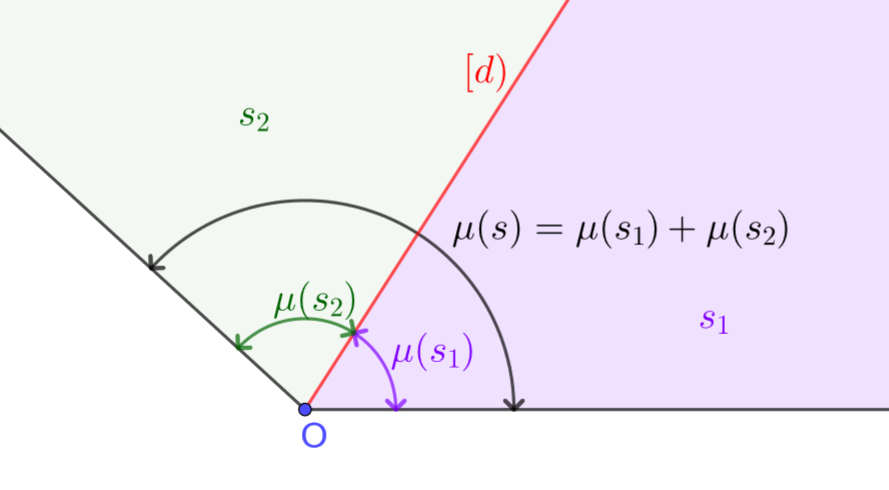
\includegraphics[width=0.7\textwidth]{image/thm_additivite_angles.png}
    \caption{Illustration de la propriété d'additivité des mesures d'angles lorsqu'on sépare un secteur d'angle par une demi-droite $[d)$ (en rouge sur la figure).}
    \label{fig_addi_angles}
\end{figure}
\begin{prop}
    Si deux secteurs d'angles on même mesure alors ils sont congruents.
\begin{scheme}
    On ramène le premier angle dans un des demi-plan du second avec l'isometrie canonique et on raisonne par l'absurde\,: si la demi-droite n'est pas envoyée sur l'autre alors on montre à l'aide de la proposition précédente que les mesures sont différentes. Donc forcément les demi-droites correspondent. La congruence se déduit de la définition de l'application canonique.
\end{scheme}
\end{prop}
\begin{thm}
    Deux secteurs d'angles on même mesure \ssi ils sont congruents. 
\end{thm}

    
    \section{Angles et orientation}

Au collège ou au lycée, la confusion entre angle et secteur d'angle est entretenue par les programmes officiels\,: le même mot \guil{angle} peut désigner un secteur d'angle (un lieu géométrique) ou une mesure d'angle (un nombre). L'égalité entre deux \guil{angles} sous-entendue par les élèves est celle de la mesure d'angle tandis que l'égalité des professeurs (non ignorants) et celles de la classe d'équivalence des secteurs d'angles sous relation d'isométrie. Autrement dit l'élève égalise deux \guil{angles} s'ils ont même mesure alors que le professeurs n'égalise ces \guil{angles} que s'il peut identifier une congruence entre le premier et le second.

\replaced[id=LB]{Dans les parties qui précèdent, nous avons établi}{Nous avons dans les partie qui précèdent établit} un grand nombre de résultats \replaced[id=LB]{sur}{concernant} les congruences entre secteurs d'angles. Il est pratique d'introduire alors les classes d'équivalence des secteurs d'angles sous la relation de congruence\,: l'angle.

        \subsection{Angles}

\begin{defi}[Angles]\label{defi-angle}
    Pour tout secteur d'angle saillant $s$ on appelle angle $\widehat{s}$ la classe d'équivalence de $s$ sous la relation de congruence, autrement dit,
    \begin{equation*}
        \widehat{s} = \ensemble{s' \text{ secteurs d'angles}}{s' \equiv \, s}\,.
    \end{equation*}
    
    Un angle $\mathcal{A}$ est alors un ensemble de secteurs d'angle tel qu'il existe un secteur d'angle $s$ tel que $\mathcal{A}=\widehat{s}$. 
\end{defi}

\begin{thm}[Identité de l'angle et de sa mesure]
Pour tout angle $\mathcal{A}$ il existe un unique $\mu_0\in ]0,\pi[$ tel que  pour tout $s \in \mathcal{A}$ on ait $\mu(s)=\mu_0$. $\mu_0$ est alors appelé mesure de l'angle $\mathcal{A}$. On note alors,
\begin{equation*}
    \mu\left(\mathcal{A}\right) = \mu_0\,. 
\end{equation*}
Inversement, pour tout nombre $\mu_0 \in ]0,\pi[$, il existe un unique angle $\mathcal{A}$ tel que $\mu\left(\mathcal{A}\right)=\mu_0$.
\end{thm}
\begin{rema}
    Ce théorème permet d'établir une relation univoque entre les angles et leurs mesures. Ceci justifie qu'on puisse parler indifféremment d'angle et de mesure d'angle. Désormais, donc, on identifie les mesures d'angles avec leurs angles\,: alors pour tout angle $\mathcal{A}$ on note (pas si) abusivement (que ça),
    \begin{equation*}
        \mathcal{A} = \mu \left(\mathcal{A}\right)\,.
    \end{equation*}
\end{rema}

        \subsection{Rotation du plan}

\begin{defi}[Orientations respectives des demi-plans orientés de même centre]
On dira que les demi-plans orientés $\overrightarrow{\mathcal{P}}_1 = \left(\mathcal{P}_1,]d_1)\right)$ et $\overrightarrow{\mathcal{P}}_2 = \left(\mathcal{P}_2,]d_2)\right)$ de même centre $O$ sont orientés en même façon \ssi
\begin{equation*}
    \mathcal{P}_1 \cap \mathcal{P}_2 %= s \quad \text{ou}\quad \mathcal{P}_1 \cap \mathcal{P}_2 = \bar{s}\,,
\end{equation*}
est un secteur d'angle saillant complémentaire de $\anglesaillant \left(O,]d_1),]d_2)\right)$. Sinon on dira qu'ils sont orientés différemment.
%où $s = \anglesaillant \left(O,]d_1),]d_2)\right)$ et $\bar{s}$ son secteur d'angle opposée par le sommet. 
\end{defi}
\begin{rema}
    Si $\overrightarrow{\mathcal{P}}_1 = \left(\mathcal{P}_1,]d_1)\right)$ et $\overrightarrow{\mathcal{P}}_2 = \left(\mathcal{P}_2,]d_2)\right)$ sont orientés différemment alors,
\begin{equation*}
    \mathcal{P}_1 \cap \mathcal{P}_2 = s \quad \text{ou}\quad \mathcal{P}_1 \cap \mathcal{P}_2 = \bar{s}\,,
\end{equation*}
où $s = \anglesaillant \left(O,]d_1),]d_2)\right)$ et $\bar{s}$ son secteur d'angle opposé par le sommet. 
\end{rema}
\begin{rema}
    La proposition \ref{prop-existetuniqueopposesommet} assure l'existence et l'unicité de $\bar{s}$
\end{rema}

\begin{prop}[Deux paires de plans orientés en même façon]\label{prop-pairsplanoriente}
    Soient $]d_1)$ et $]d_2)$ deux demi-droites de même extrémité $O$. 
    
    Notons $\mathcal{P}_1$ le demi-plan de droite support $(d_1)$ contenant $]d_2)$ et $\bar{\mathcal{P}_1}$ l'autre, $\mathcal{P}_2$ le demi-plan de droite support $(d_2)$ ne contenant pas $]d_1)$ et $\bar{\mathcal{P}_2}$ l'autre.

    Notons $\overrightarrow{\mathcal{P}}_1^+ = (\mathcal{P}_1,]d_1))$, $\overrightarrow{\mathcal{P}}_2^+ = (\mathcal{P}_2,]d_2))$, $\overrightarrow{\mathcal{P}}_1^- = (\bar{\mathcal{P}}_1,]d_1))$ et $\overrightarrow{\mathcal{P}}_2^- = (\bar{\mathcal{P}}_2,]d_2))$ les quatre plan orientés de centre $O$ qu'on peut construire avec les demi-droites $]d_1)$ et $]d_2)$. 

    Alors,
    \begin{itemize}[$\bullet$]
        \item $\overrightarrow{\mathcal{P}}_1^+$ et $\overrightarrow{\mathcal{P}}_2^+$ sont orientés en même façon,
        \item $\overrightarrow{\mathcal{P}}_1^-$ et $\overrightarrow{\mathcal{P}}_2^-$ sont orientés en même façon,
        \item tandis que $\overrightarrow{\mathcal{P}}_1^+$ et $\overrightarrow{\mathcal{P}}_2^-$ sont orientés différemment,
        \item $\overrightarrow{\mathcal{P}}_1^-$ et $\overrightarrow{\mathcal{P}}_2^+$ sont orientés différemment.
    \end{itemize}
\end{prop}

\begin{defi}[Rotation]
    Soient $]d_1)$ et $]d_2)$ deux demi-droite d'extrémité $O$. On reprend alors les notations de la proposition \ref{prop-pairsplanoriente}. On note également $]\bar{d_1})$ (respectivement $]\bar{d_2})$) la demi-droite ouverte supplémentaire de $]d_1)$ (respectivement $]d_2)$). 

    La rotation $R_{]d_1),]d_2)}$ envoyant $]d_1)$ sur $]d_2)$ est une application $R_{]d_1),]d_2)} : \mathcal{E} \to \mathcal{E}$ définie comme suit :
    \begin{equation*}
        \begin{array}{ccccc}
        R_{]d_1),]d_2)} & : &  \mathcal{E} & \to &  \mathcal{E} \\
         & & O & \mapsto & O \\
         & & M\in ]d_1) & \mapsto & M' \text{ le report de } [OM] \text{ sur } ]d_2) \\
         & & M\in ]\bar{d_1}) & \mapsto & M' \text{ le report de } [OM] \text{ sur } ]\bar{d_2}) \\
        & & M\in \mathcal{P}_1^+ & \mapsto & \mathcal{I}_{\overrightarrow{\mathcal{P}}_1^+,\overrightarrow{\mathcal{P}}_2^+} (M) \\
        & & M\in  \mathcal{P}_1^- & \mapsto & \mathcal{I}_{\overrightarrow{\mathcal{P}}_1^-,\overrightarrow{\mathcal{P}}_2^-} (M) \\
        \end{array}\,.
    \end{equation*}
\end{defi}
\begin{thm}
    Soient $]d_1)$ et $]d_2)$ deux demi-droites d'extrémité $O$\,; alors la rotation $R_{]d_1),]d_2)}$ envoyant $]d_1)$ sur $]d_2)$ est une isométrie. 
\end{thm}

        \subsection{Translation}

\begin{defi}[Translation]
    Soit $A$ et $B$ deux points, on appelle translation amenant $A$ sur $B$ l'application du plan $\tau_{\vb{AB}} : \mathcal{E} \to \mathcal{E}$ qui :
    \begin{itemize}[$\bullet$]
        \item à tout point $M$ en dehors de $(AB)$ associe l'unique point $M'$ intersection de l'unique parallèle à $(AB)$ passant par $M$ et de l'unique parallèle à $(AM)$ passant par $B$. 
        \item à tout point de $]AB)$ associe l'unique point $M'$ tel que $A\star M \star M'$ et $[AB]\equiv [MM']$
        \item à tout point de $(AB)-[AD)$ associe l'unique point $M'$ tel que $M\star M' \star B$ et $[AB]\equiv [MM']$
        \item à $A$ associe $B$.
    \end{itemize}
\end{defi}  
\begin{rema}
    L'axiome des parallèles \ref{axi-parra} assure l'univocité de cette application.
\end{rema}
\begin{thm}
    Soient $A$ et $B$ deux points alors $\tau_{\vb{AB}}$ la translation envoyant $A$ sur $B$ est une isométrie. 
\end{thm}

        \subsection{Inégalité triangulaire et conséquences}

Afin d'établir quelques propriétés \deletb{essentielles} des isométries qui nous serviront dans notre construction de la notion d'angle orienté, nous avons besoin d'un résultat essentiel\,: l'inégalité triangulaire. Celle-ci repose sur un série de lemmes\,:

%\begin{prop}\label{prop-rajlong}
%    Soit $A,B$ et $C$ trois points alors $AB \leq AB + BC$.
%\end{prop}

\begin{thm}[Théorème de l'angle extérieur]
    Soient $A,B$ et $C$ trois points distincts, alors dans le triangle $ABC$ la mesure de l'angle supplémentaire en $A$ est supérieur à l'angle en $A$ où en $B$.
% 4.12 dans le document pour les profs :https://publimath.univ-irem.fr/numerisation/LY/ILY98002/ILY98002.pdf
\end{thm}

\begin{lem}
Dans un triangle, si deux côtés n'ont pas même mesure alors les angles des sommets opposés aux côtés correspondants sont également de mesures différentes. De plus au côté le plus long est opposé le secteur d'angle de plus grande mesure. 
\end{lem}
\begin{lem}\label{lem-i3}
Dans un triangle, si deux angles aux sommets sont de mesures différentes alors les côtés opposés aux angles sommets correspondants sont également de mesures différentes. De plus à l'angle au sommet de plus grande mesure est opposé le côté de plus grande mesure.  
\end{lem}


\begin{thm}
Soient $A,B$ et $C$ trois points, alors,
\begin{equation*}
AB \leq AC + CD
\end{equation*}
où l'égalité est réalisé uniquement si $C\in [AB]$,
\begin{equation*}
    AB = AC + AD \quad \Longleftrightarrow \quad C\in [AB] 
\end{equation*}

\begin{proof}
On commence avec le cas de trois points $A,B$ et $C$ non-alignés (distincts et tel que $C\notin (AB)$). 

Notons $[d)$ la demi-droite fermée supplémentaire de la demi-droite ouverte $]CB)$ et notons (Axiome \ref{axi-C1}) l'unique point $D \in [d)$ tel que $CA\equiv CD$.  

Par construction on a $B\star C \star D$. En effet, les trois points appartenant à la même droite $(BC)$ respectent un alignement à trois points parmi trois possible (Axiome \ref{ax-B3}). Les deux autres possibles sont exclus du fait que $D \notin ]CB)$. 

Ainsi, $C \in ]DC[$ et donc (Prop. \ref{prop-barrtrans}) $C\in \anglesaillant \left( A,]AB),])AD)\right)$. Puis, en vertu de la proposition \ref{thm-incluspart}, on a,
\begin{equation*}
\anglesaillant \left( A,]AC),])AD)\right)\varsubsetneq \anglesaillant \left( A,]AB),])AD)\right)
\end{equation*}
et par suite,
\begin{equation*}
\anglesaillant \left( A,]AC),])AD)\right) < \anglesaillant \left( A,]AB),])AD)\right)\,.
\end{equation*}  

Or par construction $ACD$ est isocèle en $C$ et $]DC)=]DB)$ (car $C\in]BC[$) donc (Prop. \ref{prop-isocelecongruenceangle}),
 \begin{align*}
\anglesaillant \left( D,]DA),])DB)\right) \equiv \anglesaillant \left( D,]DA),])DC)\right)  \equiv \anglesaillant \left( A,]AC),])AD)\right) 
\end{align*}
et par compatibilité de la congruence avec la relation d'ordre sur le secteurs d'angle,
\begin{equation*}
    \anglesaillant \left( D,]DA),])DB)\right) < \anglesaillant \left( A,]AB),])AD)\right)\,.
\end{equation*}

En utilisant le Lemme \ref{lem-i3} dans le triangle $ABD$ (qui est non aplati car sinon cela voudrait dire que $A\in (BD)=(BC)$, et on a pris $A,B$ et $C$ non alignés) et sur les angles au sommets $A$ et $D$ que,
\begin{equation*}
AB<BD
\end{equation*}
or puisque $C\in ]BD[$ on peut utiliser la proposition \ref{prop-addlong} pour déduire que $BD=BC+CD$, enfin puisque $CD=AC$ on a,
\begin{equation*}
AB < AC + CB\,.
\end{equation*}

Dans le cas ou les points $A,B$ ou $C$ sont alignés il y a trois cas à considérer : 
\begin{itemize}[$\bullet$]
\item soit $A\star C \star B$ on  a $C \in ]AB[$ et donc (Prop. \ref{prop-addlong}) $AB = AC + CB$,
\item soit $C\star A \star B$ alors $A\in ]CB[$ et donc (définitions \ref{def-ineqlong}) $AB < BC$.  Ce qui implique $AB < BC \leq AC + CB $  (Prop. \ref{prop-addlong}). Ainsi, $ AB < AC + CB$.
\item soit  $A\star B \star C$, alors $B\in ]CA[$ et donc (définitions \ref{def-ineqlong}) $AB < AC$. De même (Prop. \ref{prop-addlong}) $AB < AC \leq AC + CB$. 
\end{itemize}
\end{proof}
\end{thm}

\begin{cor}
    L'image d'une droite (demi-droite, segment) par une isométrie est une droite (demi-droite, segment). 
\end{cor}

        \subsection{Secteur d'angle orienté}

\begin{defi}[Secteurs d'angles orienté]
    On appelle secteurs d'angle orientés les couples de demi-droite $o = \left(]d_1),]d_2)\right)$ de même extrémité. L'extrémité commune des demi-droite est appelé sommet de $o$.
\end{defi}
\begin{rema}
    Pour tout secteur d'angle orienté $o = \left(]d_1),]d_2)\right)$ de sommet $O$, on notera $\anglesaillant o = \anglesaillant \left(]d_1),]d_2)\right)= \anglesaillant\left(O,]d_1),]d_2)\right)$.
\end{rema}
\begin{defi}[Plan orienté associé à un angle orienté]
    Pour tout secteur d'angle orienté $\left(]d_1),]d_2)\right)$ on appelle demi-plan orienté associé le plan orienté $\overrightarrow{\mathcal{P}}=\left(\mathcal{P}_{(d_1),]d_2)},]d_1)\right)$.
\end{defi}
\begin{defi}[Orientation respective des secteurs d'angle orientés]
    Deux secteurs d'angle orientés sont orientés en même façon \ssi leurs demi-plans orientés associés le sont. \replaced[id=LB]{Sinon, on}{On} dit qu'ils sont orientés différemment\deletb{ sinon}. 
\end{defi}
\begin{prop}
    La relation d'orientation respective entre secteurs d'angle orientés est une relation d'équivalence.
\end{prop}
\begin{defi}[Plan orienté]
L'espace euclidien $\mathcal{E}$ est dit orienté \ssi il est muni d'un secteur d'angle orienté $r = \left(]d_I),]d_J)\right)$. On note $(\mathcal{E},r)$ l'espace euclidien orienté défini.
\end{defi}
\begin{defi}[Orientation]
Dans un plan euclidien orienté $(\mathcal{E},r)$ on dit que le secteur d'angle orienté $\left(]d_1),]d_2)\right)$ est orienté positivement \ssi $r$ et $\left(]d_1),]d_2)\right)$ sont orienté en même façon. Sinon on dira que l'angle orienté $\left(]d_1),]d_2)\right)$ est orienté négativement.
\end{defi}

        \subsection{Angle orienté}

\begin{defi}[Congruence entre angle orienté]
Soient $o_1$ et $o_2$ deux secteurs d'angle orientés\,; on dira que ces secteurs d'angles sont congruents \ssi $o_1$ et $o_2$ sont orientés en même façon et que $\anglesaillant o_1$ et $\anglesaillant o_2$ sont congruents. 

On notera également $\equiv$ cette relation.
\end{defi}
\begin{prop}
    La relation de congruence entre secteurs d'angle orientés est une relation d'équivalence.
\end{prop}
\begin{defi}[Angle orienté]
    Pour tout secteur d'angle orienté $o$ on appelle angle orienté $\widehat{o}$ de représentant $o$ la classe d'équivalence de $o$ sous la relation de congruence entre angles orientés, autrement dit,
    \begin{equation*}
        \widehat{o} = \ensemble{o' \text{ secteurs d'angles orient\'es}}{o' \equiv \, o}\,.
    \end{equation*}
    
    Un angle orienté $\mathcal{O}$ est alors un ensemble de secteurs d'angle orientés tel qu'il existe un secteur d'angle orienté $o$ tel que $\mathcal{O}=\widehat{o}$. 
\end{defi}

        \subsection{Mesure des secteurs d'angles orientés}

\begin{defi}[Mesure d'un angle orienté]
    Dans un plan euclidien orienté $(\mathcal{E},r)$ la mesure du secteur d'angle orienté $o$ est,
    \begin{equation*}
        \mu(o) = \pm \mu\left(\anglesaillant o\right)
    \end{equation*}*
    où $\pm = +$ si $r$ et $o$ sont orientés en même façon et $\pm = -$ sinon.
\end{defi}
\begin{thm}
    Soit $\mathcal{O}$ un angle orienté, alors il existe $\mu_0\in ]-\pi,\pi[$ tel que pour tout $o\in \mathcal{O}$ on a $\mu(o)=\mu_0$. On appellera alors mesure de $\mathcal{O}$ le nombre $\mu_0$. On note alors $\mu\left(\mathcal{O}\right)$ la mesure de l'angle orienté $\mathcal{O}$.  
\end{thm}
% reciproque
